%% abtex2-modelo-trabalho-academico.tex, v-1.9.2 laurocesar
%% Copyright 2012-2014 by abnTeX2 group at http://abntex2.googlecode.com/ 
%%
%% This work may be distributed and/or modified under the
%% conditions of the LaTeX Project Public License, either version 1.3
%% of this license or (at your option) any later version.
%% The latest version of this license is in
%%   http://www.latex-project.org/lppl.txt
%% and version 1.3 or later is part of all distributions of LaTeX
%% version 2005/12/01 or later.
%%
%% This work has the LPPL maintenance status `maintained'.
%% 
%% The Current Maintainer of this work is the abnTeX2 team, led
%% by Lauro César Araujo. Further information are available on 
%% http://abntex2.googlecode.com/
%%
%% This work consists of the files abntex2-modelo-trabalho-academico.tex,
%% abntex2-modelo-include-comandos and abntex2-modelo-references.bib
%%

% ------------------------------------------------------------------------
% ------------------------------------------------------------------------
% abnTeX2: Modelo de Trabalho Academico (tese de doutorado, dissertacao de
% mestrado e trabalhos monograficos em geral) em conformidade com 
% ABNT NBR 14724:2011: Informacao e documentacao - Trabalhos academicos -
% Apresentacao
% ------------------------------------------------------------------------
% ------------------------------------------------------------------------

\documentclass[
	% -- opções da classe memoir --
	12pt,               % tamanho da fonte
	openright,          % capítulos começam em pág ímpar (insere página vazia caso preciso)
	oneside,            % para impressão em verso e anverso. Oposto a oneside
	a4paper,            % tamanho do papel. 
	% -- opções da classe abntex2 --
	%chapter=TITLE,     % títulos de capítulos convertidos em letras maiúsculas
	%section=TITLE,     % títulos de seções convertidos em letras maiúsculas
	%subsection=TITLE,  % títulos de subseções convertidos em letras maiúsculas
	%subsubsection=TITLE,% títulos de subsubseções convertidos em letras maiúsculas
	% -- opções do pacote babel --
	english,            % idioma adicional para hifenização
	% french,             % idioma adicional para hifenização
	% spanish,            % idioma adicional para hifenização
	brazil              % o último idioma é o principal do documento
	]{abntex2}

% ---
% Pacotes básicos 
% ---
\usepackage{lmodern}            % Usa a fonte Latin Modern          
\usepackage[T1]{fontenc}        % Selecao de codigos de fonte.
\usepackage[utf8]{inputenc}     % Codificacao do documento (conversão automática dos acentos)
\usepackage{textcomp}
\usepackage{lastpage}           % Usado pela Ficha catalográfica
\usepackage{indentfirst}        % Indenta o primeiro parágrafo de cada seção.
\usepackage{color}              % Controle das cores
\usepackage[usenames,dvipsnames]{xcolor}
\usepackage{graphicx}           % Inclusão de gráficos
\usepackage{microtype}          % para melhorias de justificação
% ---
		
% ---
% Pacotes adicionais, usados apenas no âmbito do Modelo Canônico do abnteX2
% ---
\usepackage{lipsum}             % para geração de dummy text
% ---

% ---
% Pacotes de citações
% ---
\usepackage[brazilian,hyperpageref]{backref}     % Paginas com as citações na bibl
\usepackage[alf]{abntex2cite}   % Citações padrão ABNT
\usepackage{longtable}
\usepackage{soulutf8}				% Destaque de textos (highlight) com o comando \hl
\usepackage{framed}					% Borda em um paragrafo com \framed
\usepackage{listings}				% Para escrita de código
\usepackage{courier}				% Fonte Courier para os códigos
\usepackage{datetime}				% Datas customizadas
\usepackage{multirow}				% Multirow em tabelas
\usepackage{nameref}				% Mostra nome de ref

% Configurações para o Listing exibir os códigos na fonte Courier
\lstset{basicstyle=\footnotesize\ttfamily,breaklines=true}
%\lstset{framextopmargin=20pt,frame=bottomline}

% Para a citação de um anexo sair correta
\newcommand{\refanexo}[1]{\hyperref[#1]{Anexo~\ref{#1}}}

% --- 
% CONFIGURAÇÕES DE PACOTES
% --- 

% Cores

\definecolor{shadecolor}{HTML}{FFFFCC}
\definecolor{framecolor}{HTML}{FF0000}

% ---
% Configurações do pacote backref
% Usado sem a opção hyperpageref de backref
\renewcommand{\backrefpagesname}{Citado na(s) página(s):~}
% Texto padrão antes do número das páginas
\renewcommand{\backref}{}
% Define os textos da citação
\renewcommand*{\backrefalt}[4]{
	\ifcase #1 %
		Nenhuma citação no texto.%
	\or
		Citado na página #2.%
	\else
		Citado #1 vezes nas páginas #2.%
	\fi}%
% ---

% Numeracao de linhas
\newcounter{magicrownumbers}
\newcommand\rownumber{\stepcounter{magicrownumbers}\arabic{magicrownumbers}}

% Criando um novo tipo de coluna centralizado e com largura fixa
\newcolumntype{C}[1]{>{\centering\let\newline\\\arraybackslash\hspace{0pt}}m{#1}}

% Comando para notas para os orientadores

\newenvironment{frshaded}{%
\def\FrameCommand{\fboxrule=\FrameRule\fboxsep=\FrameSep \fcolorbox{framecolor}{shadecolor}}%
\MakeFramed {\FrameRestore}}%
{\endMakeFramed}

\renewcommand{\comment}[1]{
	\begin{frshaded}
		\noindent
		\textbf{Comentário:} #1
	\end{frshaded}
}

\newenvironment{textnew}{\color{Plum}}{}
\newenvironment{textedited}{\color{red}}{}

% Configs
\gdef\gitbranch{0.6.1}
\gdef\thesisdate{Mai 2015}
\gdef\githash{f17c385}


% Git support
% \input{gitinfo.tex}	

% ---
% Informações de dados para CAPA e FOLHA DE ROSTO
% ---
\titulo{Análise Comparativa de Ferramentas de Extração de Metadados em Artigos Científicos}
\autor{José Alberto Grossi Júnior}
\local{Belo Horizonte/MG, Brasil}
\data{\thesisdate, v-\gitbranch}
\orientador{Marcello Peixoto Bax}
\coorientador{Renato Rocha Souza}
\instituicao{%
	Universidade Federal de Minas Gerais -- UFMG
	\par
	Escola de Ciência da Informação
	\par
	Programa de Pós-Graduação em Ciência da Informação}
\tipotrabalho{Dissertação (Mestrado)}
% O preambulo deve conter o tipo do trabalho, o objetivo, 
% o nome da instituição e a área de concentração 
\preambulo{Dissertação de Mestrado apresentada à coordenação do PPGCI/UFMG com o objetivo de obtenção de título de Mestre em Ciência da Informação.}
% ---


% ---
% Configurações de aparência do PDF final

% alterando o aspecto da cor azul
\definecolor{blue}{RGB}{41,5,195}

% informações do PDF
\makeatletter
\hypersetup{
	%pagebackref=true,
	pdftitle={\@title}, 
	pdfauthor={\@author},
	pdfsubject={\imprimirpreambulo},
	pdfcreator={LaTeX with abnTeX2},
	pdfkeywords={extracao}{metadados}{artigos cientificos}{tecnicas de extracao}{machine learning}, 
	colorlinks=true,            % false: boxed links; true: colored links
	linkcolor=blue,             % color of internal links
	citecolor=blue,             % color of links to bibliography
	filecolor=magenta,              % color of file links
	urlcolor=blue,
	bookmarksdepth=4
}
\makeatother
% --- 

% --- 
% Espaçamentos entre linhas e parágrafos 
% --- 

% O tamanho do parágrafo é dado por:
\setlength{\parindent}{1.3cm}

% Controle do espaçamento entre um parágrafo e outro:
\setlength{\parskip}{0.2cm}  % tente também \onelineskip

% ---
% compila o indice
% ---
\makeindex
% ---

% ----
% Início do documento
% ----
\begin{document}

% Retira espaço extra obsoleto entre as frases.
\frenchspacing 

% ----------------------------------------------------------
% ELEMENTOS PRÉ-TEXTUAIS
% ----------------------------------------------------------
% \pretextual

% ---
% Capa
% ---
\imprimircapa
% ---

% ---
% Folha de rosto
% (o * indica que haverá a ficha bibliográfica)
% ---
\imprimirfolhaderosto*
% ---

% ---
% Inserir a ficha bibliografica
% ---

% Isto é um exemplo de Ficha Catalográfica, ou ``Dados internacionais de
% catalogação-na-publicação''. Você pode utilizar este modelo como referência. 
% Porém, provavelmente a biblioteca da sua universidade lhe fornecerá um PDF
% com a ficha catalográfica definitiva após a defesa do trabalho. Quando estiver
% com o documento, salve-o como PDF no diretório do seu projeto e substitua todo
% o conteúdo de implementação deste arquivo pelo comando abaixo:
%
% \begin{fichacatalografica}
%     \includepdf{fig_ficha_catalografica.pdf}
% \end{fichacatalografica}
\begin{fichacatalografica}
	\vspace*{\fill}                 % Posição vertical
	\hrule                          % Linha horizontal
	\begin{center}                  % Minipage Centralizado
	\begin{minipage}[c]{12.5cm}     % Largura
	
	\imprimirautor
	
	\hspace{0.5cm} \imprimirtitulo  / \imprimirautor. --
	\imprimirlocal, \imprimirdata-
	
	\hspace{0.5cm} \pageref{LastPage} p. : il. (algumas color.) ; 30 cm.\\
	
	\hspace{0.5cm} 
	
	\imprimirorientadorRotulo~\imprimirorientador\\
	\imprimircoorientadorRotulo~\imprimircoorientador\\
	
	\hspace{0.5cm}
	\parbox[t]{\textwidth}{\imprimirtipotrabalho~--~\imprimirinstituicao,
	\imprimirdata.}\\
	
	\hspace{0.5cm}
		1. Extração de metadados
		2. Metadados.
		I. Artigos científicos.
		II. Extração de informação.
		III. Ciência da Informação.
		IV. \imprimirtitulo\\            
	
	\hspace{8.75cm} CDU 02:141:005.7\\
	
	\end{minipage}
	\end{center}
	\hrule
\end{fichacatalografica}
% ---

% % ---
% % Inserir errata
% % ---
% \begin{errata}
% Elemento opcional da \citeonline[4.2.1.2]{NBR14724:2011}. Exemplo:

% \vspace{\onelineskip}

% FERRIGNO, C. R. A. \textbf{Tratamento de neoplasias ósseas apendiculares com
% reimplantação de enxerto ósseo autólogo autoclavado associado ao plasma
% rico em plaquetas}: estudo crítico na cirurgia de preservação de membro em
% cães. 2011. 128 f. Tese (Livre-Docência) - Faculdade de Medicina Veterinária e
% Zootecnia, Universidade de São Paulo, São Paulo, 2011.

% \begin{table}[htb]
% \center
% \footnotesize
% \begin{tabular}{|p{1.4cm}|p{1cm}|p{3cm}|p{3cm}|}
%   \hline
%    \textbf{Folha} & \textbf{Linha}  & \textbf{Onde se lê}  & \textbf{Leia-se}  \\
% 	\hline
% 	1 & 10 & auto-conclavo & autoconclavo\\
%    \hline
% \end{tabular}
% \end{table}

% \end{errata}
% ---

% ---
% Inserir folha de aprovação
% ---

% Isto é um exemplo de Folha de aprovação, elemento obrigatório da NBR
% 14724/2011 (seção 4.2.1.3). Você pode utilizar este modelo até a aprovação
% do trabalho. Após isso, substitua todo o conteúdo deste arquivo por uma
% imagem da página assinada pela banca com o comando abaixo:
%
% \includepdf{folhadeaprovacao_final.pdf}
%
\begin{folhadeaprovacao}

  \begin{center}
	{\ABNTEXchapterfont\large\imprimirautor}

	\vspace*{\fill}\vspace*{\fill}
	\begin{center}
	  \ABNTEXchapterfont\bfseries\Large\imprimirtitulo
	\end{center}
	\vspace*{\fill}
	
	\hspace{.45\textwidth}
	\begin{minipage}{.5\textwidth}
		\imprimirpreambulo
	\end{minipage}%
	\vspace*{\fill}
   \end{center}
		
   Trabalho aprovado. \imprimirlocal, \today:

   \assinatura{\textbf{\imprimirorientador} \\ Orientador} 
   \assinatura{\textbf{\imprimircoorientador} \\ Coorientador} 
   \assinatura{\textbf{Beatriz Valadares Cendón} \\ Professora Convidada - ECI/UFMG}
   \assinatura{\textbf{Max Cirino de Mattos} \\ Professor Convidado - UNA}
   \assinatura{\textbf{Renata M. Abrantes Baracho Porto} \\ Professora Suplente - ECI/UFMG}
	  
   \begin{center}
	\vspace*{0.5cm}
	{\large\imprimirlocal}
	\par
	{\large\imprimirdata}
	\vspace*{1cm}
  \end{center}
  
\end{folhadeaprovacao}
% ---

% ---
% Dedicatória
% ---
% \begin{dedicatoria}
%    \vspace*{\fill}
%    \centering
%    \noindent
%    \textit{Este trabalho é dedicado a todas as pessoas que desejam,\\ 
%    de uma forma ou outra, superar seus objetivos pessoais.} \vspace*{\fill}
% \end{dedicatoria}
% ---

% ---
% Agradecimentos
% ---
%\begin{agradecimentos}
%
%Os agradecimentos principais são direcionados a meu orientador Prof. Marcello Peixoto Bax, que me concedeu a oportunidade de realizar este trabalho com muita liberdade e com extrema confiança em meu trabalho.
%
%Agradecimentos especiais são direcionados aos meus pais por acreditarem em meu potencial e sempre aceitarem nas escolhas feitas por mim, sempre me incentivando de um modo ou outro a procurar sempre novos conhecimentos e experiências.
%
%Agradeço também de modo geral a todas as pessoas da ECI, tanto pelas amizades feitas quanto também por me apoiarem, me ouvirem e me incentivarem a acreditar no meu trabalho e a fazer um estudo de qualidade.
%
%\end{agradecimentos}
% ---

% ---
% Epígrafe
% ---
% \begin{epigrafe}
% 	\vspace*{\fill}
% 	\begin{flushright}
% 		\textit{``Não vos amoldeis às estruturas deste mundo, \\
% 		mas transformai-vos pela renovação da mente, \\
% 		a fim de distinguir qual é a vontade de Deus: \\
% 		o que é bom, o que Lhe é agradável, o que é perfeito.\\
% 		(Bíblia Sagrada, Romanos 12, 2)}
% 	\end{flushright}
% \end{epigrafe}
% ---

% ---
% RESUMOS
% ---

%!TEX root = ../masters.tex

% resumo em português
\setlength{\absparsep}{18pt} % ajusta o espaçamento dos parágrafos do resumo
\begin{resumo}
 % Segundo a \citeonline[3.1-3.2]{NBR6028:2003}, o resumo deve ressaltar o
 % objetivo, o método, os resultados e as conclusões do documento. A ordem e a extensão
 % destes itens dependem do tipo de resumo (informativo ou indicativo) e do
 % tratamento que cada item recebe no documento original. O resumo deve ser
 % precedido da referência do documento, com exceção do resumo inserido no
 % próprio documento. (\ldots) As palavras-chave devem figurar logo abaixo do
 % resumo, antecedidas da expressão Palavras-chave:, separadas entre si por
 % ponto e finalizadas também por ponto.

 % \textbf{Palavras-chaves}: latex. abntex. editoração de texto.

São inúmeras as ferramentas para extração de metadados em artigos científicos, tendo cada uma sua particularidade, tecnologia e técnicas utilizadas. Porém, com a crescente produção científica e a grande variedade de editoras, eventos e congressos, um grande número de artigos permanece sem uma extração de metadados eficaz, o que dificulta a disseminação de conhecimento e principalmente a pesquisa eletrônica destes documentos.

Este trabalho realiza um teste com algumas ferramentas pré-selecionadas com um conjunto pré-determinado de artigos, que abrange diversas áreas do conhecimento, diversos eventos e formatos visuais diferentes. Estes testes são realizados em ambientes pré-configurados de acordo com a necessidade tecnológica de cada ferramenta, permitindo que todos os artigos tenham seus metadados extraídos por cada uma delas e seus resultados comparados individualmente. 

Desta forma, com base nos resultados apresentados, pode-se identificar o comportamento de cada uma das ferramentas perante à extração de metadados, suas falhas, onde são necessários ajustes e onde se obtém um maior sucesso na extração. Além disso, é apresentado também o Índice de Confiabilidade, onde cada ferramenta recebe uma nota com base nos resultados obtidos na extração de metadados pela seleção de artigos realizada.

\textbf{Palavras-chaves}: artigos científicos, extração de metadados, extração de dados em artigos.

\end{resumo}

% resumo em inglês
\begin{resumo}[Abstract]
\begin{otherlanguage*}{english}

Currently we can find numerous tools to extract metadata from scientific papers, each one with your particularity, technology and techniques. However, with the crescent scientific production and the numerous publishers, events and conferences, a large part of papers still remain without an effective metadata extraction, hindering the knowledge dissemination e mainly the electronic search for these documents.

The present work makes tests with pre selected tools with a set of scientific papers, covering different areas of knowledge, different events and layouts. These tests were made inside custom environments according the technologies each tool needs, allowing all papers to be tested and their metadata extracted, comparing results one by one.

Thereby, according the presented results, we can identify the behavior of each tool related to the metadata extraction, where it failed, where adjusts are needed and where it has success on the extraction. Moreover, we also present the Reliability Index, a grade received by each tool based on the metadata extraction results using the selected scientific papers.

\textbf{Palavras-chaves}: scientific papers, metadata extraction, data extraction in scientific papers.

% \vspace{\onelineskip}

% \noindent 
% \textbf{Key-words}: latex. abntex. text editoration.
\end{otherlanguage*}
\end{resumo}

% resumo em francês 
% \begin{resumo}[Résumé]
%  \begin{otherlanguage*}{french}
% 	Il s'agit d'un résumé en français.
 
%    \textbf{Mots-clés}: latex. abntex. publication de textes.
%  \end{otherlanguage*}
% \end{resumo}

% % resumo em espanhol
% \begin{resumo}[Resumen]
%  \begin{otherlanguage*}{spanish}
%    Este es el resumen en español.
  
%    \textbf{Palabras clave}: latex. abntex. publicación de textos.
%  \end{otherlanguage*}
% \end{resumo}
% ---

% ---
% inserir lista de ilustrações
% ---
\pdfbookmark[0]{\listfigurename}{lof}
\listoffigures*
\cleardoublepage
% ---

% ---
% inserir lista de tabelas
% ---
\pdfbookmark[0]{\listtablename}{lot}
\listoftables*
\cleardoublepage
% ---

% ---
% inserir lista de abreviaturas e siglas
% ---
%!TEX root = ../masters.tex

\begin{siglas}
  \item[PDF] Portable Document Format
  \item[IEEE] Institute of Electrical and Electronics Engineers
  \item[RSL] Revisão Sistemática de Literatura
  \item[ACM] 
  \item[CAPES] Coordenação de Aperfeiçoamento de Pessoal de Nível Superior
  \item[XML] eXtensible Markup Language
  \item[SVM] Support Vector Machines
  \item[HMM] Hidden Markov Models
  \item[CRF] Conditional Random Fields
  \item[URL] Uniform Resource Locators
  \item[HTML] HyperText Markup Language
  \item[DCMI] Dublin Core Metadata Initiative
  \item[SVM] Support Vector Machines
  \item[DOI] Digital Object Identifier
\end{siglas}
% ---

% ---
% inserir lista de símbolos
% ---
% \begin{simbolos}
  % \item[$ \Gamma $] Letra grega Gama
  % \item[$ \Lambda $] Lambda
  % \item[$ \zeta $] Letra grega minúscula zeta
  % \item[$ \in $] Pertence
% \end{simbolos}
% ---

% ---
% inserir o sumario
% ---
\pdfbookmark[0]{\contentsname}{toc}
\tableofcontents*
\cleardoublepage
% ---



% ----------------------------------------------------------
% ELEMENTOS TEXTUAIS
% ----------------------------------------------------------
\textual

% Introdução
%!TEX root = ../masters.tex

\chapter{Introdução}
\label{cha:introduction}


\begin{figure}
    \centering
    \caption{Processo de Extração de Metadados}
    \label{fig:introduction}
    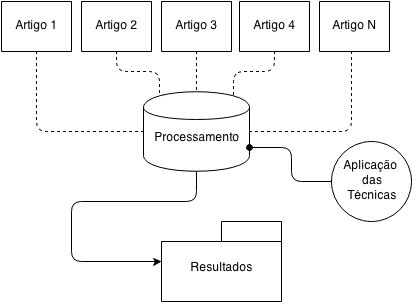
\includegraphics[width=0.9\linewidth]{./assets/images/introduction}
    \center\footnotesize{Fonte: O próprio autor}
\end{figure}

% \section{Contexto}
% \label{sec:context}

Em virtude da grande produção científica existente nos dias atuais, ferramentas automatizadas de extração de metadados em artigos científicos são cada vez mais úteis. Elas contribuem para uma melhor organização dos documentos e facilitam os processos de busca, tornando-os mais rápidos e eficientes.

A pesquisa aqui realizada situa-se no campo da extração de metadados segundo a abordagem \textit{machine learning}. O trabalho considera as ferramentas de código aberto mais populares atualmente. Diversas ferramentas e técnicas para extração de metadados em artigos podem ser encontradas na literatura científica da área de Ciência da Informação. 

Algumas ferramentas são propriedades de universidades ou instituições privadas, o que dificulta a análise. Outras não permitem que testes automatizados sejam feitos, visto que não há acesso ao código fonte ou não podem ser utilizadas via linha de comando.

De modo geral, as ferramentas de extração são focadas em leiautes pré-definidos, geralmente seguindo modelos (ou \textit{templates}) de revistas e encontros científicos, que possuem um padrão visual já estabelecido. Esse é o caso do IEEE (\textit{Institute of Electrical and Electronics Engineers}), por exemplo, que serve de referência para diversos outros eventos da área da Ciência da Computação. 

Porém, existem diversos outros eventos e revistas que empregam \textit{templates} específicos. A extração nesses artigos exige adaptações das ferramentas para que o processo seja satisfatório.

Algumas ferramentas são aparentemente muito eficazes para um certo grupo de artigos, já seguindo um padrão visual pré-determinado. Porém, para alguns \textit{templates} pouco comuns, de áreas de conhecimento diversas, elas não são tão eficazes. A eficácia varia de acordo com a tecnologia utilizada e, principalmente, de acordo com o princípio teórico utilizado.

Como definido por \cite{foundations-machine-learning}, \textit{machine learning} permite uma forma de aprendizado com base em experiências passadas, através da utilização de dados coletados, que são analisados posteriormente seguindo padrões definidos.

A área é muito ampla e sua aplicabilidade é diversificada, abrangendo necessidades específicas da Ciência da Informação, podendo ser usada na classificação, processamento de linguagem natural, reconhecimento de fala, detecção de fraudes, diagnósticos médicos e sistemas de recomendações, além de mecanismos de buscas e extração de informação. Essa última é a aplicação foco deste trabalho.

Claro que as técnicas de extração existentes hoje são, de maneira geral, insuficientes para tratar todos os leiautes de artigos existentes, limitando-se a apenas uma parcela destes, que usam padrões visuais comuns. Espera-se que certos artigos científicos não tenham seus metadados extraídos com total exatidão. Estes metadados são importantes para a produção científica, que exige  análises precisas para promover o acesso à informação.

Com base na diferenciação dos leiautes de artigos científicos, o objetivo da pesquisa é comparar o desempenho de ferramentas na tarefa de extração de metadados. Isso será feito com um conjunto de documentos pré-selecionados para testes, dos mais diversos padrões e de diversas áreas do conhecimento.

Espera-se com isso poder identificar o desempenho de tais ferramentas, suas limitações e melhores aplicações: quais ferramentas apresentam melhores resultados para cada padrão visual? Que ferramenta é melhor aplicada para determinado tipo distinto de metadado?

O documento é estruturado iniciando com essa breve introdução e motivação sobre o tema. O segundo capítulo traz o referencial teórico, onde são apresentados alguns conceitos básicos, além das técnicas mais utilizadas e as ferramentas mais comuns encontradas atualmente. O terceiro capítulo apresenta a metodologia usada no trabalho, citando as ferramentas que serão testadas e principalmente o método usado nesta pesquisa para a realização dos testes. Posteriormente, no capítulo quarto, faz-se a análise e apresentação dos resultados, explicando como os testes foram realizados, os ambientes de teste criados e os resultados coletados. No quinto capítulo temos a discussão final e a exposição de algumas conclusões mais relevantes, além dos trabalhos futuros e considerações finais sobre o trabalho apresentado.



% Referencial Teórico
%!TEX root = ../masters.tex

\chapter{Referencial Teórico}
\label{cha:literature}

A pesquisa é focada em técnicas e ferramentas para extração de metadados em artigos científicos. Cada ferramenta é testada juntamente com um grupo de artigos previamente selecionados. Estes artigos já possuem seus metadados extraídos manualmente, o que permite comparar os resultados com os resultados obtidos por cada uma das ferramentas. Os critérios utilizados serão de natureza explicitamente prática, numericamente representados.

Visando abranger grande parte da literatura sobre o assunto, alguns eventos e bases de dados importantes foram mapeados para a pesquisa, a fim de encontrar trabalhos relevantes para a área. Foram mapeados:

\begin{itemize}
    \item KDIR (International Conference of Knowledge Discovery and Information Retrieval);
    \item ICDAR (International Conference on Document Analysis and Recognition);
    \item PDCAT (International Conference on Parallel and Distributed Computing, Applications and Technologies);
    \item IAPR (International Workshop on Document Analysis Systems);
    \item ACM Conference on Digital Libraries.
\end{itemize}

Estes eventos foram analisados através da observação de todas as citações e referências utilizadas em cada artigo publicado, bem como outros detalhes importantes para a pesquisa.

\section{Metadados}
\label{sec:metadados}

\subsection{Conceito de Metadado}
\label{ssec:metadata-concept}

Com base nas ideias apresentadas por \cite{meta-dados}, ``[...] um elemento de metadado descreve um recurso de informação, ou ajuda a fornecer acesso a um recurso de informação.''. Todo dado que agregue nova informação a um recurso pode ser considerado um metadado. Quanto mais metadados um recurso tiver, mais detalhado ele é, ou seja, mais dados sobre ele se tem. Podemos simplificar ainda mais a definição de metadado como sendo ``um conjunto de dados sobre um determinado recurso''.

Podemos citar como exemplo a utilização de pequenos pedaços de dados sobre um conjunto de livros, dentro de um ambiente de biblioteca, o que é considerado uma coleção de elementos de metadados \cite{meta-dados}. O mesmo autor também cita como exemplos de metadados os dados coletados por mecanismos de busca no momento em que páginas da Internet são indexadas e então armazenadas.

\subsection{Padrões de Metadados}
\label{ssec:metadata-patterns}

Diante da infinidade de dados que podem estar atrelados a um determinado recurso, temos uma amplitude muito grande de características que podem ser definidas como sendo metadados. Por isso, foram definidos 15 (quinze) elementos para descreverem um recurso informacional, estabelecendo então um padrão adotado em todo o mundo, o padrão ``Dublin Core'' \cite{dublin-core}.

Este padrão se originou após uma série de encontros feitos desde 1995, unindo bibliotecários e pesquisadores digitais e de conteúdo, visando identificar padrões para se representar um recurso eletrônico. O nome ``Dublin'' foi dado em virtude da primeira reunião do grupo, que foi realizada na cidade de Dublin, Ohio. Já o nome ``Core'' se deu em virtude dos elementos serem amplos e genéricos, sendo então utilizados para descrever uma grande variedade de recursos.

Os quinze elementos que fazem parte do padrão Dublin Core compartilham de um vasto conjunto de vocabulários de metadados. Suas especificações técnicas são mantidas pela \emph{Dublin Core Metadata Initiative} (DCMI), agência responsável pela definição destes elementos.

Este padrão é utilizado nos dias atuais para se representar um recurso na Internet \cite{dublin-core-1-1}. Com base em suas características, mecanismos de buscas podem indexar um recurso de maneira mais rápida e precisa, pois este é acompanhado de pequenas sinalizações sobre seu conteúdo, apresentados em forma de metadados. 

Para cada elemento descrito pelo padrão temos informações como: 

\begin{itemize}
    \item \textit{label}, que é o texto para leitura e entendimento humano;
    \item \textit{name}, que é usado para o processamento de máquina, ou seja, um identificador único que a máquina utiliza para reconhecimento.
\end{itemize}

Os elementos que fazem parte da versão 1.1 do padrão Dublin Core \cite{dublin-core-1-1} podem ser vistos no \refanexo{attach:dublin-core} deste trabalho.

Abaixo podemos ver um exemplo de código para utilização de metadados Dublin Core em uma página da Internet, onde iremos referenciar os elementos \textit{creator}, \textit{title} e \textit{language}.

\lstset{language=HTML}
\begin{lstlisting}[escapechar=\#]
<meta name="DC.Creator" content="#\imprimirautor#" >
<meta name="DC.Title" content="#\imprimirtitulo#" >
<meta name="DC.Language" content="pt_BR" >
\end{lstlisting}

A indexação do autor (\textit{DC.Creator}) da página, bem como seu título (\textit{DC.Title}) e idioma (\textit{DC.Language}), são feitos de maneira bem simplificada e direta. Para páginas da Internet, com as informações todas em formato HTML, a utilização destes metadados perderia o sentido, visto que essas informações poderiam ser facilmente encontradas de outras formas, como a análise do próprio código. Para documentos binários - em formato PDF ou Word, por exemplo - a utilização destes metadados é de suma importância, visto que permite que essas informações básicas sejam capturadas sem a necessidade de análise do conteúdo destes arquivos.

\subsection{Técnicas de Extração de Metadados}
\label{ssec:metadata-techniques}

Algumas técnicas e algoritmos de extração de metadados são utilizadas em diversos projetos, variando de acordo com sua aplicação. Estas técnicas são baseadas na classificação de dados com base nas suas representações escritas, desde padrões preestabelecidos até com base em dicionários de palavras capazes de reconhecer ocorrências em diversas partes de um documento, o que garante assertividade ao processo de extração.

Técnicas de \emph{machine learning}, extração e classificação de dados utilizam, em sua grande maioria, dados de entrada previamente selecionados em forma semi-estruturada. Algumas bases de dados já consolidadas no mercado fornecem estes conjuntos de dados reais, compostos por artigos científicos catalogados internamente, que são utilizados como documentos de entrada para a análise e desenvolvimento de novas pesquisas.

Com a utilização destes \emph{datasets}\footnote{Conjuntos de dados estruturados semanticamente fornecidos por diversas entidades/órgãos para serem utilizados para fins de pesquisa.} o processo de teste fica muito mais fácil. Existem algumas técnicas que possuem melhor desempenho ao se utilizar dos chamados \emph{training sets}, que são por definição estes \emph{datasets} utilizados para treinar um determinado modelo, promovendo um padrão de extração com base em dados previamente informados.

\subsubsection{Regular Expressions (RegEx)}
\label{sssec:regular-expressions}

No caso específico de extração de metadados a utilização de \emph{Regular Expressions} (ou Expressões Regulares) é muito eficaz no reconhecimento de padrões, como é o caso do metadado e-mail, por exemplo, que possui um formato muito específico. É uma técnica muito utilizada na computação para reconhecimento de padrões dentro de um conjunto de caracteres, encontrando combinações seguindo uma sequência definida.

Sua origem data-se de 1956 \cite{kleene-1956}, sendo fundamentada pelo matemático Stephen Kleene, que deu origem à Teoria da Computação. Somente em 1968 que as expressões regulares ficaram conhecidas, através de Ken Thompson \cite{thompson-1968}, que incluiu a pesquisa de Kleen como funcionalidade dentro de um editor de textos, permitindo então que padrões fossem encontrados dentro de arquivos.

Para a utilização de Expressões Regulares é necessário o fornecimento de um padrão, que será a base de busca em todo o conjunto de caracteres existente. Este padrão é representado por um conjunto de símbolos, que determina a forma desejada de reconhecimento. Assim, além de utilizar-se de caracteres específicos pode-se também informar números, letras, dentre outros tipos de representação, correspondendo ao que se deseja reconhecer dentro do texto.

Existem variações de formas de representação de uma Expressão Regular, porém, a maioria das linguagens de programação atualmente seguem o padrão POSIX (\emph{Portable Operating System Interface}) - sob responsabilidade do IEEE e do Open Group \url{http://opengroup.org/} -, que determina algumas regras para utilização desta técnica \cite{posix-2013}.

Como exemplo, visando identificar somente os números existentes dentro da frase ``Foram encontrados 4 passageiros dentro do veículo parado na BR262.'', devemos escrever uma expressão regular para que estes números sejam identificados. Desta forma podemos representar o que desejamos buscar da seguinte forma: \texttt{/[0-9]+/}, onde identificamos:

\begin{itemize}

    \item o uso do caractere \texttt{/}, que determina o começo e fim da expressão regular;
    
    \item a representação de algarismos utilizando \texttt{[0-9]}, que significa qualquer dígitos de 0 a 9, permitindo que os números sejam identificados dentro do texto; 
    
    \item a existência de números com mais de um dígito, como é o caso de \texttt{262}, necessitando complementar o padrão para permitir um ou mais algarismos, o que é representado pelo caractere de repetição \texttt{+}, que significa exatamente ``uma ou mais ocorrências''.

\end{itemize}

Em diversas ocasiões é necessária a utilização de repetições, informando que aquele padrão pode ocorrer diversas vezes. Assim, temos as seguintes formas de representação para repetições:

\begin{itemize}

    \item Como pode ser observado no exemplo acima, utilizamos o caractere \texttt{+} para representar ``uma ou mais ocorrências''. No exemplo \texttt{[0-9]+} representamos qualquer número que possua um ou mais dígitos de 0 a 9.
    
    \item Já o caractere \texttt{?} (interrogação) pode ser utilizado para representar ``nenhuma ou apenas uma ocorrência'', ou seja, aquele padrão pode ou não existir, é opcional. Na expressão regular \texttt{[0-9]?} estamos informando que o dígito é opcional, ou seja, ele pode ou não estar presente no texto.
    
    \item Podemos utilizar o caractere \texttt{*} (asterisco) para representar ``nenhum ou mais'', ou seja, podemos ter nenhuma ou várias ocorrências daquele conjunto, indo do zero ao infinito.

\end{itemize}

Além das repetições, em alguns momentos necessitamos identificar um número exato de caracteres. Para identificar um ano de 4 (quatro) dígitos, necessitamos informar que o padrão deve ser identificado para apenas 4 dígitos, nem mais, nem menos. Desta forma temos as seguintes formas de representação:

\begin{itemize}

    \item Para número de ocorrências exatos utilizamos da expressão regular \texttt{[0-9]\{4\}}, que exige que para identificação do padrão o número tenha exatamente 4 dígitos de 0 a 9.

    \item Podemos estipular quantidade mínima de repetições, como por exemplo \texttt{[0-9]\{3,\}}, que significa ``qualquer número que possua no mínimo 3 dígitos'', ou seja, os números 123, 481145, 9182 seriam identificados, mas 14 não, visto que possui apenas 2 dígitos.

    \item Podemos também estipular apenas a quantidade máxima desejada, como \texttt{[0-9]\{,8\}}, ou seja, somente os números que possuem até no máximo 8 dígitos. Neste caso, um número com 9 ou mais dígitos não entraria no reconhecimento de padrão.

    \item Por fim, tomando como base os dois últimos exemplos, podemos informar os valores mínimo e máximo ao mesmo tempo, como \texttt{[0-9]\{4,8\}}, ou seja, números que possuem no mínimo 4 dígitos e no máximo 8 dígitos.

\end{itemize}

Desta forma podemos consolidar as formas de repetição em Expressões Regulares com base na \autoref{tab:regex-repeticao}.

\begin{table}
    \caption{Formas de representação de repetições em Expressões Regulares.}
    \begin{center}
        \begin{tabular}{|c|l|}
            \hline 
            \textbf{Forma de Representação} & \textbf{Significado} \\ 
            \hline 
            \texttt{?} & Nenhuma ou apenas uma ocorrência \\
            \hline 
            \texttt{*} & Nenhuma ou várias ocorrências \\
            \hline
            \texttt{+} & Uma ou mais ocorrências \\
            \hline
            \texttt{\{4\}} & Exatamente 4 ocorrências \\
            \hline
            \texttt{\{4,\}} & No mínimo 4 ocorrências \\
            \hline
            \texttt{\{,8\}} & No máximo 8 ocorrências \\
            \hline
            \texttt{\{4,8\}} & No mínimo 4 e no máximo 8 ocorrências \\
            \hline
        \end{tabular}
    \end{center}
    \label{tab:regex-repeticao}
\end{table}

Além dos dígitos podemos representar também caracteres puros, utilizando-se também do operador \texttt{|} (chamado \emph{pipe} em inglês), que representa alternância, usado quando temos mais de uma opção. Tomemos a frase ``O amor da vida de Ana se chama Paulo''. Para identificar o reconhecimento dos nomes próprios nesta frase podemos utilizar o padrão \texttt{/Ana|Paulo/}, que quer dizer ``Ana \underline{ou} Paulo''.

Utilizando-se do caractere de alternância \texttt{|} ainda podemos utilizá-lo em conjunto com outros caracteres. Na expressão regular \texttt{/abaca(te|xi)/}, podemos identificar as palavras ``abacate'' ou ``abacaxi'', preservando os caracteres \texttt{abaca} e alternando entre as opções \texttt{te} ou \texttt{xi}. Neste caso utilizamos parênteses para representar grupos de caracteres. Caso utilizássemos o padrão sem os parênteses - \texttt{abacate|xi} - iríamos ser capazes de identificar apenas as palavras ``abacate'' ou a palavra ``xi''.

A aplicação de expressão regular é bastante variada, existindo diversas formas de representação de qualquer padrão necessário. Além dos detalhes já explicados acima, existem os chamados ``metacaracteres'', que possuem significados definidos em uma expressão regular, assim como \texttt{+} e \texttt{?}, mas com outras formas de representação e objetivos.

\begin{itemize}

    \item O ponto (\texttt{.}) possui um significado muito importante, sendo considerado ``qualquer coisa''. Assim, a expressão regular \texttt{/abaca../} permite que \texttt{abacaxi} e \texttt{abacate} também sejam identificados. Ela representa ``qualquer coisa que comece com \texttt{abaca} e possui mais 2 caracteres quaisquer depois''. Ou seja, além de identificar \texttt{abacate} e \texttt{abacaxi} ela permite identificar \texttt{abaca17} ou até mesmo \texttt{abaca s}, visto que espaço também é um caracteres e faz parte do reconhecimento de \texttt{.}.

    \item Os colchetes - já vistos anteriormente - representam um conjunto de caracteres únicos dentro de várias possibilidades. Isso quer dizer que em \texttt{/[abc]/} desejamos identificar qualquer um dos caracteres \texttt{a}, \texttt{b} ou \texttt{c}. Assim, dentro da palavra \texttt{casa} conseguimos identificar a letra \texttt{c} e a letra \texttt{a}.

    \item O acento circunflexo (\texttt{\textasciicircum}) possui significado de negação quando presente dentro de colchetes. Com base no exemplo acima (\texttt{/[abc]/}), caso ele seja escrito como \texttt{/[\textasciicircum{abc}]/}, seu significado é exatamente o oposto, representando quaisquer caracteres exceto \texttt{a}, \texttt{b} e \texttt{c}. Além deste significado, ele é utilizado para representar o início de algum padrão no seu texto de origem. Na expressão regular \texttt{/\textasciicircum{a.+}/} temos o seguinte significado: ``um texto que comece com a letra \texttt{a} seguido de qualquer caractere em qualquer quantidade''. Desta forma, com esta expressão, conseguimos identificar \texttt{abcd}, \texttt{ab}, \texttt{abcdefghijk} e até mesmo \texttt{a9715263}. A única exigência, neste caso, é começar com a letra \texttt{a}, de maneira que no texto ``as mulheres marcaram presença'' seremos capaz de identificar toda a frase, mas já em ``todas as mulheres marcaram presença'' ela não identificará nada, visto que o texto começa com a letra \texttt{t}.

    \item Assim como o \texttt{\textasciicircum} representa o início de uma Expressão Regular o \texttt{\$} indica o fim. A lógica é a mesma, se aplicando para todo o texto, e não apenas em ocorrências isoladas. Assim, para a expressão \texttt{/\textasciicircum{a.+z}\$/} exige-se que o texto comece com a letra \texttt{a} e termine com a letra \texttt{z}.

    \item Já os parênteses - \texttt{(} e \texttt{)} - representam grupos. Estes grupos, além de serem utilizados como no exemplo \texttt{/abaca(te|xi)/}, podem ser utilizados para substituição de ocorrências, aumentando ainda mais a aplicação de expressões regulares. Como exemplo, dentro do texto ``os estudantes adoram comer abacaxi depois do almoço'', podemos substituir toda ocorrência de \texttt{abacaxi} por qualquer outra palavra, como \texttt{melão}. Para isso temos que formar um grupo com a palavra \texttt{abacaxi}, escrevendo a expressão regular da seguinte maneira: \texttt{/(abacaxi)/}. Assim, será reconhecida a palavra completa e esta poderá ser substituída por \texttt{melão}, ficando a frase ``os estudantes adoram comer melão depois do almoço''.

\end{itemize}

Em virtude da existência dos ``metacaracteres'' - os caracteres especiais que possuem significados específicos nas Expressões Regulares -, caso seja necessária a representação de algum em sua forma pura, utiliza-se do caractere de escape \texttt{\textbackslash{}} (barra invertida) antes do caractere desejado. Por exemplo, para escrever o símbolo \texttt{+}, literalmente, deve-se representá-lo por \texttt{\textbackslash{+}}. Desta forma a expressão será interpretada como um ``mais'' e não como um caractere de repetição.

Assim como vimos a utilização de \texttt{0-9} para representação de dígitos, temos outras representações, tanto para indicar letras maiúsculas quanto minúsculas, utilizando de \texttt{A-Z} e \texttt{a-z}, respectivamente. Sendo assim, podemos identificar dígitos, letras minúsculas e maiúsculas com a expressão regular \texttt{/[A-Za-z0-9]+/}. Além disso, no padrão POSIX podemos representar conjuntos de letras e números de outras formas chamadas ``classes'', como pode ser verificado na \autoref{tab:posix-classes}.

\begin{table}
    \caption{Classes do padrão POSIX.}
    \begin{center}
        \begin{tabular}{|l|p{6cm}|l|}
            \hline 
            \textbf{POSIX} & \textbf{Equivalência} & \textbf{Descrição} \\ 
            \hline 
            \texttt{[:alnum:]} & \texttt{[A-Za-z0-9]} & Caracteres alfanuméricos \\
            \hline
            \texttt{[:alpha:]} & \texttt{[A-Za-z]} & Caracteres alfabéticos \\
            \hline
            \texttt{[:blank:]} & \texttt{[ \textbackslash{t}]} & Espaço e tabulação (tab) \\
            \hline
            \texttt{[:cntrl:]} & \texttt{[\textbackslash{x}00-\textbackslash{x}1F\textbackslash{x}7F]} & Caracteres de controle ASCII \\
            \hline
            \texttt{[:digit:]} & \texttt{[0-9]} & Dígitos \\
            \hline
            \texttt{[:graph:]} & \texttt{[\textbackslash{x}21-\textbackslash{x}7E]} & Caracteres visíveis \\
            \hline
            \texttt{[:lower:]} & \texttt{[a-z]} & Letras minúsculas \\
            \hline
            \texttt{[:print:]} & \texttt{[\textbackslash{x}20-\textbackslash{x}7E]} & Caracteres visíveis e espaço \\
            \hline
            \texttt{[:punct:]} & \texttt{[][!"\#\$\%\&'()*+,./:;\textless=\textgreater?@\newline\textbackslash\textasciicircum\_`\{\textbar\}\textasciitilde-]} & Caracteres de pontuação \\
            \hline
        \end{tabular}
    \end{center}
    \label{tab:posix-classes}
\end{table}

% Falar de flags também -> não incluído por ser específico de linguagens de programação

As aplicações de Expressões Regulares são infinitas, sendo capazes de identificar qualquer sequência que possa ser representada em forma de texto, como telefones, endereços, dentre outras, o que facilita muito o reconhecimento de padrões, inclusive para a área de extração de dados.

% Escrever sobre

\subsubsection{Support Vector Machines (SVM)}
\label{sssec:svm}

\emph{Support Vector Machines} (SVM) é uma técnica de \textit{machine learning} que permite que um conjunto de dados seja analisado através do reconhecimento de padrões, formando uma memória \cite{Vapnik-SVM}. Seu objetivo inicial era ser uma técnica de classificação de dados, por ser focada em reconhecimento de padrões através de análises matemáticas.

Esta técnica é baseada na redução de erros com base em um resultado de treinos consecutivos que permitem a criação de um padrão e estabelecem um aprendizado com base na distância entre ocorrências \cite{Vapnik-SVM}. Todas as análises realizadas são mapeadas, permitindo que um registro histórico em forma matemática seja realizado, levando o algoritmo à possibilidade de diferenciação numérica entre um resultado e outro.

De acordo com Chieu \cite{Chieu}, sugere-se que a tarefa de extrair informação pode ser considerada um problema de classificação. Partindo deste pensamento foi que Han \cite{Han-SVM} decidiu utilizar técnicas de SVM para extração de metadados, utilizando das qualidades matemáticas do processo no reconhecimento de padrões, o que permitiu que novas descobertas fossem feitas, expandindo o estudo da extração de dados para um patamar mais amplo e elevado.

Várias ferramentas de extração se baseiam na utilização de SVM como técnica principal, visto sua eficiência no reconhecimento de padrões. Como descrito por \cite{Han-SVM} a utilização desta técnica é baseada na identificação de campos previamente selecionados no cabeçalho de um documento, por exemplo.

Esta técnica analisa diversos campos chamando-os de classes, e atribui a cada uma características que permitem que ela seja identificada. Deste modo, cada linha do cabeçalho do documento é classificada em uma ou mais classes. Algumas dessas classes fazem parte do padrão Dublin Core, conforme detalhado na \autoref{ssec:metadata-patterns}.

Seymore et al. \cite{Seymore-HMM-IE} definiram 15 (quinze) \textit{tags} para esta definição do cabeçalho de um documento. Porém, destas somente 4 (quatro) correspondem ao padrão da Dublin Core e estão ilustradas na \autoref{tab:svm-classes}. Estas também foram as \textit{tags} utilizadas por Han na extração de metadados dos cabeçalhos de artigos científicos \cite{Han-SVM}.


\begin{table}
    \caption{Relação de classes utilizadas e comparação com o padrão Dublin Core.}
    \begin{center}
        \begin{tabular}{|C{3cm}|C{3cm}|p{7cm}|}
            \hline \textbf{Classe (Tag)} & \textbf{Referência Dublin Core} & \textbf{Descrição}\\ 
            \hline Title & Title & Título do artigo\\
            \hline Author & Creator & Nome do autor do documento\\
            \hline Affiliation & & Afiliação do autor\\
            \hline Address & & Endereço do autor\\
            \hline Note & & Frases de reconhecimentos, \textit{copyright}\\
            \hline Email & & Endereço de e-mail do autor\\
            \hline Date & & Data da publicação\\
            \hline Abstract Introdution & Description & A introdução ou resumo do artigo\\
            \hline Phone & & Telefone do autor\\
            \hline Keyword & Subject & As palavras-chave do documento\\
            \hline Web & & Endereço na Web do autor\\
            \hline Degree & & Associação com o grau acadêmico\\
            \hline Pubnum & & Número da publicação do documento\\
            \hline Page & & O final da página\\
            \hline
        \end{tabular}
    \end{center}
    \label{tab:svm-classes}
\end{table}

A ocorrência dos campos é mapeada em uma representação bidimensional, o que permite identificar visualmente os padrões encontrados na análise de cada classe. Desta forma, com a visualização do posicionamento de cada ocorrência é possível obter uma distância clara entre os pontos de reconhecimento, chamada pelo autor de \textit{hyperplanes} \cite{Vapnik-SVM}. Por sua vez, estes pontos são marcados como sendo os ``support vectors'', e permitem que o \textit{hyperplane} entre eles determine a divisão entre as classes de forma clara e eficaz, como pode ser visto na \autoref{fig:svm-graph}. Esta divisão permite então a distinção entre os metadados, diferenciando os elementos analisados pelo algoritmo.

\begin{figure}
    \centering
    \caption{Distância representando a separação entre classes na técnica de SVM.}
    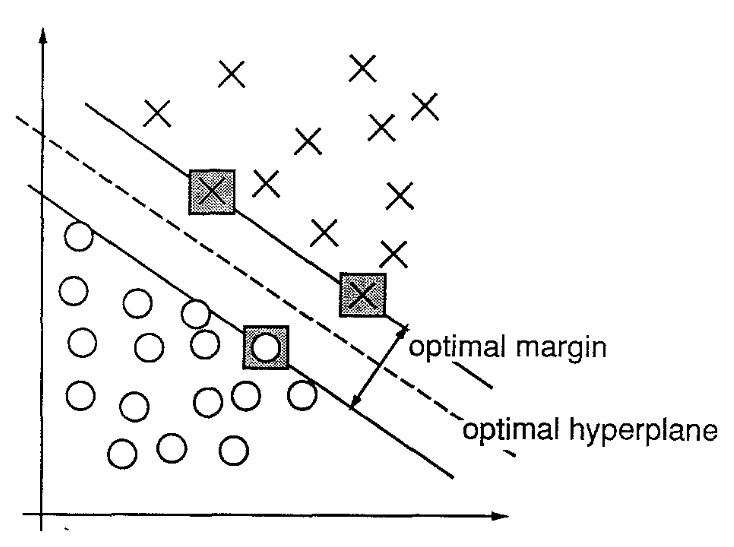
\includegraphics[width=0.6\linewidth]{./assets/images/svm-graph}
    \center\footnotesize{Fonte: \cite{Vapnik-SVM}}
    \label{fig:svm-graph}
\end{figure}

Além desta análise também são utilizadas comparações de palavras dentro de um contexto, através do uso de \textit{clusters} de palavras, que facilita a identificação de classes nos cabeçalhos analisados. Han \cite{Han-SVM} utiliza em suas análises \textit{clusters} com palavras comuns, compostos por:

\begin{itemize}
    \item Dicionário online padrão em sistemas Linux;
    \item 8.441 nomes e 19.613 sobrenomes;
    \item Sobrenomes chineses;
    \item Nomes dos estados dos Estados Unidos e das províncias canadenses;
    \item Nomes das cidades dos Estados Unidos;
    \item Nome dos países do mundo, de acordo com World Fact Book\footnote{Disponível em \url{https://www.cia.gov/library/publications/the-world-factbook/index.html}};
    \item Nome dos meses e suas respectivas abreviações.
\end{itemize}

Para cada uma das classes analisadas são feitas correlações com o tipo de dado esperado, que permite extrair, por exemplo, endereços de e-mail com base em expressões regulares utilizadas em linguagens de programação.

\emph{Support Vector Machines} é uma técnica conhecida principalmente por sua boa performance e habilidade para com grandes quantidades de dados, sendo por isso considerada uma boa solução para problemas de classificação. Por essa característica, sua principal funcionalidade é baseada na comparação entre um conjunto de opções, identificando as semelhanças e permitindo classificações. Por isso, Han \cite{Han-SVM} decidiu utilizar este mesmo conceito na extração de dados, confrontando e comparando classes de metadados, para posterior identificação e diferenciação.

Han também encontrou alguns desafios na diferenciação de campos, como é o caso dos múltiplos autores. Em alguns casos a diferenciação de autores, que fazem parte do mesmo campo, poderia estar em linhas ou grupos diferentes. Para isso foram utilizados alguns elementos para representar a separação dos nomes (\textit{chunks}), como pontuações e a presença da palavra ``and''. Desta forma, os autores eram extraídos seguindo este padrão estipulado.

O resultado obtido pela utilização de SVM como técnica de extração de metadados foi bem relevante. O autor realizou uma comparação com a aplicação da técnica de \emph{Hidden Markov Models} (HMM) - detalhada na \autoref{sssec:hmm} - onde a SVM se mostrou mais eficaz na extração para algumas classes específicas, como é o caso dos títulos, autores e endereços, por exemplo. Para outras classes a utilização da técnica de HMM ainda demonstrou ser mais eficiente na extração de metadados.

\subsubsection{Hidden Markov Models (HMM)}
\label{sssec:hmm}

A teoria básica de Markov foi conhecida próximo dos anos 80 por engenheiros e matemáticos, com grande aplicação inicialmente em processamento da fala, mas com vasta amplitude em outras áreas onde a descoberta de padrões pode ser aplicada \cite{Rabiner-HMM}.

O processo é baseado na identificação de modelos observáveis que representem e caracterizem a ocorrência de símbolos, ou seja, padrões. Se um sinal é observado ele pode ser utilizado para futuras referências, de acordo com o padrão estipulado. 

Um exemplo prático citado por Rabiner e Juang \cite{Rabiner-HMM} é o caso de uso do jogo ``Cara e Coroa''. Toma-se um observador em um quarto fechado com uma cortina, isolando totalmente qualquer outro cômodo. Este observador não consegue ver nada que acontece do outro lado, onde está presente uma outra pessoa jogando uma moeda pra cima, relatando sempre o resultado obtido (cara ou coroa). Neste caso o problema é construir um modelo Hidden Markov Model (HMM) para explicar ao observador a sequência dos resultados obtidos. 

Neste exemplo, o primeiro caso é baseado tanto no estado de cada resultado (cara ou coroa) e em probabilidades matemáticas de ocorrências destes estados, neste caso, 0.5 (50\%), ou seja, dois estados totalizando 100\%. Assim desenha-se modelos onde os estados são representados com base nas inúmeras possibilidades existentes, levando inclusive em consideração a sequência dos últimos acontecimentos. Outra possibilidade seria a existência de duas moedas, o que daria ainda dois estados existentes, mas não em função da probabilidade de sair cara ou coroa, mas sim por serem consideradas duas moedas ``justas'', o que daria também uma probabilidade de 0.5 para cada.

Neste último exemplo o grande detalhe do modelo é que este é oculto (\textit{hidden}). Isso se deve ao fato de os dois estados, representados pelas duas moedas, serem totalmente independentes, o que não permite identificar qual moeda é a ``justa'' e então informar ao observador o resultado daquela rodada.

Por esta alteração de resultados e probabilidades, o fator decisivo na criação de cada modelo é a definição do número de estados que ele terá. Além disso, outro ponto que determina o sucesso do método é a utilização de um resultado anterior - os \textit{training datasets} -, ou seja, uma memória, um conjunto de informações pré-identificadas que permite ainda à associação dos estados e ocorrência dos símbolos \cite{Rabiner-HMM}.

Um HMM pode ser formado por um conjunto de elementos, compondo toda a teoria e a aplicação dos algoritmos dentro do processo:

\begin{enumerate}
    \item Um número \texttt{N} de estados, onde \texttt{N} é um inteiro finito;
    \item Um intervalo temporal \texttt{t}, que determina a entrada em um novo estado, através de uma transição de probabilidade entre eles, levando em consideração sempre o estado anterior;
    \item Após cada transição o observador registra um \texttt{símbolo} de acordo com a distribuição de probabilidade, que por sua vez depende do estado atual do modelo.
\end{enumerate}

A utilização dos resultados passados - \textit{training datasets} - é muito importante para uma boa definição de um HMM, visto que permite adaptar os parâmetros do modelo para aquele conjunto de dados passados, que por sua vez fazem parte de um padrão já identificado e treinado.

Seguindo este padrão o HMM pode ser utilizado, por exemplo, para reconhecimento de palavras isoladas que, juntamente com a utilização de um vocabulário previamente selecionado, permite a criação de modelos de reconhecimento. Cada palavra deste vocabulário seria um modelo HMM, permitindo que a palavra escolhida fosse a pertencente ao modelo com maior probabilidade encontrada.

Já no âmbito da extração da informação, o HMM pode ser aplicado conforme é apresentado por Seymore et al. \cite{Seymore-HMM-IE}, onde um modelo construído manualmente contendo múltiplos estados por campos (título, autor, etc), pode ser mais eficiente do que um modelo com somente um estado por campo. 

\begin{figure}
    \centering
    \caption{Exemplo de modelo HMM, onde ``X'' são os estados, ``Y'' as observações possíveis, ``A'' as probabilidades de mudança de estado e ``B'' as saídas destas probabilidades.}
    \label{fig:hmm-states}
    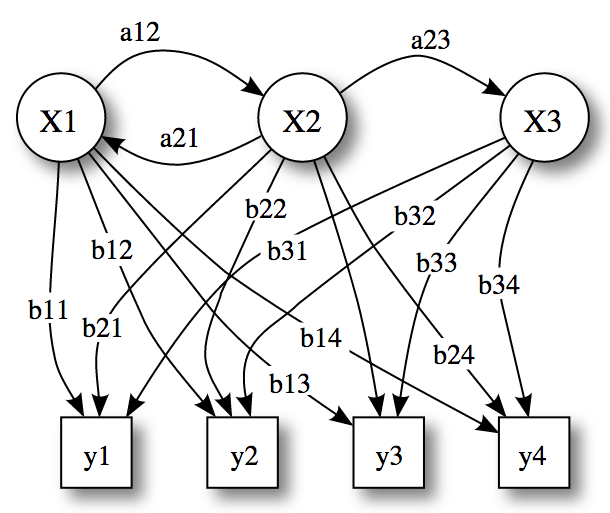
\includegraphics[width=0.7\linewidth]{./assets/images/hmm-states}
    \center\footnotesize{Fonte: Wikipedia / Hidden Markov Model \url{http://goo.gl/pI3XUU}}
\end{figure}

Um dos pontos positivos deste modelo é que por ser baseado em estatística ele é muito bem empregado em problemas de linguagem natural, aliando os resultados positivos à excelente performance computacional. Como desvantagem desta técnica podemos citar o fato de, por ser baseada em estatística matemática, uma grande quantidade prévia de dados deve ser utilizada - a título de treino - para se obter padrões significativos para então ser aplicados de maneira final na criação dos modelos.

Deste modo, para extração dos metadados, o HMM pode ser utilizado aplicando-se um marcador (\textit{label}) em cada palavra do cabeçalho de um documento (artigo científico), relacionando cada palavra a uma classe, como título, autor, etc. Assim, pode-se criar um modelo com \texttt{N} estados, onde cada estado corresponde a uma classe que se deseja extrair - por exemplo, o título do documento. Porém, no caso da existência de sequências ocultas (\textit{hidden sequences}) - o que alteraria a seleção do estado seguinte - a utilização de vários estados para cada classe traria resultados melhores \cite{Seymore-HMM-IE}.

% begin Seymore-HMM-IE

Para isso seria necessário entender melhor a estrutura do modelo de acordo com os dados de treino (\textit{training datasets}), utilizando-se então de múltiplos estados para cada classe, o que traria resultados melhores. Deste modo, este \textit{training dataset} permitiria a construção de um modelo chamado \textit{maximally-specific model}. Neste modelo, cada palavra do \textit{training dataset} seria associada com seu próprio estado, com transição para o estado correspondente à palavra seguinte \cite{Seymore-HMM-IE}.

Este modelo, segundo os autores, poderia ser usado como ponto de partida de uma variedade de técnicas para junção de estados (\textit{state merging techniques}). Desta forma os autores propõem duas formas de junção de estados que permitam a construção deste \textit{maximally-specific model}:

\begin{enumerate}

\item \textit{\textbf{Neighbor-merging:}} combina todos os estados que compartilham transições e possuem o mesmo nome de classe. Por exemplo, estados correspondentes ao título seriam reunidos em apenas um estado. Assim, vários estados vizinhos com os mesmos nomes de classes seriam transformados em apenas um.

\item \textit{\textbf{V-merging:}} combina quaisquer dois estados que possuem o mesmo nome de classe e compartilham transições ``de'' ou ``para'' um estado comum. Desde modo, ao invés de começar no estado inicial e decidir para qual estado correspondente ao título será feita a transição, esta técnica juntaria os estados ``filhos'' em um único estado, de maneira que somente uma transição do estado inicial para o estado de título poderia existir. Desta forma, esta técnica poderia ser utilizada como modelo direto para a extração de dados, podendo também criar novas combinações de estados, implicando em uma melhoria deste modelo.

\end{enumerate}

Como o objetivo de Seymore et al. é extrair informações relevantes de cabeçalhos de artigos de Ciência da Computação, a área de cobertura nestes documentos limita-se até o início da introdução, ou ao final da primeira página, o que ocorrer primeiro.

O resumo (\textit{abstract}) é extraído facilmente com a utilização de expressão regular (\autoref{sssec:regular-expressions}). Algumas classes de palavras especiais são identificadas também através de expressão regular e então são transformadas em \textit{tags} ou \textit{tokens}, como \texttt{<EMAIL>} ou \texttt{<YEAR\_NUMBER>}, por exemplo. Em todos estes casos, todos os acentos e informações de novas linhas (\texttt{\textbackslash{n}}) são removidos do texto.

Os resultados apontam como muito positiva a utilização de HMM para a extração de dados em cabeçalhos de artigos científicos. A precisão encontrada no experimento foi de 92,9\% para todas as classes do cabeçalho e, mais especificamente, 97,2\% para a extração dos autores. Também como resultado pode-se afirmar que modelos HMM com mais de um estado por classe são mais eficientes do que modelos que utilizam apenas um estado para cada classe analisada \cite{Seymore-HMM-IE}.

% end Seymore-HMM-IE

Uma outra utilização de HMM na extração de informação é descrita por \cite{Zhang-HMM-IE}, onde é realizado um experimento de extração de informação utilizando um conjunto de dados semi-estruturados, em formato HTML, contendo informações sobre restaurantes da cidade de Los Angeles.

Neste caso são estipulados quatro estados para o modelo: \textit{Background}, \textit{Prefix}, \textit{Suffix} e \textit{Target}. O \textit{Target} é o estado responsável pela emissão do símbolo - chamado pelo autor de \textit{token} - para o ``campo-alvo''. O \textit{Prefix} e \textit{Suffix} são estados que emitem símbolos que aparecem respectivamente antes e depois desse campo-alvo. Todos os demais símbolos são emitidos no estado \textit{Background}. A relação entre os estados pode ser visualizada na \autoref{fig:zhang-hmm-ie}.

\begin{figure}
    \centering
    \caption{Estados utilizados por \cite{Zhang-HMM-IE} em seu modelo HMM.}
    \label{fig:zhang-hmm-ie}
    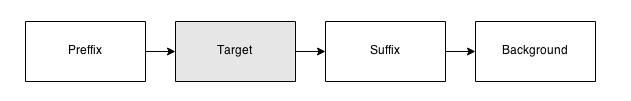
\includegraphics[width=0.8\linewidth]{./assets/images/zhang-hmm-ie}
    \center\footnotesize{Fonte: O próprio autor.}
\end{figure}

Os seguintes campos deveriam ser extraídos das informações dos restaurantes: \textit{restaurant name} (nome do restaurante), \textit{telephone number} (número de telefone), \textit{hours} (horas) e \textit{cuisine} (tipo de comida servida, como italiana, alemã, etc). Segundo Zhang \cite{Zhang-HMM-IE} os campos \textit{restaurant name} e \textit{telephone number} deveriam ser mais fáceis de serem obtidos, visto que o nome do restaurante geralmente se encontra em destaque, com alguma diferenciação visual. Já o telefone possui um formato numérico, que permite mais facilmente uma identificação de um padrão. O campo \textit{hours} também não seria complicado, embora se tenha uma variedade muito grande na representação desta informação. Já o campo \textit{cousine} foi mais difícil de ser extraído, visto a diversidade que existe na forma de um restaurante especificar e/ou representar sua cozinha, tanto na utilização de palavras diferentes quanto na própria identificação do estilo do restaurante por si só.

Como resultados esperados, os campos \textit{restaurant name} e \textit{telephone number} obtiveram muito êxito em sua extração, com resultados realmente consideráveis. Já os campos \textit{hours} e \textit{cousine} não tiveram resultados muito satisfatórios, o que pode ser explicado em função da característica dos HMMs de utilizar como modelo resultados de aprendizados anteriores, os \textit{training datasets}. Como nestes dois campos há uma grande possibilidade de representação, os resultados não foram tão eficazes, o que poderia ser resolvido com uma alteração no modelo HMM que permitisse que as palavras identificadas como sendo do campo \textit{cousine} fossem capturadas de maneira mais proveitosa, que estão, neste modelo sugerido, isoladas no estado \textit{Background}.

Em função dos resultados obtidos, pode-se considerar a performance do HMM na extração de informação como positiva, visto as possibilidades de variação do modelo, que permite um resultado mais preciso e próximo dos objetivos reais \cite{Zhang-HMM-IE}. Além disso, a utilização de resultados passados garante um aprendizado importante para que o modelo seja estabelecido, o que garante ainda mais um ganho de eficiência na aplicação desta técnica.

Além da utilização de HMM de forma natural, algumas variações de seu algoritmo são também citadas na literatura, como é o caso dos MEMMs (\textit{Maximum Entropy Markov Models}) \cite{maximum-entropy}. Nos MEMMs cada estado possui um modelo exponencial que utiliza as características de observação como entrada de dados (\textit{input}) \cite{Lafferty-CRF}. Estes modelos são baseados na técnica de HMM, se diferenciando na maneira como os estados se relacionam, bem como a relação entre suas transições, levando a citações independentes por alguns autores, porém, com herança conceitual dos modelos HMM.

\subsubsection{Word Clustering}
\label{sssec:word-clustering}

Técnicas de classificação de texto geralmente utilizam palavras extraídas como a principal fonte de recursos para a representação. Por outro lado, os \textit{clusters} de palavras tem sido uma proposta eficaz para a redução da dimensionalidade e da dispersão, melhorando assim a performance desta classificação \cite{Han-Giles-WC}.

O conceito de \textit{clusters} compreende um conjunto de palavras que formam um banco de dados de domínio (\textit{domain database}), que é aliado a um conjunto de propriedades ortográficas de palavras dentro do contexto específico. A utilização destes \textit{clusters}, juntamente com outras técnicas, tem mostrado um ganho de 6,6\% na performance de classificação de elementos de um cabeçalho de artigo científico, e ainda 8,4\% de ganho de performance para a extração das referências destes documentos \cite{Han-Giles-WC}.

A utilização destes grupos de palavras demonstra uma relação entre textos semelhantes dentro de um determinado contexto, permitindo que a extração dos metadados ocorra de maneira natural, com resultados mais eficazes.

Sendo assim, Han et al. apresentaram uma ideia de um \textit{cluster} de palavras para promover a extração de metadados de artigos científicos da área de Ciência da Computação, indo de maneira contrária às propostas mais tradicionais, que se baseiam, geralmente, apenas na ocorrência e estatísticas de palavras isoladas dentro do texto original.

Han et al. agruparam bases de dados de domínios diversos incluindo também propriedades ortográficas de palavras, com base em um conhecimento prévio de classes específicas, como autor, título, etc. Deste modo, palavras encontradas nos documentos vão sendo comparadas com palavras deste \textit{cluster}, permitindo identificar, por grupos, características semelhantes de metadados. Para cada classe (metadado) cria-se um \textit{cluster}, com suas palavras e propriedades ortográficas específicas.

Como exemplo, a palavra ``Mary'' faz parte do \textit{cluster} de ``nomes''. Portanto, existe uma probabilidade maior de ela, juntamente com seu grupo de palavras ao redor, fazer parte da classe ``autor'', por exemplo. Esta lógica é apresentada também para outras classes, como ``e-mail'' por exemplo, que pode ser identificado com a presença do caractere ``@'', levando à utilização de expressões regulares para encontrar padrões de ocorrências (\autoref{sssec:regular-expressions}).

\begin{figure}
    \centering
    \caption{\emph{Workflow} da extração de metadados usando \textit{cluster} de palavras.}
    \label{fig:workflow-rule-based}
    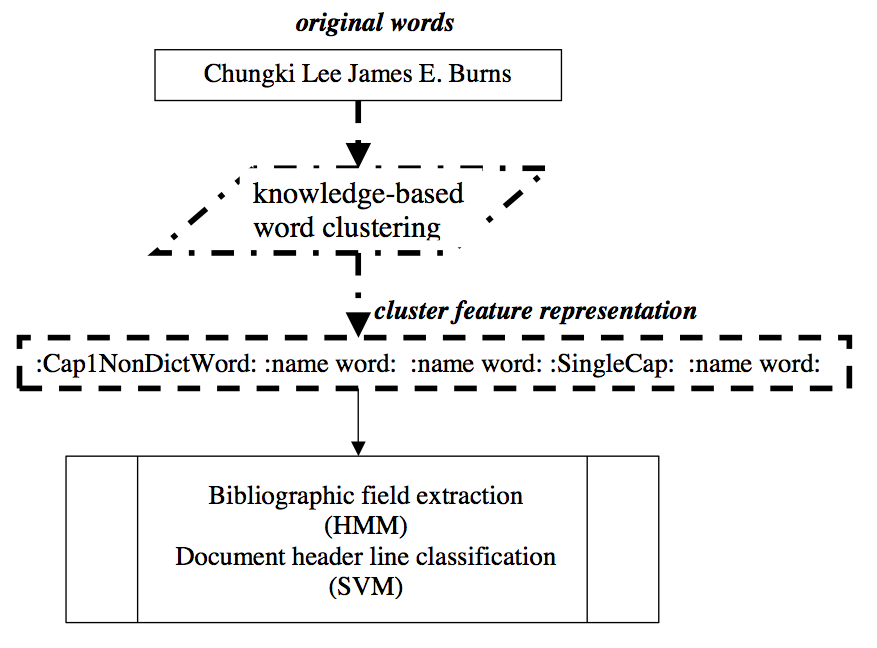
\includegraphics[width=0.7\linewidth]{./assets/images/workflow-rule-based}
    \center\footnotesize{Fonte: \cite{Han-Giles-WC}}
\end{figure}

A utilização de \textit{word clustering} possui um custo computacional muito baixo, o que pode ser considerado uma vantagem sobre demais técnicas computacionais \cite{Han-Giles-WC}.

Han et al. ainda utilizam da técnica de SVM (\autoref{sssec:svm}) para classificação de linhas de um cabeçalho de um documento, tanto em função dos bons resultados obtidos, quanto também pela boa performance apresentada. Deste modo, cada linha obtida se transforma em um vetor de palavras, que é comparado com seu respectivo \textit{cluster}, melhorando os resultados de classificação, unindo as duas técnicas em prol do mesmo objetivo.

A técnica de \textit{Word Clustering} se resume em 3 (três) etapas. A primeira compreende a construção das bases de dados, como referenciado por Han \cite{Han-SVM}, onde foram utilizadas também bases externas - nomes de estados americanos, países, cidades, nomes de dicionários, nomes de pessoas, códigos postais, etc -, unindo também bases construídas dentro de um domínio específico, como palavras pertencentes a uma classe específica.

A segunda etapa é chamada de \textit{Cluster Design}. Nesta etapa os \textit{clusters} são arquitetados, contemplando também propriedades ortográficas das palavras, formando então o dicionário com base nas características apresentadas.

Já a terceira etapa é chamada de \textit{Rule Design}, que consiste na combinação de palavras em diferentes domínios, nas suas verificações ortográficas e na classificação delas em seu \textit{cluster} correto. Por exemplo, nomes devem começar com a primeira letra maiúscula para então serem classificadas como pertencentes ao \textit{cluster} ``nomes''.

Além disso, foi observada também a presença de certas palavras que faziam parte de diversos \textit{clusters} ao mesmo tempo, o que permitiu que elas fossem classificadas em seu próprio grupo de palavras, tornando-se então independentes.

A representação através de \textit{clusters}, utilizada por Han et al. \cite{Han-Giles-WC}, conseguiu reduzir um texto original de 11.223 palavras em um \textit{cluster} de 588 elementos, permitindo ainda que ele fosse distribuído entre classes distintas, o que tornou o processo muito menos trabalhoso, porém mais eficaz.

Como resultado, a utilização desta técnica de clusterização permitiu um ganho considerável de performance, além de contribuir para uma precisão maior dos resultados, visto que são apresentados dentro de um domínio específico, perfazendo um contexto mais definido e com resultados mais garantidos.

Por outro lado a utilização desta técnica possui uma falha na semântica dos dados. No momento da classificação de classes, na separação e criação dos \textit{clusters}, por exemplo, um dígito ou conjunto deles é substituído pela identificação \texttt{:number:}. Isso faz com que ele se torne apenas um número qualquer, sem uma semântica específica, ou seja, pode ser tanto uma referência a alguma página do documento ou até mesmo um mês ou ano, por exemplo.


\subsubsection{Conditional Random Fields (CRFs)}
\label{sssec:crf}

% Falar sobre CRFs 

CRFs é um framework proposto por Lafferty et al. \cite{Lafferty-CRF} criado para construir modelos probabilísticos e dados marcados em sequência (\textit{label sequence data}), geralmente utilizados no reconhecimento de padrões e aprendizado de máquina (\textit{machine learning}).

Esta técnica oferece algumas vantagens se comparada com técnicas mais tradicionais, como HMM (\autoref{sssec:hmm}), se destacando a habilidade de diminuir pressupostos independentes feitos nestes modelos \cite{Lafferty-CRF}.

Modelos baseados em HMM possuem uma fraqueza, que é o problema denominado \textit{bias problem}. As transições de um estado somente competem entre elas, e não com todas as transições presentes no modelo. Elas são feitas com base probabilística de acordo com o estado inicial e a sequência de observação (\textit{observation sequence}).

Desta forma, devido ao \textit{bias problem}, em um caso extremo, um estado que tiver como opção de transição somente um outro estado, pode simplesmente ignorar a sequência de observação, o que traria efeitos contrários aos objetivos do processo inicial.

Lafferty et al. realizam comparações funcionais e práticas entre CRFs, HMM e MEMM (\textit{Maximum Entropy Markov Models}), uma variação da técnica de HMM, detalhada na \autoref{sssec:hmm}. A importante diferença entre CRFs e MEMMs é que MEMM utiliza modelos exponenciais como probabilidade de ocorrência de um próximo estado, enquanto a técnica de CRF possui um modelo exponencial único para toda a sequência de \textit{labels}, com base na sequência de observação. Segundo Lafferty et al. \cite{Lafferty-CRF} pode-se pensar na CRF como um modelo de estado finito sem normalização das probabilidades de transição.

Uma das vantagens de se utilizar CRFs sobre HMM é que ela absorve boa parte de suas qualidades, mas com a particularidade de resolver o \textit{bias problem}. Outra grande vantagem sobre HMMs e MEMMs é que a CRF possui resultados melhores quando a distribuição dos dados possui grande dependência do modelo, o que geralmente ocorre em casos mais práticos.

Um exemplo para entender o \textit{bias problem} foi também apresentado por Lafferty et al. \cite{Lafferty-CRF}. Ele propõe um modelo cujo objetivo é distinguir duas palavras: \texttt{rib} e \texttt{rob}, tendo como sequência de observação as letras \texttt{r i b}. O problema é identificado quando uma das duas palavras é mais comum no \textit{training set}, o que acarreta nas transições do estado inicial preferirem suas transições correspondentes, o que acaba sempre na vitória da palavra relacionada àquele estado.

Visando a comprovação e reconhecimento da eficiência da técnica de CRF na extração de informação foram aplicados dois tipos de experimentos:

\begin{enumerate}
    \item Verificação direta do \textit{bias problem};
    \item Geração de dados utilizando HMM aleatórios.
\end{enumerate}

Os resultados apontam que HMMs superam MEMMs em virtude do \textit{bias problem}. Por sua vez os CRFs superam os HMMs, sendo então considerada a melhor técnica para ser empregada com base no \textit{training set} utilizado \cite{Lafferty-CRF}. Outro ganho apresentado pode ser verificado ao agregar algumas características ortográficas à utilização de CRFs, aumentando o poder destes modelos condicionais.

De modo geral as CRFs utilizam a mesma lógica que modelos baseados em Markov (HMMs e MEMMs), se diferenciando nos aspectos probabilísticos para com as transições entre os estados, acarretando em resultados comparativamente melhores. Por corresponder a uma ``máquina'' de estado finito, a técnica é muito aplicável para funções de classificação sequencial, o que permite que seja treinada para se obter os melhores resultados probabilísticos \cite{Peng-CRF-IE}. Nas CRFs as transições de estado são também representadas como \emph{features} por alguns autores.

%Esta técnica é comparada e quase sempre utilizada juntamente com a HMM (Hidden Markov Models), de maneira a possuir algumas vantagens sobre esta última, como a habilidade de relacionar pressupostos independentes nos modelos, ou seja, relacionar observações e/ou interpretações.

Uma outra vantagem da técnica de CRFs - assim como dos modelos \emph{maximum entropy} - é que eles permitem o uso de características arbitrárias nos dados de entrada. As CRFs são utilizadas também em marcação e classificação de dados sequenciais, como linguagem natural, sequências biológicas (como os genes) ou estados computacionais.

% Falar sobre o uso de CRFs na extração de informação

Sua aplicação na extração de metadados foi apresentada por Peng et al. \cite{Peng-CRF-IE}, como uma maneira eficaz de extrair metadados em cabeçalhos e referências de artigos científicos. Deste modo, através da identificação destes padrões sequenciais pode-se determinar os tipos de dados existentes e então identificá-los, seguindo uma lógica/ordem pré-determinada.

Peng et al. apresentam resultados desta extração utilizando Conditional Random Fields (CRF) e aponta também algumas questões acerca da utilização testa técnica para este tipo de atividade. Os autores comparam as CRFs com técnicas de HMM (\autoref{sssec:hmm}) e SVM (\autoref{sssec:svm}), mencionando que a forma de trabalhar com CRF aponta parte das vantagens destas duas técnicas, destacando a junção entre as sequências e características dependentes, mas ao mesmo tempo arbitrárias. Ainda assim, segundo os autores, a utilização de CRFs para a tarefa de extração de metadados - ao se comparar com as demais técnicas de SVM e HMM - possui melhoras significativas.

Os autores definem quatro diferentes transições de estado para diferentes classes, em ordem diferente das técnicas derivadas de Markov (HMM):

\begin{enumerate}
    \item \emph{\textbf{First-order:}} os dados de entrada são examinados no contexto de somente um estado;
    \item \emph{\textbf{First-order + transitions:}} são adicionados alguns parâmetros correspondentes às transições;
    \item \emph{\textbf{Second-order:}} as entradas são examinadas no contexto dos estados atual e anterior;
    \item \emph{\textbf{Third-order:}} os dados de entrada são examinados no contexto do estado atual e de dois estados anteriores.
\end{enumerate}

Para a extração destes dados Peng et al. também consideram como sendo o cabeçalho de um artigo como sendo a parte inicial do documento até a introdução, ou somente a primeira página, o que ocorrer primeiro. Além disso, os autores consideram como os campos a serem analisados os mesmos 15 (quinze) que foram definidos anteriormente por Seymore et al. \cite{Seymore-HMM-IE}.

Para extração dos metadados dos cabeçalhos foi utilizado um \emph{dataset} com 935 (novecentos e trinta e cinco) documentos. Destes, 500 (quinhentos) foram utilizados para compor o \emph{training set} e os outros 435 (quatrocentos e trinta e cinco) para fins de teste, unicamente. Já do \emph{dataset} utilizado para extração das referências foram analisados 500 (quinhentos) documentos, dos quais 350 (trezentos e cinquenta) foram utilizados para o \emph{training set} e os demais 150 (cento e cinquenta) também para testes.

Para fins de resultados comparativos foram utilizadas três métricas:

\begin{enumerate}

    \item \emph{\textbf{Overall word accuracy:}} é uma métrica que utiliza a porcentagem de palavras das quais os nomes (\emph{labels}) previstos são exatamente seus valores reais. Esta métrica favorece aqueles campos que possuem muitas palavras, como, por exemplo, a introdução (\emph{abstract});

    \item \emph{\textbf{Average F-measure (F1):}} esta métrica se baseia na exatidão das ocorrências, considerando tanto a precisão quanto a memória de todos os campos (\emph{fields}). Esta métrica favorece campos com poucas palavras, visto sua característica mais importante, de focar na exatidão dos resultados.
    
    \item \emph{\textbf{Whole instance accuracy:}} nesta métrica uma ``instância'' é considerada como sendo todo um cabeçalho ou referência, de maneira integral. Desta forma esta métrica utiliza-se da porcentagem de instâncias das quais cada palavra é corretamente associada.

\end{enumerate}

Conforme pode-se observar na \autoref{tab:crf-results-headers} e \autoref{tab:crf-results-references} a utilização de CRFs para extração de metadados - tanto de cabeçalhos como de referências - teve resultados melhores do que a utilização de HMM (\autoref{sssec:hmm}), aumentando a performance em praticamente todos os campos, chegando a uma precisão de 98,3\% (\emph{overall accuracy}).

Pode-se observar também que a utilização de modelos HMM para precisão de palavras (campos com poucas palavras, onde a precisão é muito mais importante) é, de modo geral, pior do que quando utiliza-se de SVMs (coluna F1 da \autoref{tab:crf-results-headers}). Por outro lado, no campo \emph{abstract} HHM possui performance bem melhor que quando utilizado SVM (98\% contra 93,8\%).

\begin{table}
    \caption{Resultados de extração para CRFs após análise do \emph{dataset} com cabeçalhos \cite{Peng-CRF-IE}.}
    \begin{center}
        \begin{tabular}{|c|c|c|c|c|c|c|} \hline             
             & \multicolumn{2}{c|}{HMM} & \multicolumn{2}{c|}{CRF} & \multicolumn{2}{c|}{SVM} \\  \hline 
            Overall acc. & \multicolumn{2}{c|}{93.1\%} & \multicolumn{2}{c|}{\textbf{98.3\%}} & \multicolumn{2}{c|}{92.9\%} \\ \hline
            Instance acc. & \multicolumn{2}{c|}{4.13\%} & \multicolumn{2}{c|}{\textbf{73.3\%}} & \multicolumn{2}{c|}{-} \\ \hline \hline
             & acc. & F1 & acc. & F1 & acc. & F1 \\ \hline
            Title & 98.2 & 82.2 & 99.7 & \textbf{97.1} & 98.9 & 96.5 \\ \hline
            Author & 98.7 & 81.0 & 99.8 & \textbf{97.5} & 99.3 & 97.2 \\ \hline
            Affiliation & 98.3 & 85.1 & 99.7 & \textbf{97.0} & 98.1 & 93.8 \\ \hline
            Address & 99.1 & 84.8 & 99.7 & \textbf{95.8} & 99.1 & 94.7 \\ \hline
            Note & 97.8 & 81.4 & 98.8 & \textbf{91.2} & 95.5 & 81.6 \\ \hline
            Email & 99.9 & 92.5 & 99.9 & \textbf{95.3} & 99.6 & 91.7 \\ \hline
            Date & 99.8 & 80.6 & 99.9 & \textbf{95.0} & 99.7 & 90.2 \\ \hline
            Abstract & 97.1 & 98.0 & 99.6 & \textbf{99.7} & 97.5 & 93.8 \\ \hline
            Phone & 99.8 & 53.8 & 99.9 & \textbf{97.9} & 99.9 & 92.4 \\ \hline
            Keyword & 98.7 & 40.6 & 99.7 & \textbf{88.8} & 99.2 & 88.5 \\ \hline
            Web & 99.9 & 68.6 & 99.9 & \textbf{94.1} & 99.9 & 92.4 \\ \hline
            Degree & 99.5 & 68.8 & 99.8 & \textbf{84.9} & 99.5 & 70.1 \\ \hline
            Pubnum & 99.8 & 64.2 & 99.9 & 86.6 & 99.9 & \textbf{89.2} \\ \hline
            \hline
            Average F1 & & 75.6 & & \textbf{93.9} & & 89.7 \\ \hline
        \end{tabular}
    \end{center}
    \label{tab:crf-results-headers}
\end{table}

\begin{table}
    \caption{Resultados de extração para CRFs após análise do \emph{dataset} com referências \cite{Peng-CRF-IE}.}
    \begin{center}
        \begin{tabular}{|c|c|c|c|c|} \hline             
             & \multicolumn{2}{c|}{HMM} & \multicolumn{2}{c|}{CRF} \\  \hline 
            Overall acc. & \multicolumn{2}{c|}{85.1\%} & \multicolumn{2}{c|}{\textbf{95.37\%}} \\ \hline 
            Instance acc. & \multicolumn{2}{c|}{10\%} & \multicolumn{2}{c|}{\textbf{77.33\%}} \\ \hline \hline
             & acc. & F1 & acc. & F1 \\ \hline 
            Author & 96.8 & 92.7 & 99.9 & \textbf{99.4} \\ \hline 
            Booktitle & 94.4 & 0.85 & 97.7 & \textbf{93.7} \\ \hline 
            Date & 99.7 & 96.9 & 99.8 & \textbf{98.9} \\ \hline 
            Editor & 98.9 & 70.8 & 99.5 & \textbf{87.7} \\ \hline 
            Institution & 98.5 & 72.3 & 99.7 & \textbf{94.0} \\ \hline 
            Journal & 96.6 & 67.7 & 99.1 & \textbf{91.3} \\ \hline 
            Location & 99.1 & 81.8 & 99.3 & \textbf{87.2} \\ \hline 
            Note & 99.2 & 50.9 & 99.7 & \textbf{80.8} \\ \hline
            Pages & 98.1 & 72.9 & 99.9 & \textbf{98.6} \\ \hline
            Publisher & 99.4 & \textbf{79.2} & 99.4 & 76.1 \\ \hline
            Tech & 98.8 & 74.9 & 99.4 & \textbf{86.7} \\ \hline
            Title & 92.2 & 87.2 & 98.9 & \textbf{98.3} \\ \hline
            Volume & 98.6 & 75.8 & 99.9 & \textbf{97.8} \\ \hline
            \hline
            Average F1 & & 77.6\% & & \textbf{91.5\%} \\
            \hline
        \end{tabular}
    \end{center}
    \label{tab:crf-results-references}
\end{table}

Com base nos resultados apresentados pode-se considerar que o trabalho de Peng \cite{Peng-CRF-IE} contribuiu para o estado da arte, melhorando a performance na extração de metadados em artigos científicos. Assim, a utilização de CRFs mostra-se muito eficaz por reduzir consideravelmente os erros encontrados, aumentando o sucesso da aplicação desta técnica neste contexto.

\section{Trabalhos Correlatos}
\label{sec:revision}

% Falar aqui sobre os estudos de comparações de Granitizer

Técnicas de \emph{machine learning} não são novas, porém suas aplicações são inúmeras. Estas técnicas inicialmente eram utilizadas apenas para classificação de palavras e processamento de linguagem natural, mas foram sendo utilizadas em diversas outras áreas resolvendo problemas distintos e inovando em soluções, como é o caso da extração de informação.

O aperfeiçoamento da aplicação destas técnicas para a área de extração de informação acarretou em um resultado muito positivo, melhorando a precisão dos resultados obtidos. Assim, algoritmos foram/são alterados e otimizados visando obter maiores performances e resultados cada vez melhores.

Pode-se perceber que cada técnica de classificação e/ou extração de informação possui suas particularidades e características diferentes. Assim, é possível notar, em grande parte, que algumas possuem uma melhor aplicação para extração de determinado campo, ou conjunto deles. Pequenas modificações são necessárias para que todo o contexto de um artigo científico seja mapeado com sucesso, sendo às vezes necessária a utilização de diversas técnicas em um único projeto.

Para isso, diversas comparações entre técnicas foram feitas. Algumas - inclusive já mencionadas ao longo deste capítulo - foram feitas quando do surgimento de uma nova técnica, onde esta era comparada com técnicas anteriores. Porém, este tipo de comparação torna-se tendenciosa, visto que os campos analisados, bem como os \emph{datasets} utilizados, tendenciam para resultados positivos da nova técnica apresentada. Além disso, geralmente os \emph{datasets} utilizados são focados em documentos da área de Ciência da Computação, e tendem a seguir um padrão visual já estipulado pelos grandes eventos da área.

Em função deste problema alguns autores realizam comparações de técnicas, isoladamente ou com utilização de ferramentas, para analisar um grupo de documentos reais, objetivando um resultado mais próximo da realidade e, consequentemente, mais passível de erros. Estas comparações são relevantes para o Estado da Arte deste trabalho.

Granitzer et al. \cite{Granitzer-2012-LayoutBased} comparam o uso de Conditional Random Fields (\autoref{sssec:crf}) e Support Vector Machines (\autoref{sssec:svm}) na extração de metadados em artigos científicos. Para isso são utilizados \emph{datasets} multidisciplinares, como \emph{Mendeley} e \emph{e-Prints}, que fazem parte de um grupo social de \emph{datasets}, permitindo uma contribuição global entre pesquisadores de diversas áreas do conhecimento.

Em virtude da existências destes repositórios a informação fica cada vez mais descentralizada e, portanto, são necessários cada vez mais mecanismos inteligentes para garantir a alta qualidade dos metadados extraídos \cite{Granitzer-2012-LayoutBased}. A combinação destes mecanismos com pós-processamento inteligente contribui para o processo, elevando a qualidade do resultado final encontrado.

% CiteSeer e Mendeley utilizam SVMs. Granitzer 2012

Visando um reconhecimento maior dos resultados obtidos, Granitzer et al. realizam comparações dos resultados com a aplicação de três ferramentas: ParsCit (\autoref{ssec:parscit}), Mendeley Desktop (\autoref{ssec:mendeley}) e sua própria ferramenta baseada em CRFs, no qual se referem como ``Layout-based CRF''.

Este trabalho \cite{Granitzer-2012-LayoutBased} é uma continuação do trabalho anteriormente realizado \cite{Granitzer-2012-Crowdsourced}, onde as ferramentas Mendeley Desktop (\autoref{ssec:mendeley}) e ParsCit (\autoref{ssec:parscit}) foram comparadas, utilizando, porém, um \emph{dataset} menor. Desta vez foi incluída a técnica de Conditional Random Fields (CRF) na comparação que, de acordo com a literatura mencionada neste trabalho, possui resultados melhores do que a utilização de Hidden Markov Models (HMMs - \autoref{sssec:hmm}).

Foram analisadas 20.672 publicações do \emph{dataset} Mendeley, abrangendo diversas áreas do conhecimento como Ciência de modo geral, Ciência da Computação, Biomedicina e Física. Já no \emph{dataset} e-Prints foram analisadas 2.452 publicações de áreas como Física, Medicina e diversas outras pertencentes ao IEEE, ligadas geralmente à área de computação.

Foi relatado que uma das etapas principais para um bom processamento e uma boa precisão é o ``pós-processamento''. A aplicação de diversas análises (inclusive matemáticas) nos resultados extraídos garante um conjunto de dados de saída muito melhor e mais acurado. Segundo Granitzer et al. \cite{Granitzer-2012-LayoutBased} estas tarefas são de responsabilidade do setor de engenharia, onde diversos detalhes devem ser observados e diversos algoritmos aplicados.

De modo geral, os resultados obtidos pelas ferramentas Mendeley e ParsCit foram considerados ruins para os grupos pertencentes à área médica \cite{Granitzer-2012-LayoutBased}. Porém, estes resultados poderiam ser melhorados com um novo treino dos dados (\emph{training set}), com aplicações específicas para aquela área do conhecimento, no caso, a medicina. Outro ponto interessante observado foi o fato de a extração dos títulos ter ocorrido mais facilmente do que a extração dos autores, variando a performance dos resultados em função da técnica utilizada.

Para os outros grupos os resultados foram bem positivos, observando uma pequena diferença entre os números obtidos com as ferramentas Mendeley e ParsCit, que foram muito superiores aos resultados da implementação CRF dos autores. Isso se deve ao fato das duas ferramentas anteriores utilizarem de pós-processamento dos dados, o que garantiu aos resultados obtidos uma precisão muito maior \cite{Granitzer-2012-LayoutBased}.

De acordo com Granitzer et al., mesmo a técnica de CRF possuindo melhores modelos de extração de informação, foi-se observado que a técnica de SVM utilizada pelo Mendeley Desktop supera a CRF no que tange extração de metadados \cite{Granitzer-2012-LayoutBased}.

A ferramenta ParsCit de modo geral não teve resultados melhores que o Mendeley Desktop. Para a área de Ciência da Computação, mais especificamente na base de dados do IEEE, ambas as ferramentas obtiveram excelentes resultados. Já na base de dados da ACM o Mendeley obteve melhores resultados do que o ParsCit \cite{Granitzer-2012-LayoutBased}.

\section{Ferramentas de Extração de Metadados}
\label{sec:environments}

Algumas ferramentas fundamentam suas funcionalidades de extração em padrões pré-definidos, identificando dados relevantes dentro de uma região específica dos artigos, o que facilita a procura e consequentemente aumenta a velocidade nos resultados finais.

Estas ferramentas geralmente permitem uma variedade muito grande de leiautes, embora nem todos já estejam previamente definidos. Geralmente suporte a novos leiautes são inseridos em novas versões ou até mesmo por contribuições das mais diversas, como é o caso dos projetos de código livre, os chamados projetos \textit{open source}.

Abaixo segue uma relação das principais ferramentas relacionados à área de extração de metadados em artigos científicos, com informações sobre sua história, funcionamento e algumas técnicas que utilizam.

\subsection{Cermine}
\label{ssec:cermine}

% CERMINE

Uma destas ferramentas é o recente Cermine \cite{cermine}, uma biblioteca \textit{open source} desenvolvida na linguagem de programação Java que permite que sejam extraídos os metadados de artigos científicos em formato digital PDF, oferecendo ainda a possibilidade de cruzamento de dados por meio de referências e títulos, permitindo assim identificar citações bem como a relevância de um determinado documento.

O Cermine ainda possui um mecanismo de aprendizagem próprio que permite que, na medida que dados forem sendo alterados, ele consiga absorver os detalhes passados e realizar mudanças em sua forma de realizar a extração. Deste modo ele permite adaptações para novos padrões de leiautes, o que permite de maneira geral que uma grande gama de modelos seja então abrangida. 

Seu grande diferencial em comparação com as demais ferramentas é que ele não somente extrai os metadados de um artigo, mas também analisa todo o seu conteúdo, incluindo citações a outros documentos, que podem ser facilmente cruzados por meio de informações como título e autor(es).

Seu mecanismo considera arquivos PDF em forma textual, sem a utilização de imagens. A ferramenta considera regiões, linhas e páginas como pontos estratégicos para a extração de informações. As bases destas regiões possuem padrões que são utilizados juntamente com técnicas de SVM \cite{Han-SVM} (detalhado na \autoref{sssec:svm}). Dessa forma seu mecanismo condensa um leiaute onde as informações geralmente estão dispostas, permitindo aferir que em um determinado local do arquivo estejam o título e o nome dos autores, por exemplo. 

Com estas regiões definidas o Cermine extrai as informações com base em padrões preestabelecidos, gerando resultados para os metadados e referências encontradas. O formato de saída dos resultados é no formato XML, permitindo que possam ser compartilhados com outros sistemas por possuir uma leitura semântica e ao mesmo tempo fácil de ser interpretada pelas linguagens de programação. A \autoref{fig:cermine-workflow} demonstra como o processo de extração do Cermine funciona.

\begin{figure}
    \centering
    \caption{Cermine Extraction Workflow}
    \label{fig:cermine-workflow}
    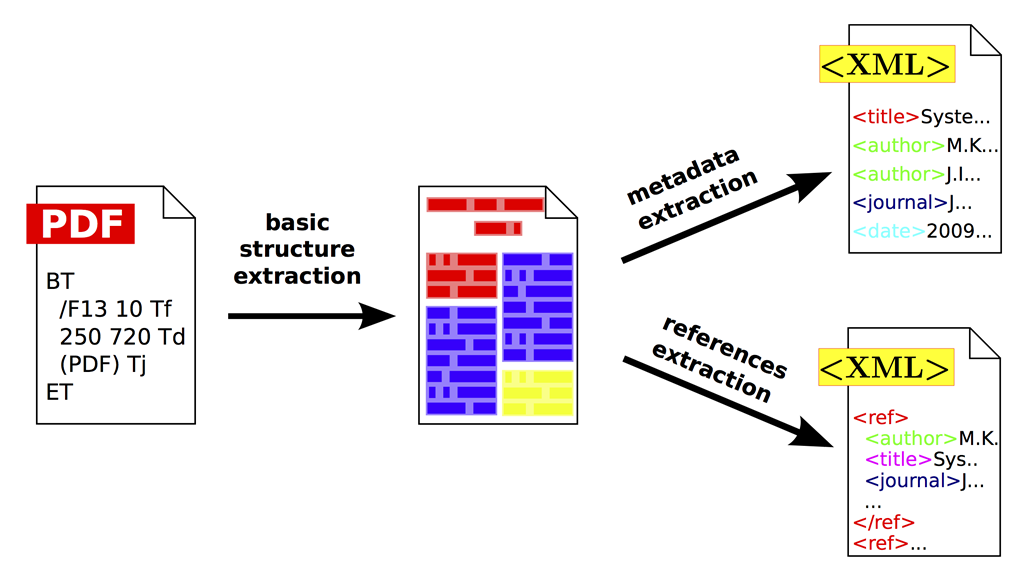
\includegraphics[width=0.7\linewidth]{./assets/images/cermine}
    \center\footnotesize{Fonte: \cite{cermine}}
\end{figure}

Após o mapeamento definido a ferramenta identifica regiões de acordo com seu conteúdo de entrada, as quais ele chama de \textit{zones}. Estas regiões são determinadas a fim de extrair suas informações mais relevantes, separando, por exemplo, a área destinada aos metadados do arquivo. O Cermine divide estas \textit{zones} da seguinte maneira:

\begin{itemize}

    \item \textbf{Metadata:} É a região mais ao alto do documento, onde obtém os metadados, que seriam o resumo, \textit{bib\_info}, tipo, título, afiliação, autores, datas, editores e palavras-chaves.

    \item \textbf{References:} Região responsável por identificar detalhes de referências que foram utilizadas no artigo, como título e autores, por exemplo.

    \item \textbf{Body:} O texto geral do artigo, incluindo equações, imagens e tabelas.

    \item \textbf{Other:} Outros detalhes menos significantes semanticamente, como número das páginas, dentre outros dados.

\end{itemize}

A extração das referências abrange também seus próprios metadados. Tanto no texto corrido (\textit{Body}) quanto na lista de referências do documento o \textit{parser} do Cermine analisa o conteúdo linha a linha, permitindo uma extração de dados mais eficaz. Das referências são extraídos os seguintes dados: autor, título, nome do \textit{journal}, volume, \textit{issue}, páginas, \textit{publisher}, localização e ano.

\subsection{TeamBeam}
\label{ssec:teambeam}

Outra ferramenta de destaque é o TeamBeam \cite{teambeam}, cuja base ideológica possui objetivos bem sociais, de contribuir com o compartilhamento de conhecimento. Basicamente o objetivo do projeto é extrair metadados de artigos científicos, porém focado apenas nestes, de maneira a extrair título, nome do \textit{journal}, resumo e informações sobre os autores, como nome, endereço de e-mail e afiliações.

O projeto também é de código livre (\textit{open source}) e é baseado na extração de pequenos blocos de texto. A manipulação dos arquivos PDF é feita pela biblioteca PDFBox\footnote{Biblioteca de manipulação de arquivos PDF mantida pela Fundação Apache. Disponível em \url{https://pdfbox.apache.org/}}, que fornece meios eficazes de extrair textos com base nas regiões desejadas.

O TeamBeam utiliza o algoritmo de \textit{Maximum Entropy} \cite{maximum-entropy}, que utiliza basicamente de tarefas de classificação sequencial como ferramenta principal para obtenção de padrões. A base deste algoritmo está na utilização de CRFs (\autoref{sssec:crf}), principalmente no que diz respeito à extração dos metadados \cite{Peng-CRF-IE}.

O processo de extração é feito basicamente em duas etapas. A primeira é a etapa de classificação de blocos de texto (\textit{text block classification}), onde geralmente já é possível obter algum dado concreto como resultado. Nesta etapa o objetivo é associar certos blocos de texto a um dos seguintes marcadores: \textit{Title Block}; \textit{Sub-Title Block}; \textit{Journal Block}; \textit{Abstract Block}; \textit{Author Block}; \textit{E-Mail Block}; \textit{Affiliation Block}; \textit{Author-Mixed Block}; e \textit{Other Block}.

Dependendo do leiaute do artigo alguns metadados podem vir divididos em blocos de texto diferentes, necessitando de um processamento posterior, como é o caso, geralmente, dos blocos com informações sobre os autores. Neste caso também é realizada a etapa de classificação de token (\textit{token classification}), que se resume na classificação de palavras individualmente de acordo com um dos seguintes marcadores: \textit{Given Name}; \textit{Middle Name}; \textit{Surname}; \textit{Index}; \textit{Separator}; \textit{E-Mail}; \textit{Affiliation-Start}; \textit{Affiliation}; e \textit{Other}.

Kern et al. defendem a ideia de excelentes resultados do TeamBeam ao ser comparado com outros projetos. Este fato é dado em virtude das características que são levadas em consideração no processamento da ferramenta, utilizando de dicionários, informações de leiaute e modelos de linguagem.

A fim de analisar os resultados obtidos com a aplicação das técnicas descritas no TeamBeam, os autores comparam as técnicas utilizadas com outras técnicas de outras ferramentas, que utilizam processos diferentes de análises.

Para fins de comparação de resultados, os autores citam as ferramentas ParsCit (\autoref{ssec:parscit}) e Mendeley Desktop (\autoref{ssec:mendeley}). Como conclusão ele compara estas três ferramentas separadamente, por não abrangerem todos os detalhes que o TeamBeam possui, o que tornaria a comparação desleal.

Assim, ele chega à conclusão que em virtude das diferentes formas de processamento dos dados feitas por cada umas das ferramentas, chega-se a resultados mais precisos para cada campo extraído. As ferramentas baseadas em dicionário apresentam melhores resultados para extração de autores, visto que baseiam-se em \textit{data-sets\footnote{Bases de dados com nomes dos autores mais citados e outras informações já catalogadas que são armazenadas para consulta pública.}} já consolidados.

\subsection{Mendeley}
\label{ssec:mendeley}

Mendeley é um dos projetos mais complexos e completos que existem na atualidade. Além de uma poderosa ferramenta na extração de metadados o projeto se transformou em uma plataforma completa para pesquisadores. Sua pesquisa se iniciou em novembro de 2007 por três estudantes alemães de doutorado, tendo sua primeira versão lançada em agosto de 2008. Em 2013 o projeto foi vendido para uma empresa, que passou a liderar o processo de criação e desenvolvimento. Atualmente o Mendeley é um projeto amplo, porém estritamente comercial, que possui uma plataforma de pesquisa e gestão de documentos como seu principal produto ofertado.

Os serviços oferecidos possuem modalidades grátis e paga, de acordo com a necessidade de cada usuário. Assim como o CiteULike (\autoref{ssec:citeulike}) o projeto se tornou referência no meio acadêmico, sendo utilizado e comentado por diversos pesquisadores. Em virtude de seu objetivo comercial a ferramenta não possui código aberto atualmente, o que não permite seu uso sem ser através do serviço oferecido pela empresa.

A ferramenta pode ser utilizada via Web, como aplicativo \emph{desktop}, para \emph{tablets} ou \emph{smartphones}. Visto seu aspecto social e suas inúmeras funcionalidades o projeto se tornou uma rede social acadêmica, tanto do ponto de vista de organização de documentos até mesmo para interação entre pesquisadores. A ferramenta permite que usuários façam \emph{upload} de artigos em formato PDF para que sejam armazenados em sua biblioteca pessoal. Estes arquivos são analisados e seus metadados são extraídos e enviados para os servidores centrais da ferramenta.

Além de organizar sua biblioteca pessoal é possível também fazer anotações em documentos, destacar partes de texto, exportar citações, gerenciar documentos e compartilhar informações com outros pesquisadores, o que torna a plataforma extremamente completa e funcional.

A pesquisa iniciada pelos três estudantes de doutorado levou em consideração técnicas de \emph{machine learning} e \emph{metadata extraction}, como SVM, por exemplo \cite{Granitzer-2012-LayoutBased}. A ferramenta utiliza um modelo de SVM de dois estágios (\emph{two-stages SVM}) \cite{Han-SVM} no que tange a extração dos metadados, obtendo uma grande exatidão dos resultados.

Pela sua complexidade e por abranger uma gama de funcionalidades muito grande, s serviço foi comparado à rede Last.FM \cite{Mendeley-LastFM}. Assim como a rede social de música o Mendeley permite que o usuário organize sua biblioteca digital de pesquisa de maneira bem eficaz, podendo compartilhar, distribuir e realizar diversas outras funções, assim como é possível na plataforma musical Last.FM.

Por ser um serviço a bastante tempo no mercado o Mendeley funciona também como um grande \emph{dataset}, permitindo que parte de sua coleção de artigos seja utilizada para fins de pesquisa, assim como ocorre com o CiteULike (\autoref{ssec:citeulike}), por exemplo. Isso facilita muito a descoberta de novas ferramentas e técnicas pois permite que uma quantidade muito grande de documentos seja analisada de maneira semi-estruturada, gerando então novos conhecimentos na área.

Após a venda da plataforma o projeto teve seu foco muito mais voltado ao comercial, ao contrário do que era anteriormente. A utilização de seus dados ficou restrita e a geração de receita se transformou no principal objetivo da companhia, o que trouxe algumas desvantagens para a pesquisa livre como um todo.

Algumas das funcionalidades do Mendeley:

\begin{itemize}
    \item Multiplataforma, podendo funcionar tanto na Web como em Windows, Mac, Linux, iPhone e iPad;
    \item Extração de metadados de artigos em formato PDF (ponto de pesquisa deste trabalho);
    \item Centralização de sua biblioteca digital, sendo a mesma disponibilizada em qualquer plataforma, pois fica disponível na nuvem (\emph{cloud computing});
    \item Visualizador de PDF embutido, o que permite marcações em texto e inclusão de notas personalizadas;
    \item Pesquisa completa da base de dados dos artigos existentes;
    \item Inclusão de \emph{tags} nos documentos, permitindo uma categorização dos mesmos dentro da biblioteca pessoal de cada usuário;
    \item Permite que citações e bibliografias sejam exportas em formato Microsoft Word, LibreOffice e \LaTeX;
    \item Criação de grupos públicos e privados entre pesquisadores, permitindo compartilhamento de conteúdo entre os usuários;
    \item É uma Rede Social completa, permitindo \emph{posts}, comentários, páginas de perfil, etc;
    \item Provém uma série de estatísticas com base nos documentos pertencentes à sua biblioteca digital.
\end{itemize}

% Mendeley usa two-stages SVM method \cite{Han-SVM} e \cite{Granitzer-2012-LayoutBased}

Embora o sucesso do projeto seja muito grande e suas funcionalidades permitam uma série de funções a serem utilizadas pelos pesquisadores, em virtude do foco deste trabalho, o Mendeley se torna uma ferramenta pouco útil, visto que não possui o seu código aberto e não permite que seu código seja instalado em outras máquinas para que sua funcionalidade de extração de metadados seja testada em separado. Mesmo assim, o projeto é bastante promissor e garante uma gama de funções que todo pesquisador necessita, além de organizar de maneira bem eficaz os artigos e demais documentos que fazem parte de um bom trabalho de pesquisa.

\subsection{CiteULike}
\label{ssec:citeulike}

Uma outra ferramenta de destaque é o CiteULike \cite{citeulike} e pode ser acessada em \url{http://citeulike.org}. Ela é uma fusão de dois serviços: um serviço de \emph{bookmarking} via Internet, bem como também um sistema de gestão de referências bibliográficas. A união destas duas funcionalidades permitiu um compartilhamento muito grande de conhecimento entre pesquisadores, de modo a promover uma disseminação de informação com o envio de links contendo \emph{papers} de pesquisa. 

O projeto foi criado em 2004 por Richard Cameron, mas em 2006 a empresa Oversity Ltd. assumiu seu controle e manutenção \cite{CiteULike-FAQ}. O CiteULike pode ser acessado através de um navegador e fica disponível na Internet, de fácil acesso. O projeto ainda encontra-se ativo e em constante evolução, tanto por parte da equipe que o mantém, como por parte de seus usuários.

O projeto é livre desde seu lançamento e não tem nenhum custo para seus utilizadores. Seu objetivo inicial surgiu de um problema para busca de material bibliográfico. Deste modo o CiteULike foi criado para remover este espaço vazio entre pesquisadores, além de permitir que eles compartilhem bibliografias de maneira simplificada, podendo inclusive contribuir para grupos de pesquisa, por exemplo.

Um dos detalhes desta ferramenta é que ela funciona com base em fontes externas de dados. Quando um usuário encontra na Internet um artigo que lhe é interessante ele pode adicioná-lo à sua lista pessoal (\emph{bookmarking}). Assim, o CiteULike automaticamente visita este endereço informado e realiza uma extração de dados dos detalhes das citações do artigo, salvando o link para este \emph{paper} em sua base de dados \cite{citeulike}. Além disso, ele permite que os metadados deste artigo também sejam extraídos, como título, autores, \emph{journal name}, número de páginas, etc, com base no link fornecido, seguinte para tal o padrão visual daquele \emph{publisher}.

Como se pode ver, o CiteULike preserva a informação livre. Ele somente coleta \emph{papers} que já estão disponíveis na Internet, com base em um link fornecido por um usuário. Outro ponto de interesse é que a ferramenta também analisa informações de citação para que possa criar um link reverso para os \emph{papers} já analisados e existentes em sua base. Deste modo, de posse de um link para um determinado artigo o CiteULike consegue analisar quais outros artigos este artigo cita, permitindo criar uma rede de citações entre documentos, o que facilita a disseminação de conhecimento e permite que pesquisadores distintos possam usufruir deste conjunto de informações previamente analisadas.

Outro detalhe importante é o fato do projeto ser ao mesmo tempo um serviço social. Além do armazenamento destes artigos em forma de links, ao adicionar um artigo em sua lista pessoal, o usuário também pode associar \emph{tags} àquele artigo. Isso permite uma categorização muito particular e ainda permite que artigos sejam procurados bem facilmente com bases nestas \emph{tags} fornecidas. De certa forma, outros pesquisadores podem se beneficiar destas informações, pois elas funcionam como uma folksonomia específica para aquele determinado domínio, que pode ser de interesse de outros pesquisadores também. Outro detalhe importante de destaque do ponto social da ferramenta é que ela permite um sistema de votação nos artigos. Cada artigo pode ser votado por usuários, criando-se um ranking dos artigos mais interessantes, tendo um local de destaque na página inicial da ferramenta.

Um grande detalhe do CiteULike é que ele permite que suas informações sejam utilizadas para análise de dados futuros, permitindo assim uma evolução da área de \emph{machine learning} e \emph{metadata extraction}. Como o CiteULike cria uma rede de artigos, ao mesmo tempo ele possui um banco de dados muito rico, que pode se utilizado como um \emph{dataset} posteriormente, visto suas informações semi-estruturadas já existentes. Inclusive os autores citam o fato de já existirem diversos projetos independentes atualmente que utilizam o \emph{dataset} do CiteULike para realizar suas análises \cite{citeulike}. Atualmente, no momento da realização deste trabalho, na base de dados do CiteULike podemos encontrar mais de 7.900.000 (sete milhões e novecentos mil) artigos.

Como o banco de dados do CiteULike é criado de forma estruturada a disseminação de conhecimento entre os pesquisadores é facilmente realizada. De posse do link para um determinado artigo a ferramenta consegue todos os detalhes deste documento, como título, autores, etc. Assim permite-se uma pesquisa muito rica em um conjunto de metadados previamente extraídos, criando então uma rede de distribuição de artigos, contribuindo para a comunicação entre pesquisadores de modo geral.

O projeto cumpriu basicamente duas regras:

\begin{enumerate}
    \item Ele criou um modelo para coleta de informações que é de fácil entendimento para o usuário final, extraindo metadados relevantes que permitem criar automaticamente uma rede de conteúdo, sem deixar de apontar para o artigo em seu site original;
    \item Ele mudou a maneira tradicional de descobrir e compartilhar informação, visto que a ferramenta permite que usuários acessem suas listas pessoais entre si, disseminando conhecimento com base em um conhecimento já pré-definido por um pesquisador.
\end{enumerate}

Outro detalhe que permite um uso diferenciado do projeto é a formação de grupos de pesquisa. Com base em interesses similares no histórico de pesquisa, o CiteULike permite que pesquisadores sejam ligados, compartilhando temas semelhantes e informações de maneira precisa e direta.

Tecnicamente o CiteULike foi criado utilizando como banco de dados o PostgreSQL\footnote{Sistema de Banco de Dados relacional com tradição e excelente performance. Sua página inicial é \url{http://www.postgresql.org}.}, Tcl\footnote{Linguagem de programação de scripts muito utilizada em ambientes Linux. Pode ser acessada em \url{http://www.tcl.tk}.} como linguagem de programação e ainda utilizando Memcached\footnote{Sistema de cacheamento baseado em memória, que permite um ganho excelente de performance em ambientes Web, sendo uma das mais utilizadas nos dias atuais. Detalhes em \url{http://memcached.org}.} para criação de cache dos dados armazenados, o que aumentou (e muito) a performance da ferramenta. Seus servidores são baseados em Linux e backups são feitos de 15 em 15 minutos \cite{citeulike}.

Com base nesta quantidade de detalhes e vantagens o CiteULike se tornou um ponto de referência para catalogação e organização de artigos científicos, permitindo a contribuição entre pesquisadores e formando então uma rede de contribuição que favorece a disseminação da pesquisa ao redor do mundo.

\subsection{CiteSeer}
\label{ssec:citeseer}

Um dos projetos mais específicos encontrados é o CiteSeer \cite{citeseer} e pode ser acessado em \url{http://citeseerx.ist.psu.edu/}. Seu objetivo não é apenas extrair dados em artigos, mas sim também analisar citações de outros documentos no conteúdo textual encontrado. Assim, ele é capaz de identificar quais documentos são citados, quantas vezes são citados e onde são citados, se assemelhando muito ao processo de citação natural. O CiteSeer foi criado pelos pesquisadores Lee Giles, Kurt Bollacker e Steve Lawrence em 1997 e utiliza modelos SVM para extração de metadados com bastante eficácia \cite{Granitzer-2012-LayoutBased}.

Desta forma, com estas informações identificadas, ele consegue criar um \textit{ranking} dos documentos citados, incluindo seus autores e \textit{journals}, criando a partir de um documento fonte todo um conjunto de relações com outros documentos de uma maneira estatística bem eficaz.

Os índices de citações (\textit{citation indexes}), que são utilizados no projeto, foram originalmente criados para a recuperação de informação, porém sua utilidade é tamanha que permite que citações sejam indexadas de maneira eficaz, permitindo inclusive que referências de documentos em idiomas diferentes sejam identificadas. Desta maneira, essa técnica pode ser utilizada de diversas formas, não somente na identificação de citações, mas envolvendo também um conjunto de informações, como inclusive identificar a reputação de um determinado artigo científico no meio em que se encontra, simplesmente analisando onde é referência em relação ao número de vezes em que é citado.

Uma proposta interessante em que se baseia o CiteSeer é a de Cameron \cite{cameron}. Seu objetivo é de formar uma Base de Citações Universal, onde todos os artigos estariam ligados entre si, independente de qualquer fator externo, como idioma, por exemplo. A diferença entre esta proposta e o trabalho realizado com o CiteSeer é que este último permite que os documentos sejam analisados sem nenhum esforço extra, ou seja, sem a intervenção dos autores dos documentos, como é proposto por Cameron. Neste caso, os documentos seriam analisados de maneira automática, diminuindo o tempo necessário para o relacionamento de todos eles e aumentando a eficácia e eficiência do processo.

O funcionamento do CiteSeer é relativamente simples, porém o trabalho realizado por detrás do processo envolve muito estudo e dedicação. Basicamente ele é capaz de fazer o \textit{download} de \textit{papers} utilizando a Internet (como um coletor de artigos), convertê-los em texto e realizar a análise de todas as suas citações e metadados. Este resultado é armazenado em um banco de dados para consultas e relacionamentos futuros. Um dos pontos interessantes desta análise é que, como ela é feita com base em referência textual, identificados origem e destino, ela pode ser facilmente aplicada tanto no sentido natural de leitura (um artigo cita outros) quanto no sentido inverso (um artigo é citado por outros). 

O projeto também possui suas desvantagens, como por exemplo, a não cobertura de alguns \textit{journals} importantes, indexando todos seus documentos online e de maneira automática. Além disso o projeto original não é capaz de identificar mais de um autor nos documentos, sendo a identificação feita apenas pelo campo autor, tendo ele um ou mais pesquisadores envolvidos.

Basicamente o projeto analisa o documento em partes:

\begin{itemize}
    \item \textbf{URL:} a URL onde o documento foi obtido;
    \item \textbf{Cabeçalho:} o bloco de título e autor do documento;
    \item \textbf{Resumo:} o bloco de resumo do documento;
    \item \textbf{Introdução:} a introdução do texto do documento;
    \item \textbf{Citações:} a lista de referências a outros artigos citados no decorrer do texto;
    \item \textbf{Contexto de citação:} o contexto no qual um documento cita outro;
    \item \textbf{Texto completo:} o texto completo do artigo e suas respectivas citações como um todo.
\end{itemize}

Um dos detalhes importantes do projeto é a identificação das \textit{tags} de citações, que são basicamente as representações visuais quando um outro documento é referenciado, como por exemplo: [4], [Giles997] e ``Marr 1982''. Estes pequenos pedaços de textos permitem ao CiteSeer identificar a relação (e em que momento do texto) entre documentos, permitindo assim que suas análises sejam realizadas de maneira objetiva.

Uma das dificuldades relatadas durante o desenvolvimento do projeto é a identificação de artigos iguais com formas de escrita e informações divergentes. Alguns artigos podem vir com autores com sobrenomes utilizando abreviação, ou até mesmo em ordem diferente. A fim de aumentar esta identificação alguns passos a mais são realizados, como a conversão para caixa baixa de todas as letras, remoção de hifens e das próprias \textit{tags} de citação, expansão de abreviaturas e remoção de algumas palavras externas como ``\textit{volume}'', ``\textit{pages}'' e ``\textit{number}'', por exemplo.

O CiteSeer é um projeto bem maduro e abrangente. Após cerca de 18 (dezoito) anos desde sua criação ele ainda se encontra ativo na Internet, abrangendo cada vez mais documentos e aprimorando cada vez mais suas técnicas de identificação e extração de documentos.

\subsection{ParsCit}
\label{ssec:parscit}

Assim como o CiteSeer o ParsCit é um projeto baseado na identificação de citação de documentos. Porém eles utiliza um modelo de CRF \textit{(Conditional Random Fields)} para identificar sequências nas referências bibliográficas, utilizando uma implementação desta técnica chamada CRF++ \cite{Councill-Giles-2008-ParsCit}.

O projeto encontra-se ainda ativo e possui atuais contribuições de desenvolvedores ao longo do mundo. Desenvolvido na linguagem de programação \textit{Perl}, o projeto pode ser executado tanto na forma de um \textit{web service\footnote{É a disponibilização de algum serviço na Internet permitindo que outros projetos consultem suas informações e as obtém de maneira simplicada.}} quanto de maneira \textit{standalone}, com execução do código direto quando necessário, dentro de um servidor.

Um detalhe bastante interessante do projeto é a descrição de seu processamento antes e depois da análise do artigo, que os autores chamam de \textit{Pre-Processing Steps} e \textit{Post-Processing Steps}.

Inicialmente o processamento inicia buscando certos \textit{tokens} que podem estar ligados a alguma referência, seja em formato numérico, seja na citação dos nomes dos autores nos mais diversos formatos. Com essa referência coletada o próximo passo é buscar dentro do artigo onde ela está localizada, com base em um conjunto de heurísticas previamente definidas. Para isso é necessária a conversão total do conteúdo do artigo para o formato texto, que deve estar codificado em UTF-8\footnote{Formato de exibição de caracteres que englobam os formatos mais utilizados no mundo, com acentuação e caracteres especiais.} \cite{Councill-Giles-2008-ParsCit}.

Desta forma a fase de pré-processamento se inicia com esta análise puramente textual, em busca de padrões comuns que podem ter sido utilizados para representações de referências a artigos científicos. Com os resultados coletados um modelo CRF é então aplicado aos dados encontrados para processamento futuro.

Com este modelo CRF definido algumas etapas são aplicadas a fim de normalizar os dados encontrados. Nomes de autores podem estar escritos de maneira diferente, com abreviações em nomes de maneira distinta, dependendo do modo como as referências foram escritas no artigo analisado.

Esta análise posterior dos nomes dos autores é feita com base na inspeção de cada palavra individualmente, respeitando então um padrão de normalização definido, sempre com as iniciais dos nomes seguidas do sobrenome escrito normalmente.

A utilização deste projeto é feita de maneira muito simples, podendo ser executado por linha de comando, o que facilita os testes e a extração de dados. Os resultados obtidos desta análise é então exibido (ou gravado em arquivo) em formato XML, que permite utilização posterior em qualquer tecnologia. Como informado anteriormente os resultados também podem ser coletados em formato de \textit{Web Service}, mas para os fins desta pesquisa apenas sua execução em linha de comando é suficiente.

Visando comparar os resultados obtidos com alguns projetos em que o ParsCit foi baseado, os autores realizam comparações com os resultados obtidos pelo processo descrito por Peng \cite{Peng-CRF-IE}, onde de maneira geral obteve uma melhora na extração e comparação das referências em torno de 5\% (precisão de 0.91 passou para 0.95), demonstrando a eficácia da ferramenta (detalhes na \autoref{tab:parscit-results}).

\begin{table}
    \caption{Resultados comparativos entre ParsCit e Peng \cite{Peng-CRF-IE}}
    \begin{center}
        \begin{tabular}{|c|c|c|c|c|c|}
            \hline 
            \multirow{2}{*}{Field} & \multicolumn{3}{c|}{ParsCit} & \multicolumn{2}{c|}{Peng} \\
            \cline{2-6}
             & Precision & Recall & F1 & Acc. & F1 \\ 
            \hline
            Author & 98.7 & 99.3 & .99 & 99.9 & .99 \\
            Booktitle & 92.7 & 94.2 & .93 & 97.7 & .94 \\
            Date & 100 & 98.4 & .99 & 99.8 & .99 \\
            Editor & 92.0 & 81.0 & .86 & 99.5 & .88 \\
            Institution & 90.9 & 87.9 & .89 & 99.7 & .94 \\
            Journal & 90.8 & 91.2 & .91 & 99.1 & .91 \\
            Location & 95.6 & 90.0 & .93 & 99.3 & .87 \\
            Note & 74.2 & 59.0 & .65 & 99.7 & .81 \\
            Pages & 97.7 & 98.4 & .98 & 99.9 & .99  \\
            Publisher & 95.2 & 88.7 & .92 & 99.4 & .76 \\
            Tech & 94.0 & 79.6 & .86 & 99.4 & .87 \\
            Title & 96.0 & 98.4 & .97 & 98.9 & .98 \\
            Volume & 97.3 & 95.5 & .96 & 99.9 & .98 \\
            \hline
            Average & 95.7 & 95.7 & .95 & – & .91 \\
            \hline
        \end{tabular}
    \end{center}
    \label{tab:parscit-results}
\end{table}

Visando também analisar outras ferramentas, a mesma comparação de resultados foi feita com o projeto CiteSeer (\autoref{ssec:citeseer}), onde o aumento da qualidade dos dados extraídos foi de aproximadamente 19\% levando em consideração algumas limitações do CiteSeer que não são compreendidas como são no ParsCit.

% Falar de cada trabalho encontrado com base nos eventos

    % Falar um resumo
    % Diferencial do projeto
    % Se está ativo ou não
    
% \comment{Seria necessário falar também do Weka (\textit{The open-source machine learning framework})? Até que ponto ele seria relevante para a pesquisa em si? Neste caso tenho medo de fugir muito do escopo e detalhar demais técnicas.}

\subsection{CrossRef}
\label{ssec:crossref}

CrossRef é uma associação independente mantida por diversas editoras científicas (\emph{publishers}). Além de ser uma organização sem fins lucrativos ela atua como um identificador de um recurso de pesquisa na Internet. Ela permite que referências cruzadas de citações sejam associadas com seus artigos originais, fazendo o link para o recurso no site de sua editora de origem \cite{Bergmark:2000:AER:867169}.

Suas atividades foram iniciadas em 1999 como uma iniciativa a desenvolver um serviço de links de referências bibliográficas utilizando um identificador único, o \emph{Digital Object Identifier (DOI)}. O lançamento do CrossRef trouxe benefícios para pesquisadores, editores e bibliotecários, visto permitir uma série de inferências sobre artigos e suas referências cruzadas, permitindo que análises quantificativas fossem realizadas.

Inicialmente a extração realizada pelo CrossRef levava em consideração apenas as referências citadas em um artigo, mas posteriormente verificou-se que demais partes de um documento eram necessárias, inclusive para que a referência cruzada fosse feita de maneira completa. Assim, um artigo foi dividido em três partes \cite{Bergmark:2000:AER:867169}:

\begin{itemize}
    \item \emph{Header Material}: Dados gerais do cabeçalho do artigo, como título, autores, ano de publicação, etc;
    \item \emph{The Body}: O corpo do documento, onde citações podem ser analisadas de maneira quantitativa, com base na coleta de referências existente do final do documento;
    \item \emph{The Reference Section}: Parte em que as referências completas são citadas, permitindo que ligações possam ser feitas entre as ligações encontradas no corpo do documento.
\end{itemize}

O CrossRef não possui uma base de dados de artigos definida com seus próprios documentos, como acontece nos outros projetos e ferramentas. Ele apenas une informações sobre os artigos e faz a referência cruzada destes documentos na Internet, permitindo que citações sejam transformadas em links para os artigos originais, em sua editora de origem.

Por outro lado existe um incentivo por parte do CrossRef para realização do link direto entre documentos PDF e suas referências cruzadas. O projeto CrossRef Labs (\url{http://labs.crossref.org/}) fornece uma série de ferramentas de código aberto que permitem diversas ações no que tange a área científica, como por exemplo, extração de metadados em artigos científicos.

Esta ferramenta de extração de metadados fornecida pelo CrossRef Labs, chamada \texttt{pdfextract}, foi criada a fim de permitir que editoras de menor porte possam integrar sua bases de dados com as referências do CrossRef, aumentando ainda mais o número de documentos que fazem parte do projeto. A ferramenta é desenvolvida na linguagem de programação Ruby, estando em constante atualização, conforme pode ser visto em seu repositório oficial em \url{https://github.com/CrossRef/pdfextract}.

A \texttt{pdfextract} utiliza de informações visuais para identificar cada parte de um artigo científico, pré-selecionando áreas onde cada metadado pode ser encontrado, realizando então um conjunto de identificações por padrões (expressões regulares) que se espera encontrar (\autoref{fig:crossref}).

\begin{figure}
    \centering
    \caption{Extração de Metadados com base na suposta localização de cada metadado dos artigos.}
    \label{fig:crossref}
    
\includegraphics[width=0.6\linewidth]{./assets/images/crossref}
    \center\footnotesize{Fonte: \cite{CrossRef-2009}}
\end{figure}

\subsection{Outras Ferramentas e Projetos}
\label{ssec:other-tools}

Além das ferramentas apresentadas diversas outras apresentam características semelhantes, porém com pouca participação de mercado ou com foco em funcionalidades que não são objetos de estudo deste trabalho, embora utilizem de alguma forma extração de metadados, seja com sua própria implementação ou utilizando-se de ferramentas de terceiros. Alguns destes projetos que podem ser citados são:

\begin{itemize}
    \item \textbf{Zotero:} Seu objetivo é servir como um repositório centralizado onde os artigos ficam armazenados, permitindo que as referências sejam exportadas para diversos formatos. Disponível em \url{https://www.zotero.org}.
    \item \textbf{Citavi:} Permite que você organize artigos científicos de maneira bem estruturada, permitindo inclusive contribuição através de formação de times de pesquisadores. Disponível em \url{http://www.citavi.com/}.
    \item \textbf{BibDesk:} Exclusivo para usuários Mac/Apple. É um \emph{software} final que permite que usuários organizem seus artigos, simplificando todo o processo de exportação dos formatos de referências. É focado para usuários \LaTeX. Disponível em \url{http://bibdesk.sourceforge.net}.
    \item \textbf{Docear:} Permite que usuários organizem suas bibliotecas digitais de artigos científicos, permitindo também compartilhar informações com outros usuários. Possui versões para Windows, Linux e Mac. Disponível em \url{https://www.docear.org/}.
    \item \textbf{Qiqqa:} Permite que além de organizar artigos seus usuários façam gestão das referências destes documentos, que ficam armazenados também em \emph{cloud computing}. Possui versões Windows e Android. Disponível em \url{http://www.qiqqa.com/}.
    \item \textbf{Papers:} Aplicativo disponível para Windows, Mac, iPhone e iPad que permite que usuários gerenciem e pesquisem artigos científicos. Possui um banco de dados próprio e é oferecido apenas em versão paga. Disponível em \url{http://www.papersapp.com/}.
    \item \textbf{JabRef:} Muito parecido com a ferramenta \emph{BibDesk}, visto que seu objetivo é organizar artigos e referências focados em usuários \LaTeX. Possui versões para Windows, Linux e Mac. Uma de suas vantagens é possuir uma interface muito simplificada, facilitando a utilização pelos usuários finais. Disponível em \url{http://jabref.sourceforge.net/}.
    \item \textbf{EndNote:} Além de permitir a organização muito bem estruturada de artigos científicos ele é também uma ferramenta de pesquisa, permitindo também exportar seu catálogo de referências para os mais diversos formatos. Possui versões para Windows e Mac, podendo ser acessado também através da Web. Disponível em \url{http://endnote.com/}.
    \item \textbf{Research Gate:} Além de possuir toda uma complexidade técnica por trás o projeto é apresentado na forma de um serviço, permitindo contatos e interligação entre pesquisadores. Atualmente é um dos projetos mais usados para compartilhamento de pesquisas. Disponível em \url{http://researchgate.com/}
\end{itemize}

Após a análise das ferramentas foi criado um quadro consolidando as principais informações sobre cada uma, permitindo que as ferramentas que farão parte dos testes deste trabalho possam ser selecionadas. A \autoref{tab:tools-consolidated} contém dados como linguagem de programação utilizada, técnicas de extração de metadados empregadas e a possibilidade de execução de cada ferramenta utilizando a linha de comando.

\begin{table}
    \caption{Características de cada ferramenta analisada}
    \begin{center}
        \begin{tabular}{|C{3cm}|C{3cm}|C{3cm}|C{4cm}|}
            \hline 
            \textbf{Ferramenta} & \textbf{Linguagens de Programação} & \textbf{Técnicas Utilizadas} & \textbf{Utilização via \emph{Command Line}} \\ 
            \hline 
            Cermine & Java & SVM, CRF, Word Clustering & Sim \\ \hline
            TeamBeam & Java & Maximun Entropy, HMM & Não \\ \hline
            Mendeley & Qt & SVM, Word Clustering & Não \\ \hline
            CiteULike & Perl, Python, Ruby, Tcl, Java & Expressões Regulares & Não \\ \hline
            CiteSeer & Python, Perl, Java & SVM, CRF (ParsCit), Word Clustering & Sim \\ \hline
            ParsCit & Perl, Ruby & CRF & Sim \\ \hline
            CrossRef & Ruby, Python & Expressões Regulares, Posicionamento Espacial  & Sim \\ \hline
        \end{tabular}
    \end{center}
    \label{tab:tools-consolidated}
\end{table}



	
% Metodologia
%!TEX root = ../masters.tex

\chapter{Metodologia}
\label{cha:methodology}

Este trabalho tem como metodologia uma pesquisa de caráter não-experimental e quantitativa, por se tratar de extração automática de metadados por ferramentas previamente selecionadas, tendo os resultados comparados com a extração manual do mesmo conjunto de artigos científicos.

% Explicar o passo a passo que será utilizado

Primeiramente, são filtradas as ferramentas encontradas a fim de analisar realmente as que possuem viabilidade técnica de testes dentro do objetivo da pesquisa. Desta forma, diversos elementos serão utilizados a fim de obter os resultados desejados.

% Explicar de modo geral como será o processo

De modo geral o procedimento de testes deste trabalho será realizado através da instalação e execução de cada ferramenta selecionada, permitindo que cada uma tenha seu conjunto necessário de tecnologias para seu correto funcionamento. Assim, os artigos selecionados para testes serão utilizados em cada uma destas ferramentas e seus resultados analisados, centralizados e consolidados a fim de se obter uma conclusão para cada análise encontrada. O fluxo de passos necessários para a realização destes testes pode ser melhor visualizado na \autoref{fig:metodology}.

\begin{figure}
    \centering
    \caption{Processo de Metodologia utilizado}
    \label{fig:metodology}
    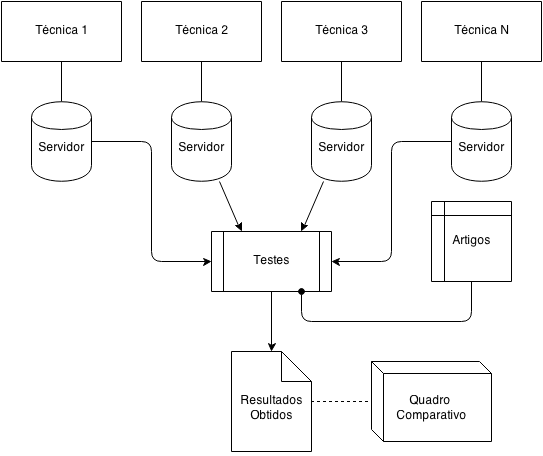
\includegraphics[width=0.8\linewidth]{./assets/images/metodology}
    \center\footnotesize{Fonte: O próprio autor}
\end{figure}


\section{Escolha do Corpus}
\label{sec:corpus}

% Falar da seleção de artigos de várias áreas

Visando provar a eficiência das ferramentas - juntamente com a implementação das técnicas por elas utilizadas -, desejamos ter resultados exatos da extração de metadados, de maneira que possam ser comparados e verificados com os metadados manualmente extraídos. Deste modo, foi selecionada uma série de artigos científicos das mais diversas áreas de pesquisa, com padrões visuais distintos.

% Porque selecionar artigos de diferentes áreas

Em virtude da necessidade de realizar testes com as ferramentas selecionadas em um ambiente real e representativo, foi realizada uma pesquisa no site do CNPq \url{http://www.cnpq.br/} a fim de obter a relação das áreas e subáreas do conhecimento reconhecidas oficialmente. Deste modo foi constatada a existência de 9 (nove) áreas do conhecimento, totalizando 1.288 (mil duzentas e oitenta e oito) subáreas, conforme pode ser verificado na \autoref{tab:areas-cnpq}.

\begin{table}
    \caption{Áreas do Conhecimento (CNPq)}
    \begin{center}
        \begin{tabular}{|l|c|}
            \hline 
            \textbf{Áreas do Conhecimento} & \textbf{Subáreas} \\ 
            \hline 
            Ciências Agrárias & 157 \\
            Ciências Biológicas & 104 \\
            Ciências da Saúde & 76 \\
            Ciências Exatas e da Terra & 243 \\
            Ciências Humanas & 163 \\
            Ciências Sociais Aplicadas & 185 \\
            Engenharias & 305 \\
            Lingüística, Letras e Artes & 53 \\
            Outros & 4 \\
            \hline
            \textbf{Total} & \textbf{1288} \\
            \hline
        \end{tabular}
    \end{center}
    \center\footnotesize{Fonte: \url{http://www.memoria.cnpq.br/areasconhecimento/index.htm}}
    \label{tab:areas-cnpq}
\end{table}

Com base no grande número de subdivisões de cada área do conhecimento (vide \autoref{tab:areas-cnpq}), a seleção das subáreas será limitada a 2 (duas), sendo a escolha feita com base na existência de curso de graduação e/ou departamento na Universidade Federal de Minas Gerais (UFMG), o que facilitaria o contato com professores e coordenadores dos respectivos cursos. Desta forma, excluindo-se a área ``Outros'', seriam analisadas 16 (dezesseis) subáreas, sendo 2 (duas) para cada uma das 8 (oito) áreas do conhecimento.

Com as subáreas selecionadas, foi realizada uma entrevista com professores e/ou coordenadores de cada curso ou departamento correspondente na UFMG, obtendo então as bases de dados e/ou revistas mais utilizadas e relevantes para cada subárea do conhecimento, construindo um \emph{corpus} realmente significativo. A relação dos professores entrevistados e as subáreas do conhecimento selecionadas pode ser vista na \autoref{tab:subareas-professores}.

\begin{table}
    \caption{Professores entrevistados para cada subárea do conhecimento.}
    \begin{center}
        \begin{tabular}{|p{6cm}|p{8cm}|}
            \hline 
            \textbf{Subárea do Conhecimento} & \textbf{Professor(a)}\\ 
            \hline 
            Arquitetura e Urbanismo & Eleonora Sad de Assis \\
            \hline
            Ciência da Computação & Adriano Alonso Veloso \par 
                                    Alberto Henrique Frade Laender \par 
                                    Arnaldo de Albuquerque Araújo \\
            \hline
            Ciência da Informação & Beatriz Valadares Cendón \\
            \hline
            Ciências Biológicas (Genética) & Mônica Bucciarelli Rodriguez \\
            \hline
            Ciências Biológicas (Zoologia) & Alfredo Hannemann Wieloch \\
            \hline
            Enfermagem & Eline Lima Borges \par
                         Tania Couto Machado Chianca \par
                         Daclé Vilma Carvalho \\
            \hline
            Engenharia Civil & Antônio Neves de Carvalho Júnior \\
            \hline
            Engenharia Mecânica & Antônio Eustáquio de Melo Pertence \par
                                  Alexandre Mendes Abrao \\
            \hline
            Fonoaudiologia & Sirley Alves da Silva Carvalho \\
            \hline
            Geologia & Adolf Heinrich Horn \\
            \hline
            História & Adriana Romeiro \\
            \hline
            Letras & Adriana Silvina Pagano \\
            \hline
            Medicina Veterinária & João Paulo Amaral Haddad \par
                                   Jenner Karlisson Pimenta dos Reis \\
            \hline
            Música & João Pedro Paiva de Oliveira \\
            \hline
            Psicologia & Carmen Elvira Flores-Mendoza Prado \par
                         Livia de Oliveira Borges \\
            \hline
            Zootecnia & Ângela Maria Quintão Lana \\
            \hline
        \end{tabular}
    \end{center}
    \label{tab:subareas-professores}
\end{table}

Para cada uma das subáreas do conhecimento selecionadas foram coletados 7 (sete) artigos científicos. Em virtude da diversidade de quantidade de bases de dados informadas pelos professores de cada subárea do conhecimento (\autoref{tab:databases}), a pesquisa foi limitada a 2 (duas) bases, na ordem apresentada pelos próprios pesquisadores, contemplando 4 (quatro) artigos para a primeira base e 3 (três) para a segunda. Para a subárea ``Ciências Biológicas (Genética)'' somente uma base de dados será utilizada, portanto dela serão retirados os 7 artigos necessários. No total foram selecionados 112 (cento e doze) artigos, contemplando 16 subáreas do conhecimento e 32 bases de dados, formando então o \emph{corpus} utilizado como base desta pesquisa.

\begin{table}
    \caption{Bases de Dados informadas pelos professores entrevistados, por subárea do conhecimento.}
    \begin{center}
        \begin{tabular}{|p{6cm}|p{8cm}|}
            \hline 
            \textbf{Subárea do Conhecimento} & \textbf{Bases de Dados} \\ 
            \hline 
            Arquitetura e Urbanismo & Scielo, Web of Science, Scopus \\
            \hline
            Ciência da Computação & DBLP, ACM Digital Library, IEEE Xplore \\
            \hline
            Ciência da Informação & LISA, ISTA, LISTA \\
            \hline
            Ciências Biológicas (Genética) & PubMed \\
            \hline
            Ciências Biológicas (Zoologia) & Zoological Records, Biological Abstracts \\
            \hline
            Enfermagem & MedLine, Lilacs, CINAHL, EBSCO, IBECS, BDENF \\
            \hline
            Engenharia Civil & Construction and Building Materials (ELSEVIER), Cement and Concrete Composites (ELSEVIER), Composites Science and Technology (ScienceDirect), Cement and Concrete Research (ELSEVIER), Materials Research (Scielo) \\
            \hline
            Engenharia Mecânica & Scopus, ScienceDirect, Web of Science, SpringerLink, Elsevier, Research Gate \\
            \hline
            Fonoaudiologia & Pubmed, Bireme \\
            \hline
            Geologia & Springer, Scielo, Portal CAPES \\
            \hline
            História & Scielo, Jstor, Redalyc \\
            \hline
            Letras & Delta (Scielo), Periódicos Letras UFMG, Periódicos UFSC \\
            \hline
            Medicina Veterinária & PubMed, Scielo \\
            \hline
            Música & RISM, RILM, JSTOR, Grove Dictionary of Music \\
            \hline
            Psicologia & Scopus, PsycInfo, Scopus, Psicodoc \\
            \hline
            Zootecnia & Dairy Science, Animal, Poutry Science \\
            \hline
        \end{tabular}
    \end{center}
    \label{tab:databases}
\end{table}

A seleção dos artigos em cada base de dados foi feita de maneira arbitrária, levando em consideração diferenças de leiautes e posicionamento dos elementos, permitindo que uma maior variedade de documentos seja analisada.

% Artigos em Inglês, somente

Todos os artigos selecionados foram escritos na língua inglesa. Esta decisão foi tomada em virtude de, além de ser a língua inglesa a universal para disseminação de conhecimento, ela é a mais utilizada no meio acadêmico, possuindo um universo muito maior e mais rico de artigos escritos no idioma. Além disso, algumas das ferramentas e respectivas técnicas utilizadas nos testes utilizam de ``processamento de linguagem natural'' para extração dos metadados, tendo por padrão a utilização do inglês na análise dos textos dos documentos.

Em virtude destas colocações a abrangência de outros idiomas entraria em um aspecto que não é objetivo deste trabalho abordar, visto a diversificação de culturas e símbolos, fazendo com que línguas orientais, como o mandarim ou japonês por exemplo, tenham análises diferenciadas em função de suas diferenças nas formas de representação e leitura, necessitando de outras técnicas e/ou ferramentas mais direcionadas a fim de obter os resultados esperados.

No que tange a escolha das ferramentas para testes foi utilizado apenas um ponto na seleção: a sua utilização por linha de comando (\emph{command line}). Embora algumas ferramentas possuem código aberto a extração de metadados faz parte de um contexto específico da aplicação, dificultando a utilização de apenas este recurso. Assim, foram selecionadas para testes apenas as ferramentas que permitem o uso de sua funcionalidade de extração de metadados de maneira individual, independente da linguagem de programação ou tecnologia apresentada. 

Deste modo, dentre as ferramentas apresentadas neste trabalho, presentes na \autoref{tab:tools-consolidated}, as ferramentas selecionadas para teste foram: Cermine, CiteSeer, CrossRef e ParsCit.
    

\section{Desenho do Experimento}
\label{sec:experiment-design}

Tendo selecionadas as ferramentas e os artigos que serão utilizados para os testes, parte-se para a instalação adequada de cada ferramenta, juntamente com as tecnologias necessárias e as linguagens de programação utilizadas pelos seus desenvolvedores. 

Cada ferramenta será testada em separado, observando suas características particulares. Assim, cada artigo selecionado será testado para aquela ferramenta, anotando os resultados obtidos na extração. Estes resultados serão separados por metadados, o que permitirá calcular qual a porcentagem de acerto que cada ferramenta teve na extração de cada metadado analisado.

Assim, o processo será repetido para cada ferramenta e o resultado registrado, permitindo calcular sua porcentagem total de acertos de maneira simplificada. Para isso será criado um ``Quadro Comparativo'', no qual serão inseridos os resultados dos testes de cada ferramenta. 

\subsection{Metadados, Pesos e Resultados}
\label{ssec:metadata-results}

% Importância de se ter pesos em função dos metadados

Em se tratando de pesquisa por artigos científicos, pequenos detalhes podem fazer a diferença. Desta forma, uma extração de metadados não muito eficaz pode prejudicar direta ou indiretamente os resultados apresentados por esta busca. Por outro lado, alguns metadados tendem a ser mais utilizados na pesquisa que outros, o que implica em uma responsabilidade maior na eficiência de sua extração. 

% Quais metadados são mais importantes para uma pesquisa de artigos

Geralmente quando vamos buscar artigos, procuramos primeiro pelo título (quando procuramos por um documento específico) ou então pelo nome do autor (quanto procuramos por artigos de um determinado pesquisador). Deste modo serão atribuídos pesos para cada um dos metadados, de maneira a valorizar a extração destas informações que podem influenciar diretamente os resultados de busca.

Deste modo apresentamos a \autoref{tab:metadata-weight}, que demonstra como cada metadado deve ser interpretado e qual o peso que lhe será atribuído, sendo utilizado o inteiro 1 (um) para o peso mais baixo e o 5 (cinco) para o peso mais alto, sendo consequentemente o(s) metadado(s) mais importante(s). Os pesos utilizados, assim como a ordem de importância escolhida foram fundamentados de maneira arbitrária, baseados na experiência do autor.

% Tabela de metadados e pesos

\begin{table}
    \caption{Os metadados e seus pesos atribuídos}
    \begin{center}
        \begin{tabular}{|p{3cm}|p{8cm}|C{1cm}|}
            \hline \textbf{Metadado} & \textbf{Relevância} & \textbf{Peso} \\ 
            \hline Título & Um dos termos mais buscados quando se pesquisa um artigo & 5 \\
            \hline Autor(es) & Outro termo muito utilizado na busca por artigos & 4 \\
            \hline E-mail(s) & Pouco relevante no quesito pesquisa de artigos & 1 \\
            \hline Resumo & Importante por conter palavras chaves e o resumo propriamente dito & 3 \\
            \hline Referências & Muito importante e necessário, pois será utilizada na referência inversa de autores & 4 \\
            \hline 
        \end{tabular} 
    \end{center}
    \label{tab:metadata-weight}
\end{table}

Como a extração de um metadado nem sempre ocorre de maneira 100\% eficaz, visando uma avaliação mais detalhada de cada ferramenta, será calculada a precisão do resultado da extração de cada metadado, feita com base na porcentagem de sucesso obtida para aquele conjunto de caracteres. Este cálculo será feito com o uso da função \texttt{similar\_text} da linguagem de programação PHP \url{http://php.net/similar_text}, que calcula a porcentagem de similaridade entre dois textos de acordo com o algoritmo proposto por Oliver \cite{oliver-1993}. Assim, serão comparados:

\begin{enumerate}
    \item O dado correto, retirado manualmente dos artigos;
    \item O dado extraído, obtido por cada ferramenta.
\end{enumerate}

Esta taxa de acerto será referenciada posteriormente, como por exemplo, por $P_{título}$ (porcentagem de acerto para o metadado título). Segundo a documentação da função \texttt{similar\_text} temos:

\begin{quote}
    \emph{``This calculates the similarity between two strings as described in Programming Classics: Implementing the World's Best Algorithms by Oliver (ISBN 0-131-00413-1). Note that this implementation does not use a stack as in Oliver's pseudo code, but recursive calls which may or may not speed up the whole process. Note also that the complexity of this algorithm is O(N**3) where N is the length of the longest string.''}
\end{quote}

Esta função recebe três parâmetros: o primeiro texto, o segundo texto e uma variável onde será armazenada a porcentagem de acerto. Como retorno é retornado um inteiro representando o número de caracteres em comum entre os dois textos comparados. Sua estrutura de utilização é a seguinte:

\lstset{language=PHP}
\begin{lstlisting}[escapechar=\#]
int similar_text ( string $first , string $second [, float &$percent ] )
\end{lstlisting}

Como cada ferramenta será testada em separado, os resultados da extração de cada artigo serão registrados, tendo o total da precisão calculado de acordo com a média aritmética dos resultados obtidos para aquele metadado. Por exemplo, para a Ferramenta ``A'' serão analisados 100 (cem) artigos. A precisão na extração do título de cada artigo ($P_{título1}$, $P_{título2}$, ..., $P_{títuloN}$), por exemplo, será somada e o resultado dividido pelo número de artigos - no caso 100. Assim tem-se a precisão geral para o metadado ``Título'' da Ferramenta ``A'' ($P_{título}$):

\begin{center}
    \begin{math}
        P_{título} = (P_{título1} + P_{título2} + P_{título3} ... + P_{título100}) / 100
        \label{math:result-by-metadata}
    \end{math}
\end{center}

De posse dos resultados para cada metadado extraído podemos comparar as ferramentas a fim de obter qual é mais adequada para cada tipo de metadado. Podemos inferir, portanto, que a ferramenta ``X'' apresenta melhores resultados do que ``Y'' na extração do nome dos autores, por exemplo.

\subsection{Índice de Confiabilidade}
\label{ssec:confiability-index}

% Fórmula final para a nota final de cada técnica

Considerando que cada metadado possui um peso diferente necessitamos calcular o índice de acertos a ser utilizado em cada resultado coletado para cada ferramenta testada. Assim chegamos a uma fórmula matemática à qual chamaremos ``Índice de Confiabilidade'', que calcula o resultado obtido através dos pesos que foram atribuídos a cada metadado, para cada ferramenta. Este índice é a nota final de cada ferramenta, levando em consideração todos os resultados obtidos por ela para o conjunto de artigos testado neste trabalho.

Este índice utiliza os pesos anteriormente definidos e a precisão dos resultados obtida, de maneira a permitir chegar a uma única nota final para cada ferramenta testada.

Esta fórmula é a média ponderada dos resultados alcançados na extração de cada metadado dos artigos, seguindo os pesos apresentados na \autoref{tab:metadata-weight}. Cada peso é atribuído ao resultado encontrado em cada ferramenta. 

A título de exemplo, após o teste de uma ferramenta, supondo que ela conseguiu extrair 87\% dos títulos de todos artigos com sucesso, sua precisão com relação ao título será 87 ($P_{título}=87$), que será multiplicada pelo peso correspondente, neste caso, o inteiro 5. Isso ocorre para todos os metadados extraídos, seguindo seus respectivos pesos. A descrição de cada variável no Índice de Confiabilidade poderá ser obtida de acordo com a \autoref{tab:confiability-index}.

\begin{center}
    $ IC_{Ferramenta X}=(5*P_{título}+4*P_{autor}+1*P_{email}+3*P_{resumo}+4*P_{referências}) / 17 $
\end{center}

\begin{table}
    \caption{Descrição de cada variável no Índice de Confiabilidade}
    \begin{center}
        \begin{tabular}{|p{3cm}|p{8cm}|}
            \hline \textbf{Variável} & \textbf{Descrição}\\ 
            \hline $P_{título}$ & Precisão na obtenção do título \\
            \hline $P_{autor}$ & Precisão na obtenção do(s) autor(es)\\
            \hline $P_{email}$ & Precisão na obtenção dos e-mails dos autores \\
            \hline $P_{resumo}$ & Precisão na obtenção do resumo \\
            \hline $P_{referências}$ & Precisão na obtenção das referências \\
            \hline 
        \end{tabular} 
    \end{center}
    \label{tab:confiability-index}
\end{table}

Assim, de posse do Índice de Confiabilidade de cada ferramenta podemos classificar cada uma com base nos seus resultados apresentados. Esta classificação será feita de maneira arbitrária, sem objetivo algum de denegrir alguma ferramenta em favorecimento de outra, mas sim classificar cada uma delas com base nos resultados obtidos e critérios adotados neste trabalho. Desta forma, podemos classificar cada ferramenta seguindo os tópicos abaixo:

\begin{enumerate}
    \item \textbf{Precisa (P):} Quando o Índice de Confiabilidade é maior ou igual a 80 ($IC\geq80$).
    \item \textbf{Satisfatória (S):} Quando o Índice de Confiabilidade é maior ou igual a 60 e menor que 80 ($60 \leq IC < 80$).
    \item \textbf{Insatisfatória (I):} Quando o Índice de Confiabilidade é menor que 60 ($IC < 60$).
\end{enumerate}

\section{Ambiente Tecnológico}
\label{sec:tech-environment}

As ferramentas testadas, por utilizarem das mesmas linguagens de programação ou por terem seu conjunto tecnológico muito semelhante, serão instaladas em um único servidor, permitindo que recursos computacionais sejam compartilhados, simplificando o trabalho de configuração em função de suas necessidades parecidas.

Este servidor será criado através de máquina virtual, o que traz benefícios não somente de performance mas de flexibilidade quanto das tecnologias necessárias para o funcionamento de cada ferramenta, permitindo que os testes possam ser feitos em sistemas operacionais distintos mas utilizando dos mesmos recursos computacionais da máquina de origem.




% Análise e Apresentação de Resultados
%!TEX root = ../masters.tex

\chapter{Análise e Apresentação de Resultados}
\label{cha:results}

% Construção da teoria

% Falar sobre o corpus e as ferramentas (FEITO)

Com o Corpus totalmente definido e as ferramentas devidamente instaladas no ambiente de testes foram realizados diversos experimentos para que os resultados pudessem ser analisados e comparados numericamente.

% Falar das dificuldades encontradas na extração (FEITO)

Durante a extração dos metadados algumas observações puderam ser feitas tanto pela análise manual de cada resultado individual como também dos resultados em conjunto, tendo em vista os números apresentados pelas ferramentas utilizadas.

A ferramenta Cermine demonstrou-se de bem simples execução. Por se tratar de um arquivo em formato \texttt{.jar} (Java) em forma executável, a extração ocorreu de maneira fluida, com os dados de saída da ferramenta gravados em arquivos isolados para posterior comparação. Além disso, os resultados apresentados foram os mais completos, com utilização de diversas \emph{tags} XML que permitiram uma fácil manipulação dos dados, com uma grande riqueza de detalhes. O processo de extração dos metadados para a ferramenta Cermine foi o mais lento das 4 (quatro) ferramentas testadas, demorando entre 15 (quinze) e 20 (vinte) segundos para uma completa análise de cada artigo.

Já a ferramenta CiteSeer foi a que mais exigiu conhecimentos técnicos para que pudesse ser testada. Sua execução dependeu da instalação de diversos outros componentes e serviços de terceiros, o que contribuiu para um aumento da complexidade de seu uso. Um fato interessante é que a ferramenta utiliza de outras ferramentas para alguns processos específicos de extração, como é o caso da sessão de referências, onde utiliza a ferramenta ParsCit. Embora a ferramenta utilizada seja a mesma a forma de entrada de dados é diferenciada, implicando em resultados numericamente diferentes.

No caso da ferramenta CrossRef algumas particularidades devem ser mencionadas. Seus resultados de extração são apresentados de maneira muito básica, com campos muito genéricos e resultados pouco precisos, dificultando um pós-processamento dos dados. Os metadados ``autores'', ``e-mails'' e ``resumo'' não puderam ser extraídos. A versão atual de desenvolvimento da ferramenta não permite uma separação de dados muito específica, agrupando diversas informações em tags chamadas ``sections''. Estas tags possuem informações textuais gerais, não sendo possível serem filtradas com a utilização da própria ferramenta. Portanto, para a ferramenta CrossRef somente os metadados ``título'' e ``referências'' foram extraídos e considerados. Os resultados para a extração das referências também merecem considerações, por serem apresentados de maneira muito genérica, em uma única tag XML, sendo impossível separar título e autor dentro do conteúdo retornado.

A ferramenta ParsCit também foi utilizada sem maiores dificuldades. Em virtude de sua particularidade de processar apenas dados de entrada em formato texto ou XML, conforme sugerido pelos desenvolvedores, foi utilizada a ferramenta de linha de comando \texttt{pdftotext} (disponível em ambiente Linux) para conversão dos artigos em \texttt{.pdf} em arquivos \texttt{.txt}, permitindo que a ferramenta fosse utilizada conforme recomendações. Esta conversão foi feita em tempo de execução e os resultados coletados e gravados com sucesso.

De modo geral, exceto pela ferramenta CrossRef as demais ferramentas tiveram um processo de extração bem eficaz visualmente e dentro do esperado, em virtude da grande diferenciação visual testada com o Corpus selecionado. 

% Falar das particularidades nos algoritmos de comparação (FEITO)

No que diz respeito à comparação dos resultados foi necessária uma padronização dos dados para que as quatro ferramentas pudessem ser testadas de maneira uniforme. Em virtude de apresentar resultados bastante detalhados, a ferramenta Cermine permitiu que os autores das referências fossem retornados seguindo a forma ``primeiro nome'' e em seguida ``sobrenome''. Já as demais ferramentas não apresentaram os resultados com tanta flexibilidade, variando em alguns momentos a ordem e disposição do nome dos autores. Assim, foi necessário um pré-processamento computacional a fim de manter, quando possível, o primeiro nome antes do sobrenome, tornando as comparações mais padronizadas e justas. Este pré-processamento foi realizado para todas as ferramentas testadas.

Já para a extração do metadado ``e-mails'', algumas ferramentas extraíram mais informações em conjunto, como foi o caso de algumas poucas extrações realizadas pela ferramenta Cermine. Em um destes casos a ferramenta retornou como e-mail o seguinte conteúdo: \texttt{Email: mvpein@yahoo.com}. Assim, sempre visando uma justa comparação entre as ferramentas foi realizada uma análise em todos os resultados deste metadado para que somente pudessem ser comparados endereços de e-mails, o que tornou o processo bem simplificado e correto. Os endereços de e-mail foram filtrados com a utilização de expressão regular (\autoref{sssec:regular-expressions}) alcançando um conjunto homogêneo de dados comparados.

Os demais metadados foram comparados sem problemas. O metadado ``título'' foi utilizado sem sua pontuação final, retirando antes da comparação qualquer caractere passível de erros como: asteriscos, pontos finais e espaços em branco. O resultado das extrações dos título foi feito seguindo a lógica anteriormente apresentada, comparando a similaridade entre os dois textos através do uso da função \texttt{similar\_text} da linguagem de programação PHP, que apresenta como resultado um valor numérico representando o percentual de similaridade. Esta mesma lógica descrita foi aplicada para o metadado ``resumo''.

Os nomes dos autores foram comparados seguindo a mesma lógica do metadado ``título'', porém levando em consideração a ordem de apresentação e extração dos mesmos. Sendo assim, além de verificar a similaridade entre os nomes os testes levaram em consideração a ordem de apresentação dos resultados de cada ferramenta.

% Falar também da questão dos nomes dos autores com acentos, no caso de autores russos, croatas e latinos. Algumas ferramentas retornaram os resultados sem acento o que implica em uma comparação menos precisa. (FEITO)

Dentro do Corpus escolhido diversos nomes de autores continham acentos e caracteres característicos de seu idioma de origem, como é o caso da autora polonesa ``Anna Białk-Bielińska''. Em virtude desta questão, as ferramentas se comportaram de maneiras distintas. Algumas conseguiram extrair os nomes como no artigo original, porém, outras substituíram caracteres como ``ń'' por apenas ``n'', ou ainda ``n´''. Algumas ferramentas simplesmente desprezaram estes caracteres.

No caso específico do metadado ``e-mail'' a comparação foi realizada com base na identificação correta ou não do endereço eletrônico. Neste caso não foi considerada a porcentagem de similaridade entre resultados, ou seja, o endereço foi corretamente identificado ou não. Para estes resultados foram utilizados os inteiros 0 (zero) para a extração ineficiente e 100 (cem) para a extração eficiente.

% Falar que considerei apenas os artigos que possuem email. Os que não tinha o cálculo da média desconsidera os resultados, marcando-os como -1. (FEITO)

Uma grande parte dos artigos utilizados no Corpus deste trabalho não continha informações de e-mail dos autores. Desta forma, as extrações destes documentos foram desconsideradas, permitindo que as ferramentas tivessem seus resultados avaliados apenas para as extrações realmente computadas, valorizando ainda mais o trabalho de cada uma.

% Sobre a comparação dos Títulos (FEITO)

Já para a comparação das referências foram utilizadas duas informações: o título e o nome dos autores. Para o caso do título das referências, a lógica utilizada foi a mesma para o metadado ``título'', utilizando-se de um valor percentual representando a similaridade entre os dados comparados. Já para o nome dos autores, a lógica seguiu a mesma do metadado ``autores'', onde foram consideradas tanto a similaridade textual como também a ordem de apresentação. Deste modo, a extração de cada referência considerou um peso de 60\% do resultado para o título e 40\% para os nomes dos autores, chegando em um numero final que representasse o resultado da extração de cada referência comparada.

% Resultados das comparações (FEITO)

Com os dados de cada extração armazenados a comparação foi feita de maneira automática levando em consideração todos os pontos apresentados acima. Para cada subárea do conhecimento foi realizada uma comparação, registrando o resultado consolidado para cada artigo extraído, bem como a média aritmética dos resultados daquela subárea em específico. Portanto, para cada ferramenta e subárea, foi registrado um valor médio dos resultados.

Posteriormente foi feita a coleta destes dados separados por subáreas, porém consolidando-os para cada ferramenta. Assim, foi calculada a média aritmética dos resultados de cada ferramenta para todas as subáreas analisadas, chegando então a uma nota final em cada metadado extraído, possibilitando então o cálculo do ``Índice de Confiabilidade'' (\autoref{ssec:confiability-index}) para cada ferramenta.

% Trabalhar as evidências de que sua hipótese é verdadeira

\section{Resultados}
\label{sec:results}

% Apresentar dados, testes, provas, estudos de caso, etc

Conforme esperado os resultados foram coletados de maneira individualizada - para cada artigo - e consolidados de maneira geral para cada ferramenta e metadado. Os resultados apresentados por área do conhecimento estão presentes em 4 (quatro) tabelas, separadas por cada uma das ferramentas. 

Os resultados da ferramenta Cermine estão presentes na \autoref{tab:results-cermine}. Os resultados da CiteSeer estão na \autoref{tab:results-citeseer}. Os resultado da ferramenta CrossRef na \autoref{tab:results-crossref} e da ParsCit na \autoref{tab:results-parscit}. Todas as tabelas mostram o percentual de acerto separados por subárea do conhecimento e por metadados, representados pelas colunas Tit. (Título),  Aut. (Autores), Ema. (E-mails), Res. (Resumo) e Ref. (Referências).

\begin{table}
    \caption{Resultados da ferramenta Cermine por subárea do conhecimento.}
    \begin{center}
        \begin{tabular}{|p{6cm}|C{1.2cm}|C{1.2cm}|C{1.2cm}|C{1.2cm}|C{1.2cm}|}
            \hline 
            \textbf{Subárea do Conhecimento} & \textbf{Tit.} & \textbf{Aut.} & \textbf{Ema.} & \textbf{Res.} & \textbf{Ref.} \\ \hline 
            Arquitetura e Urbanismo & 100 & 58.75 & 16.67 & 99.01 & 82.67 \\ \hline
Ciência da Computação & 88.27 & 71.87 & 21.43 & 98.83 & 77.25 \\ \hline
Ciência da Informação & 76.55 & 61.90 & 28.57 & 78.02 & 53.81 \\ \hline
Ciências Biológicas (Genética) & 91.58 & 81.00 & 50.00 & 84.72 & 96.11 \\ \hline
Ciências Biológicas (Zoologia) & 99.78 & 73.16 & 42.86 & 84.74 & 72.28 \\ \hline
Enfermagem & 99.77 & 39.38 & 16.67 & 98.09 & 81.69 \\ \hline
Engenharia Civil & 71.43 & 76.34 & 37.50 & 94.18 & 56.23 \\ \hline
Engenharia Mecânica & 99.45 & 75.97 & 58.33 & 77.97 & 82.87 \\ \hline
Fonoaudiologia & 100 & 77.75 & 71.43 & 98.13 & 80.05 \\ \hline
Geologia & 99.54 & 100 & 66.67 & 53.66 & 64.03 \\ \hline
História & 99.20 & 89.29 & 50.00 & 65.59 & 53.40 \\ \hline
Letras & 88.01 & 99.50 & 42.86 & 82.10 & 86.74 \\ \hline
Medicina Veterinária & 85.71 & 91.11 & 85.71 & 98.77 & 80.05 \\ \hline
Música & 99.03 & 90.61 & 66.67 & 95.47 & 68.50 \\ \hline
Psicologia & 88.46 & 63.96 & 47.62 & 92.53 & 63.25 \\ \hline
Zootecnia & 49.95 & 70.82 & 42.86 & 87.40 & 81.99 \\ \hline
\textbf{Média Geral} & 89.80 & 76.34 & 46.62 & 86.83 & 73.81 \\ \hline

        \end{tabular}
    \end{center}
    \label{tab:results-cermine}
\end{table}

\begin{table}
    \caption{Resultados da ferramenta CiteSeer por subárea do conhecimento.}
    \begin{center}
        \begin{tabular}{|p{6cm}|C{1.2cm}|C{1.2cm}|C{1.2cm}|C{1.2cm}|C{1.2cm}|}
            \hline 
            \textbf{Subárea do Conhecimento} & \textbf{Tit.} & \textbf{Aut.} & \textbf{Ema.} & \textbf{Res.} & \textbf{Ref.} \\ \hline 
            Arquitetura e Urbanismo & 100 & 96.89 & 0 & 97.43 & 70.95 \\ \hline
Ciência da Computação & 100 & 83.75 & 23.81 & 99.81 & 71.79 \\ \hline
Ciência da Informação & 84.44 & 99.50 & 0 & 74.12 & 55.56 \\ \hline
Ciências Biológicas (Genética) & 80.92 & 83.15 & 28.57 & 60.63 & 25.15 \\ \hline
Ciências Biológicas (Zoologia) & 57.14 & 64.12 & 0 & 71.14 & 70.10 \\ \hline
Enfermagem & 71.43 & 52.82 & 0 & 70.31 & 34.67 \\ \hline
Engenharia Civil & 97.81 & 62.42 & 0 & 71.18 & 35.61 \\ \hline
Engenharia Mecânica & 71.11 & 46.00 & 0 & 71.36 & 63.18 \\ \hline
Fonoaudiologia & 100 & 61.14 & 0 & 94.68 & 61.85 \\ \hline
Geologia & 73.77 & 34.69 & 0 & 42.79 & 57.13 \\ \hline
História & 99.53 & 71.09 & 0 & 65.26 & 63.81 \\ \hline
Letras & 99.57 & 85.73 & 0 & 75.78 & 58.82 \\ \hline
Medicina Veterinária & 85.71 & 86.38 & 0 & 98.88 & 63.53 \\ \hline
Música & 49.02 & 56.87 & 0 & 54.28 & 54.55 \\ \hline
Psicologia & 94.93 & 83.85 & 14.29 & 88.87 & 66.75 \\ \hline
Zootecnia & 71.43 & 82.41 & 0 & 76.39 & 22.59 \\ \hline
\textbf{Média Geral} & 83.55 & 71.93 & 4.17 & 75.81 & 54.75 \\ \hline

        \end{tabular}
    \end{center}
    \label{tab:results-citeseer}
\end{table}

\begin{table}
    \caption{Resultados da ferramenta CrossRef por subárea do conhecimento.}
    \begin{center}
        \begin{tabular}{|p{6cm}|C{1.2cm}|C{1.2cm}|C{1.2cm}|C{1.2cm}|C{1.2cm}|}
            \hline 
            \textbf{Subárea do Conhecimento} & \textbf{Tit.} & \textbf{Aut.} & \textbf{Ema.} & \textbf{Res.} & \textbf{Ref.} \\ \hline 
            Arquitetura e Urbanismo & 72.68 & 0 & 0 & 0 & 22.79 \\ \hline
Ciência da Computação & 64.19 & 0 & 0 & 0 & 14.64 \\ \hline
Ciência da Informação & 32.32 & 0 & 0 & 0 & 8.14 \\ \hline
Ciências Biológicas (Genética) & 47.05 & 0 & 0 & 0 & 14.62 \\ \hline
Ciências Biológicas (Zoologia) & 70.70 & 0 & 0 & 0 & 32.72 \\ \hline
Enfermagem & 55.96 & 0 & 0 & 0 & 10.29 \\ \hline
Engenharia Civil & 74.70 & 0 & 0 & 0 & 12.21 \\ \hline
Engenharia Mecânica & 89.27 & 0 & 0 & 0 & 27.50 \\ \hline
Fonoaudiologia & 71.43 & 0 & 0 & 0 & 13.92 \\ \hline
Geologia & 97.62 & 0 & 0 & 0 & 15.72 \\ \hline
História & 64.08 & 0 & 0 & 0 & 16.11 \\ \hline
Letras & 75.66 & 0 & 0 & 0 & 32.58 \\ \hline
Medicina Veterinária & 49.66 & 0 & 0 & 0 & 23.09 \\ \hline
Música & 84.63 & 0 & 0 & 0 & 28.16 \\ \hline
Psicologia & 82.92 & 0 & 0 & 0 & 23.19 \\ \hline
Zootecnia & 32.05 & 0 & 0 & 0 & 25.21 \\ \hline
\textbf{Média Geral} & 66.56 & 0 & 0 & 0 & 20.06 \\ \hline

        \end{tabular}
    \end{center}
    \label{tab:results-crossref}
\end{table}

\begin{table}
    \caption{Resultados da ferramenta ParsCit por subárea do conhecimento.}
    \begin{center}
        \begin{tabular}{|p{6cm}|C{1.2cm}|C{1.2cm}|C{1.2cm}|C{1.2cm}|C{1.2cm}|}
            \hline 
            \textbf{Subárea do Conhecimento} & \textbf{Tit.} & \textbf{Aut.} & \textbf{Ema.} & \textbf{Res.} & \textbf{Ref.} \\ \hline 
            Arquitetura e Urbanismo & 0 & 17.14 & 0 & 73.23 & 51.62 \\ \hline
Ciência da Computação & 37.54 & 58.36 & 47.62 & 74.82 & 69.72 \\ \hline
Ciência da Informação & 32.30 & 31.51 & 28.57 & 59.60 & 50.09 \\ \hline
Ciências Biológicas (Genética) & 8.97 & 1.17 & 0 & 40.91 & 39.76 \\ \hline
Ciências Biológicas (Zoologia) & 0 & 0 & 0 & 69.98 & 54.61 \\ \hline
Enfermagem & 11.06 & 14.29 & 0 & 65.65 & 37.24 \\ \hline
Engenharia Civil & 11.48 & 15.64 & 37.50 & 56.61 & 37.97 \\ \hline
Engenharia Mecânica & 14.29 & 23.23 & 22.22 & 55.93 & 55.34 \\ \hline
Fonoaudiologia & 5.70 & 0.89 & 0 & 27.74 & 62.52 \\ \hline
Geologia & 14.29 & 14.29 & 16.67 & 68.42 & 55.15 \\ \hline
História & 5.62 & 14.29 & 0 & 59.33 & 60.17 \\ \hline
Letras & 24.42 & 42.21 & 21.43 & 68.53 & 54.00 \\ \hline
Medicina Veterinária & 14.29 & 13.82 & 14.29 & 36.57 & 53.31 \\ \hline
Música & 34.24 & 42.86 & 0 & 81.39 & 55.73 \\ \hline
Psicologia & 14.29 & 14.29 & 14.29 & 71.14 & 68.84 \\ \hline
Zootecnia & 14.29 & 5.88 & 0 & 78.60 & 51.21 \\ \hline
\hline \textbf{Média Geral} & 15.17 & 19.37 & 12.66 & 61.78 & 53.58 \\ \hline

        \end{tabular}
    \end{center}
    \label{tab:results-parscit}
\end{table}

% Conceitos criados pelo autor (FEITO)

Para que os resultados pudessem ser melhores interpretados foi calculado o ``Índice de Confiabilidade'' de cada ferramenta, detalhado no capítulo de Metodologia (\autoref{ssec:confiability-index}). Para calcular este índice foram utilizadas as médias dos resultados de extração de todas as subáreas, com os devidos pesos para cada metadado, obtendo-se então uma nota geral para cada ferramenta. Os resultados calculados para este índice estão presentes na \autoref{tab:conf-index-results}.

\begin{table}
    \caption{Índice de Confiabilidade de cada ferramenta}
    \begin{center}
        \begin{tabular}{|p{3cm}|C{3cm}|}
            \hline 
            \textbf{Ferramenta} & \textbf{Resultado} \\ \hline 
            Cermine & 79.81 \\ \hline 
CiteSeer & 68.00 \\ \hline 
CrossRef & 24.30 \\ \hline 
ParsCit & 33.27 \\ \hline 

        \end{tabular}
    \end{center}
    \label{tab:conf-index-results}
\end{table}

De posse do ``Índice de Confiabilidade'' de cada ferramenta, conforme previsto na \autoref{ssec:confiability-index}, cada uma foi classificada de acordo com seus resultados de extração. Estes resultados e suas respectivas classificações estão presentes na \autoref{tab:tool-classification}.

\begin{table}
    \caption{Classificação de cada ferramenta.}
    \begin{center}
        \begin{tabular}{|p{3cm}|C{5.5cm}|p{4cm}|}
            \hline 
            \textbf{Ferramenta} & \textbf{Índice de Confiabilidade} & \textbf{Classificação} \\ \hline 
            Cermine & 79.81 & Satisfatória \\ \hline 
CiteSeer & 68.00 & Satisfatória \\ \hline 
CrossRef & 24.30 & Insatisfatória \\ \hline 
ParsCit & 33.27 & Insatisfatória \\ \hline 

        \end{tabular}
    \end{center}
    \label{tab:tool-classification}
\end{table}

\section{Ambiente de Testes}

Para a realização das extrações e das comparações foi criado um ambiente de testes contendo todas as tecnologias necessárias para que as ferramentas pudessem ser executadas dentro do esperado. Desta maneira, foi utilizado um servidor virtual com a seguinte configuração:

\begin{itemize}
    \item Sistema Operacional Linux Ubuntu 14.04 64 Bits
    \item 2GB de Memória RAM
    \item 20GB de Espaço em Disco
\end{itemize}

As tecnologias utilizadas foram instaladas de acordo com as recomendações de cada ferramenta, com suas dependências e necessidades de cada linguagem de programação. Foram instaladas as seguintes linguagens/bibliotecas, separadas de acordo com cada ferramenta:

\begin{itemize}
    \item \textbf{Cermine:} Java OpenJDK Runtime Environment 1.7.0\_79
    \item \textbf{CiteSeer:} Python 2.7.6, GROBID \url{https://github.com/kermitt2/grobid}, PDFBox \url{http://pdfbox.apache.org/}, PDF Classifier Jar, Java SE Environment (Maven). 
    \item \textbf{CrossRef:} Ruby 2.1.2p95, RubyGem \texttt{pdf-extract} 0.0.1 e \texttt{pdf-reader} 1.3.2.
    \item \textbf{ParsCit:} Perl 5.18.2, G++ Compiler e CRF++ 0.51. Diversas outras dependências da linguagem Perl foram também instaladas: Class::Struct, Getopt::Long, Getopt::Std, File::Basename, File::Spec, FindBin, HTML::Entities, IO::File, POSIX, XML::Parser, XML::Twig, XML::Writer e XML::Writer::String.
\end{itemize}



% Conclusao
%!TEX root = ../masters.tex

\chapter{Discussão / Trabalhos Futuros} % (fold)
\label{cha:conclusion}

Após todo o processo de pesquisa, de extração dos metadados pelas ferramentas analisadas e coleta de seus respectivos resultados, algumas considerações podem ser feitas, objetivando cumprir com os objetivos propostos no início do trabalho.

Os resultados apresentados, de modo geral, foram inferiores às expectativas do próprio autor, uma vez que as extrações não foram tão precisas quanto se imaginava. A grande diferença no layout dos elementos, presente no Corpus escolhido, realmente teve alto impacto nos resultados, principalmente no que diz respeito à extração dos autores e das referências.

De modo geral, as ferramentas Cermine e CiteSeer obtiveram resultados para a extração do metadado ``título'' bem positivos, atingindo entre 83 e 89\% de precisão. Já a ferramenta CrossRef ficou bem abaixo do esperado, com 66.56\% de precisão apenas, porém acima da última colocada, a ferramenta ParsCit, que conseguiu extrair com sucesso apenas 15.17\% dos resultados dos ``títulos'', muito abaixo do esperado.

Para o metadado ``autores'' a ferramenta com maior precisão foi a Cermine, que atingiu 76.34\%, resultado próximo da segunda colocada, a CiteSeer, com 71.93\%. Já as demais ferramentas não obtiveram êxito na extração dos nomes dos autores, ficando abaixo dos 20\% de acerto.

Para a extração dos e-mails dos autores o resultado obtido, de modo geral, foi relativamente pior. A ferramenta que obteve maior êxito na extração deste metadado foi a Cermine, que conseguiu obter apenas 46.62\% de sucesso. Os resultados para este metadado obtidos pela ferramenta CiteSeer foram bem inferiores às expectativas, pois somente 4.17\% dos endereços foram extraídos com sucesso, resultado inferior ainda à ferramenta ParsCit, que extraiu 12.16\%. Como informado no capítulo ``Resultados'' (\autoref{cha:results}) a ferramenta CrossRef não conseguiu realizar a extração de nomes de autores, endereços de e-mails e do resumo, sendo estes resultados desconsiderados nesta sessão.

Em virtude da grande variação de layout do Corpus, inclusive pela ausência de uma padronização para apresentação do metadado ``resumo'' \emph{abstract}, os resultados obtidos para este metadado superaram as expectativas do autor, visto que, exceto pela ferramenta CrossRef, todas as demais obtiveram resultados acima de 60\%, chegando a 86.83\% da ferramenta Cermine, maior precisão dentre as ferramentas. Estes resultados, embora ainda abaixo do considerado ``ideal'' foram positivos, principalmente em virtude de alguns artigos apresentarem este metadado de maneira bem diferente, com posicionamento bem divergente do habitual e, inclusive, sem indícios de que ali se apresentava o resumo do artigo.

Outro ponto onde as expectativas do autor não foram atingidas foi na extração das ``referências''. A ferramenta Cermine, mais uma vez, demonstrou-se mais precisa, conquistando 73.81\% de sucesso. A ferramenta CiteSeer, que utiliza da ParsCit para extração das referências, ao ser comparada com a própria ParsCit, produziu resultados ou pouco superiores, 54.75\% e 53.58\%, respectivamente. A diferença nos resultados se deve pelo fato da ferramenta ParsCit necessitar de arquivos \texttt{.txt} como entrada de dados. No caso das extrações realizadas pela própria ferramenta, os arquivos \texttt{.txt} foram gerados pelo programa \texttt{pdftotext}, conforme detalhado no capítulo de ``Resultados'' (\autoref{cha:results}), diferentemente da ferramenta CiteSeer, que transforma o arquivo \texttt{.pdf} em \texttt{.txt} de sua própria maneira, causando então uma pequena divergência nos resultados gerais (1.17\%). 

Já a ferramenta CrossRef obteve apenas 20.06\% de precisão na extração das referências, o que era esperado em função de sua extração com poucos detalhes, com apenas um único campo com todas as informações de cada referência. Embora os resultados da extração não tenham sido positivos, um detalhe interessante que merece uma atenção é a forma como esta ferramenta trata as referências. A ferramenta permite que elas sejam comparadas com o banco de dados existente no \url{http://api.crossref.org}, permitindo identificar exatamente quais artigos já foram catalogadas pelo site, gerando um grande controle sobre o conteúdo, inclusive relacionando-o. Para os artigos encontrados na base de dados do CrossRef é possível obter, inclusive, a descrição de cada um em formato BibTeX, com todas as informações relevantes para uma correta citação científica. Para este trabalho, em virtude dos poucos resultados obtidos, esta funcionalidade não foi utilizada na extração e na comparação.

Em se tratando da separação dos resultados por área do conhecimento as ferramentas Cermine e CiteSeer obtiveram destaque, conseguindo 100\% de acertos em 3 subáreas do conhecimento, porém para metadados diferentes. A ferramenta Cermine acertou todos os títulos das áreas de Arquitetura e Urbanismo e Fonoaudiologia, além de 100\% dos nomes dos autores da área de Geologia. Já a ferramenta CiteSeer conseguiu precisão total na extração dos títulos de Arquitetura e Urbanismo, Ciência da Computação e Fonoaudiologia. Já a ferramenta CrossRef obteve melhor resultado na extração dos títulos dos artigos da área de Geologia, obtendo 97.62\% de precisão, superando a ferramenta CiteSeer e ParsCit, que obtiveram 73.77\% e 14.29\% respectivamente.

Para a extração dos títulos dos artigos, os piores resultados foram encontrados nas áreas de Música (CiteSeer, com 49.02\%), Zootecnia (Cermine, com 49.95\% e CrossRef, com 32.05\%) e as áreas Ciências Biológicas (Zoologia) e Arquitetura e Urbanismo (ParsCit, com nenhum acerto).

A ferramenta Cermine se destacou na extração de títulos de 8 (oito) subáreas do conhecimento - Arquitetura e Urbanismo, Ciências Biológicas (Zoologia), Enfermagem, Engenharia Mecânica, Fonoaudiologia, Geologia, História e Música -, obtendo resultados superiores a 99\%, o que é considerado excelente. 

Para os autores, seus maiores destaques foram nas áreas de Geologia, Letras, Medicina Veterinária e Música, com resultados acima de 90\%. Na extração dos e-mails dos autores a ferramenta Cermine obteve resultados superiores a 85\% somente na área de Medicina Veterinária, seu melhor resultado para este metadado. Além disso, a ferramenta se destacou na extração dos resumos em 5 (cinco) áreas, com resultados acima dos 98\%, e na extração das referências de Ciências Biológicas (Genética), onde obteve resultados acima de 96\% de precisão.

Já a ferramenta CiteSeer demonstrou bem eficiente na extração dos títulos de 5 (cinco) subáreas: Arquitetura e Urbanismo, Ciência da Computação, Fonoaudiologia, História e Letras, com resultados superiores a 99\%. Para a extração dos nomes dos autores o resultado foi relevante em apenas 2 (duas) subáreas: Arquitetura e Urbanismo e Ciência da Informação, com precisão acima de 90\%. Já para os e-mails dos autores os resultados deixaram a desejar para 13 (treze) das 16 (dezesseis) subáreas, com 0\% de acerto, tendo resultados positivos apenas para as subáreas de Ciência da Computação, Ciências Biológicas (Genética) e Psicologia, porém com resultados abaixo dos 29\% de acerto.

Para a extração dos resumos dos artigos a ferramenta CiteSeer também se demonstrou bem eficiente, com resultados acima dos 90\% para 4 (quatro) subáreas: Arquitetura e Urbanismo, Ciência da Computação, Fonoaudiologia e Medicina Veterinária. Para as referências (onde o CiteSeer utiliza do ParsCit) os resultados deixaram a desejar, com resultados abaixo dos 72\%.

A ferramenta CrossRef se demonstrou positiva apenas para a extração de títulos de artigos da subárea de Geologia, como já dito anteriormente, com 97.62\% de acerto, não tendo resultados considerados satisfatórios para as demais áreas. Já para a extração das referências os resultados também deixaram a desejar, com apenas 2 (duas) subáreas com precisão próxima de 30\%: Ciências Biológicas (Zoologia), com 32.72\% e Letras, com 32.58\%.

Por fim, a ferramenta ParsCit obteve resultados abaixo dos 38\% para os títulos, em todas as subáreas analisadas. O acerto dos nomes dos autores também foi baixo, onde os melhores resultados ficaram entre 43\% e 59\%, para as subáreas de Ciência da Computação, Letras e Música. Para os e-mails dos autores o melhor resultado foi para os artigos da subárea de Ciência da Computação, com 47.62\% de precisão. Já para o resumo dos artigos os resultados foram um pouco melhores, com resultados acima de 70\% para 5 (cinco) subáreas do conhecimento. Os resultados para as referências foram semelhantes aos obtidos pela ferramenta CiteSeer, por se utilizar da mesma ferramenta, onde os 2 (dois) melhores resultados foram para as subáreas de Ciência da Computação e Psicologia, com precisão de 69.72\% e 68.84\%, respectivamente.

Visando uma melhor visualização dos resultados, as Tabelas \ref{tab:areas-title-tools}, \ref{tab:areas-authors-tools}, \ref{tab:areas-emails-tools}, \ref{tab:areas-abstract-tools} e \ref{tab:areas-references-tools} apresentam as ferramentas que obtiveram os melhores resultados para cada subárea do conhecimento, separado por cada metadado. 

\begin{table}
    \caption{Melhores ferramentas para o metadado ``Título''}
    \begin{center}
        \begin{tabular}{|l|c|c|}
            \hline 
            \textbf{Subáreas do Conhecimento} & \textbf{Ferramentas} & \textbf{Precisão} \\ 
            \hline 
            Arquitetura e Urbanismo & Cermine/CiteSeer & 100\% \\ \hline
            Ciência da Computação & CiteSeer & 100\% \\ \hline
            Ciência da Informação & CiteSeer & 84.44\% \\ \hline
            Ciências Biológicas (Genética) & Cermine & 91.58\% \\ \hline
            Ciências Biológicas (Zoologia) & Cermine & 99.78\% \\ \hline
            Enfermagem & Cermine & 99.77\% \\ \hline
            Engenharia Civil & CiteSeer & 97.81\% \\ \hline
            Engenharia Mecânica & Cermine & 99.45\% \\ \hline
            Fonoaudiologia & Cermine/CiteSeer & 100\% \\ \hline
            Geologia & Cermine & 99.54\% \\ \hline
            História & CiteSeer & 99.53\% \\ \hline
            Letras & CiteSeer & 99.57\% \\ \hline
            Medicina Veterinária & Cermine/CiteSeer & 85.71\% \\ \hline
            Música & Cermine & 99.03\% \\ \hline
            Psicologia & CiteSeer & 94.93\% \\ \hline
            Zootecnia & CiteSeer & 71.43\% \\ \hline
        \end{tabular}
    \end{center}
    \label{tab:areas-title-tools}
\end{table}

\begin{table}
    \caption{Melhores ferramentas para o metadado ``Autores''}
    \begin{center}
        \begin{tabular}{|l|c|c|}
            \hline 
            \textbf{Subáreas do Conhecimento} & \textbf{Ferramentas} & \textbf{Precisão} \\ 
            \hline 
            Arquitetura e Urbanismo & CiteSeer & 96.89\% \\ \hline
            Ciência da Computação & CiteSeer & 83.75\% \\ \hline
            Ciência da Informação & CiteSeer & 99.50\% \\ \hline
            Ciências Biológicas (Genética) & CiteSeer & 83.15\% \\ \hline
            Ciências Biológicas (Zoologia) & Cermine & 73.16\% \\ \hline
            Enfermagem & CiteSeer & 52.82\% \\ \hline
            Engenharia Civil & Cermine & 76.34\% \\ \hline
            Engenharia Mecânica & Cermine & 75.97\% \\ \hline
            Fonoaudiologia & Cermine & 77.75\% \\ \hline
            Geologia & Cermine & 100\% \\ \hline
            História & Cermine & 89.29\% \\ \hline
            Letras & Cermine & 99.50\% \\ \hline
            Medicina Veterinária & Cermine & 91.11\% \\ \hline
            Música & Cermine & 90.61\% \\ \hline
            Psicologia & CiteSeer & 83.85\% \\ \hline
            Zootecnia & CiteSeer & 82.41\% \\ \hline
        \end{tabular}
    \end{center}
    \label{tab:areas-authors-tools}
\end{table}

\begin{table}
    \caption{Melhores ferramentas para o metadado ``E-mails''}
    \begin{center}
        \begin{tabular}{|l|c|c|}
            \hline 
            \textbf{Subáreas do Conhecimento} & \textbf{Ferramentas} & \textbf{Precisão} \\ 
            \hline 
            Arquitetura e Urbanismo & Cermine & 16.67\% \\ \hline
            Ciência da Computação & ParsCit & 47.62\% \\ \hline
            Ciência da Informação & Cermine/ParsCit & 28.57\% \\ \hline
            Ciências Biológicas (Genética) & Cermine & 50.00\% \\ \hline
            Ciências Biológicas (Zoologia) & Cermine & 42.86\% \\ \hline
            Enfermagem & Cermine & 16.67\% \\ \hline
            Engenharia Civil & Cermine/ParsCit & 37.50\% \\ \hline
            Engenharia Mecânica & Cermine & 58.33\% \\ \hline
            Fonoaudiologia & Cermine & 71.43\% \\ \hline
            Geologia & Cermine & 66.67\% \\ \hline
            História & Cermine & 50.00\% \\ \hline
            Letras & Cermine & 42.86\% \\ \hline
            Medicina Veterinária & Cermine & 85.71\% \\ \hline
            Música & Cermine & 66.67\% \\ \hline
            Psicologia & Cermine & 47.62\% \\ \hline
            Zootecnia & Cermine & 42.86\% \\ \hline
        \end{tabular}
    \end{center}
    \label{tab:areas-emails-tools}
\end{table}

\begin{table}
    \caption{Melhores ferramentas para o metadado ``Resumo''}
    \begin{center}
        \begin{tabular}{|l|c|c|}
            \hline 
            \textbf{Subáreas do Conhecimento} & \textbf{Ferramentas} & \textbf{Precisão} \\ 
            \hline 
            Arquitetura e Urbanismo & Cermine & 99.01\% \\ \hline
            Ciência da Computação & CiteSeer & 99.81\% \\ \hline
            Ciência da Informação & Cermine & 78.02\% \\ \hline
            Ciências Biológicas (Genética) & Cermine & 84.72\% \\ \hline
            Ciências Biológicas (Zoologia) & Cermine & 84.74\% \\ \hline
            Enfermagem & Cermine & 98.09\% \\ \hline
            Engenharia Civil & Cermine & 94.18\% \\ \hline
            Engenharia Mecânica & Cermine & 77.97\% \\ \hline
            Fonoaudiologia & Cermine & 98.13\% \\ \hline
            Geologia & Cermine & 53.66\% \\ \hline
            História & Cermine & 65.59\% \\ \hline
            Letras & Cermine & 82.10\% \\ \hline
            Medicina Veterinária & CiteSeer & 98.88\% \\ \hline
            Música & Cermine & 95.47\% \\ \hline
            Psicologia & Cermine & 92.53\% \\ \hline
            Zootecnia & Cermine & 87.40\% \\ \hline
        \end{tabular}
    \end{center}
    \label{tab:areas-abstract-tools}
\end{table}

\begin{table}
    \caption{Melhores ferramentas para o metadado ``Referências''}
    \begin{center}
        \begin{tabular}{|l|c|c|}
            \hline 
            \textbf{Subáreas do Conhecimento} & \textbf{Ferramentas} & \textbf{Precisão} \\ 
            \hline 
            Arquitetura e Urbanismo & Cermine & 82.67\% \\ \hline
            Ciência da Computação & Cermine & 77.25\% \\ \hline
            Ciência da Informação & CiteSeer & 55.56\% \\ \hline
            Ciências Biológicas (Genética) & Cermine & 96.11\% \\ \hline
            Ciências Biológicas (Zoologia) & Cermine & 72.28\% \\ \hline
            Enfermagem & Cermine & 81.69\% \\ \hline
            Engenharia Civil & Cermine & 56.23\% \\ \hline
            Engenharia Mecânica & Cermine & 82.87\% \\ \hline
            Fonoaudiologia & Cermine & 80.05\% \\ \hline
            Geologia & Cermine & 64.03\% \\ \hline
            História & CiteSeer & 63.81\% \\ \hline
            Letras & Cermine & 86.74\% \\ \hline
            Medicina Veterinária & Cermine & 80.05\% \\ \hline
            Música & Cermine & 68.50\% \\ \hline
            Psicologia & ParsCit & 68.84\% \\ \hline
            Zootecnia & Cermine & 81.99\% \\ \hline
        \end{tabular}
    \end{center}
    \label{tab:areas-references-tools}
\end{table}

Com base nos resultados podemos concluir que, para este Corpus escolhido, com base nos critérios adotados neste trabalho, para o metadado ``Título'' a ferramenta que obteve os melhores resultados de extração foi a Cermine, com 89.8\% de precisão, seguida da CiteSeer, com 83.55\%. O mesmo acontece para o metadado ``Autores'', onde a ferramenta Cermine obteve os melhores resultados (76.34\%) seguida da CiteSeer, com 71.93\%.

Já para o metadado ``E-mails'' a ferramenta Cermine foi sem sombra de dúvidas a melhor, com 46.62\% de acertos, deixando uma grande diferença para a segunda colocada ParsCit, com apenas 12.66\%. Para o metadado ``Resumo'' a Cermine também se saiu melhor, com 86.83\% de precisão, tendo em segunda posição a CiteSeer com 75.81\%.

Por fim, para a extração do metadado ``Referências'' novamente a ferramenta Cermine obteve o melhor resultado, com precisão de 73.81\% dos resultados, seguida da ferramenta CiteSeer com 54.75\%.

\section{Contribuições}
\label{sec:contributions}

Os resultados coletados após estas comparações foram abaixo das expectativas do autor, exceto pelo metadado ``Título'', onde os números foram um pouco mais expressivos.

Em virtude da grande diferença no posicionamento visual dos elementos dos artigos, que fizeram parte do Corpus escolhido, os resultados foram muito variáveis, não sendo possível definir, com precisão, qual ferramenta se comporta melhor para uma determinada área ou subárea do conhecimento, embora os resultados demonstrem, numericamente, o comportamento diferenciado de cada uma.

Estes resultados permitem aferir que as ferramentas de extração de metadados ainda precisam evoluir, sendo necessários ajustes e adaptações para que uma maior quantidade de dados seja extraída com sucesso. Além disso, algumas ferramentas tendem a ser melhores em algumas subáreas do conhecimento, mas sem generalização, possibilitando uma análise posterior mais detalhada e mais aprofundada.

Além disso, todo o código utilizado para comparação das ferramentas está disponível gratuitamente em \url{http://github.com/jgrossi/met}, podendo ser utilizado para futuros projetos e aplicações, visto a possibilidade de inclusão de novas ferramentas de uma maneira bem simplificada.

Ademais, todo o processo de comparação utilizado neste trabalho pode ser reutilizado, permitindo inclusive o cálculo do Índice de Confiabilidade segundo os critérios adotados pelo autor. Este índice permite a classificação de uma ferramenta segundo pesos definidos para cada metadado (\autoref{ssec:confiability-index}), se tornando eficiente para comparação dos resultados obtidos pelas ferramentas.

Por fim, pôde-se observar que o comportamento das técnicas de extração utilizadas pelas ferramentas é muito variável, ficando uma grande parcela dos resultados sob responsabilidade de cada ferramenta, onde deve-se levar em consideração a maneira como os algoritmos são implementados bem como a maneira como os dados são tratados, tanto antes quanto depois da extração. Assim, com base nos resultados numéricos apresentados, não é possível determinar qual técnica é mais aplicada para a extração de cada metadado.

\section{Trabalhos Futuros}
\label{sec:future-work}

Embora este trabalho tenha abrangido 16 (dezesseis) subáreas do conhecimento, com um total de 112 (cento e doze) artigos científicos extraídos, a variedade de formatos e layouts vai muito além desta análise realizada, merecendo um trabalho mais detalhado para cada subárea do conhecimento, permitindo testar uma quantidade mais rica de artigos e padrões, de maneira a obter resultados mais próximos à realidade de cada subárea.

Um ponto interessante de pesquisa seria um trabalho de comparação para artigos de uma área do conhecimento específica, como Engenharia, por exemplo, onde um maior número de artigos desta área seria testado, objetivando identificar o comportamento destas ferramentas para esta área em específico, com um Corpus bem maior e variado, porém mais direcionado.

Um outro estudo interessante seria a comparação por revistas ou bases de dados. Embora a diferenciação de layout para uma área do conhecimento seja muito ampla, geralmente existe uma padronização visual para uma determinada base, como é o caso da Elsevier \url{http://www.elsevier.com}, onde, independente da área do conhecimento, os artigos passam por uma padronização visual. Assim, um estudo sobre o comportamento de ferramentas de extração de metadados em artigos científicos focado para estas bases traria também um relativo ganho de conhecimento para a comunidade científica.

Além disso, apesar de selecionadas as quatro ferramentas aqui comparadas, existem muitas outras ferramentas que merecem atenção, possibilitando um estudo de caso focado para uma determinada ferramenta, aprofundando muito mais suas características e funcionalidades, permitindo conclusões mais direcionadas e inclusive críticas mais precisas quanto aos resultados por ela apresentados.

Outro tema bastante interessante que pode originar uma pesquisa bem aprofundada seria a variação de resultados na extração manual dos metadados. Embora os dados tenham sido extraídos de maneira bem cautelosa é possível que as mesmas extrações, realizadas por pessoas diferentes, produzam resultados variados, o que alteraria a precisão das ferramentas aqui calculada.

\section{Considerações Finais}
\label{sec:final-considerations}

Em virtude dos resultados apresentados e com base nas comparações realizadas pelo autor, sugere-se que as ferramentas ainda precisam evoluir para abranger um maior número de artigos e áreas do conhecimento. Algumas ferramentas se comportaram melhor para alguns padrões visuais, porém não sendo possível estabelecer uma regra ou afirmação com base nos resultados encontrados.

Dadas as fragilidades das ferramentas testadas, com base no Corpus utilizado, sugere-se o desenvolvimento de uma nova ferramenta para extração de metadados em artigos científicos, possibilitando uma análise mais aprofundada das necessidades de cada metadado com as variações visuais encontradas, permitindo então obter resultados mais precisos do que os resultados apresentados neste trabalho.




% ---

% ----------------------------------------------------------
% ELEMENTOS PÓS-TEXTUAIS
% ----------------------------------------------------------
\postextual
% ----------------------------------------------------------

% ----------------------------------------------------------
% Referências bibliográficas
% ----------------------------------------------------------
\bibliography{includes/references}

% ----------------------------------------------------------
% Glossário
% ----------------------------------------------------------
%
% Consulte o manual da classe abntex2 para orientações sobre o glossário.
%
%\glossary

% ----------------------------------------------------------
% Apêndices
% ----------------------------------------------------------

% ---
% Inicia os apendices
% ---
% \begin{apendicesenv}

% % Imprime uma pagina indicando o inicio dos apendices
% \partapendices

% %!TEX root = ../masters.tex

\chapter{Listagem de artigos analisados para realização do experimento (em atualização)}
\label{appendix:papers}

\begin{flushleft}
    \begin{longtable}{|C{0.6cm}|m{10.1cm}|C{4cm}|}
        \hline
        \# & \textbf{Título \textit{(Autores)}} & \textbf{Área/Disciplina} \\ 
        \hline
        \rownumber & Benefits of extra-pair mating may depend on environmental conditions—an experimental study in the blue tit
(Cyanistes caeruleus) \textit{(Aneta Arct, Szymon M. Drobniak, Edyta Podmokta, Lars Gustafson, Mariusz Cichoń)} & Ciências Biológicas \\
        \hline
        \rownumber & Cost-Effective Suppression and Eradication of Invasive Predators \textit{(Peter W. J. Baxter, John L. Sabo, Chris Wilcox, Michael A. McCarthy, Hugh P. Possingham)} & Ciências Biológicas \\
        \hline
        \rownumber & Model selection and model averaging in behavioural ecology: the utility of the IT-AIC framework \textit{(Shane A. Richards, Mark J. Whittingham, Philip A. Stephens)} & Ciências Biológicas \\
        \hline
        \rownumber & Territory size of the flavescent warbler, Basileuterus flaveolus (Passeriformes, Emberizidae), in a forest fragment in Southeastern Brazil \textit{(Charles Duca, Miguel Â. Marini)} & Ciências Biológicas \\
        \hline
        \rownumber & Effectiveness of Corridors Relative to Enlargement of Habitat Patches \textit{(Mattew R. Falcy, Cristián F. Estades)} & Ciências Biológicas \\
        \hline
        \rownumber & High fidelity on islands: a comparative study of extrapair paternity in passerine birds \textit{(Simon C. Griffith)} & Ciências Biológicas \\
        \hline
        \rownumber & Parentage and Relatedness in Polyandrous Comb-Crested Jacanas Using ISSRs \textit{(S. M. Haig, T. R. Mace, T. D. Mullins)} & Ciências Biológicas \\
        \hline
        \rownumber & Factors influencing double brooding in Eurasian Hoopoes Upupa epops \textit{(Jael Hoffmann, Erik Postma, Michael Schaub)} & Ciências Biológicas \\
        \hline
        \rownumber & The importance of fission–fusion social group dynamics in birds \textit{(Matthew J. Silk, Darren P. Croft, Tom Tregenza, Stuart Bearhop)} & Ciências Biológicas \\
        \hline
        \rownumber & Genetic monogamy in two long-lived New Zealand passerines \textit{(Sabrina S. Taylor, Sanne Boessenkool, Ian G. Jamieson)} & Ciências Biológicas \\
        \hline
        \rownumber & A Probabilistic Framework for Semi-Supervised Clustering \textit{(Sugato Basu, Mikhail Bilenko, Raymond J. Mooney)} & Ciência da Computação\\
        \hline
        \rownumber & Document Clustering: The Next Frontier \textit{(David C. Anastasiu, Andrea Tagarelli, George Karypis)} & Ciência da Computação\\
        \hline
        \rownumber & Enhancing Semi-Supervised Document Clustering with Feature Supervision \textit{(Yeming Hu, Evangelos E. Milios, James Blustein)} & Ciência da Computação\\
        \hline
        \rownumber & Instance-Level Constraint-Based Semisupervised Learning With Imposed Space-Partitioning \textit{(Jayaram Raghuram, David J. Miller, George Kesidis)} & Ciência da Computação\\
        \hline
        \rownumber & Alternatives to the k-means algorithm that find better clusterings \textit{(Greg Hamerly, Charles Elkan)} & Ciência da Computação\\
        \hline
        \rownumber & Towards Parameter-Free Data Mining \textit{(Eamonn Keogh, Stefano Lonardi, Chotirat Ann Ratanamahatana)} & Ciência da Computação\\
        \hline
        \rownumber & Learning Nonparametric Kernel Matrices from Pairwise Constraints \textit{(Steven C. H. Hoi, Rong Jin, Michael R. Lyu)} & Ciência da Computação\\
        \hline
        \rownumber & Enhancing Semi-Supervised Clustering: A Feature Projection Perspective \textit{(Wei Tang, Hui Xiong, Shi Zhong, Jie Wu)} & Ciência da Computação\\
        \hline
        \rownumber & Integrating Constraints and Metric Learning in Semi-Supervised Clustering \textit{(Mikhail Bilenko, Sugato Basu, Raymond J. Mooney)} & Ciência da Computação\\
        \hline
        \rownumber & On Weighting Clustering \textit{(Richard Nock, Frank Nielsen)} & Ciência da Computação\\
        \hline
        \rownumber & Masculinity, Sexuality and the Body of Male Soldiers \textit{(Nyameka Mankayi)} & Psicologia \\
        \hline
        \rownumber & Consumption of alcohol and depression in students of a public school of CoatzaCoalCos, VeraCruz, Mexico \textit{(Brenda Alicia Hernández-Cortaza, Leticia Cortaza-Ramirez, Moacyr Lobo da Costa Junior)} & Psicologia \\
        \hline
        \rownumber & Psychometric Properties of the Spanish Language Version of the Stress in Children Questionnaire (SiC) \textit{(Alejandra Caqueo-Urízar, Alfonso Urzúa, Walter Osika)} & Psicologia \\
        \hline
        \rownumber & Facial information processing in schizophrenia \textit{(João Paulo Machado de Sousa, Jaime Eduardo Cecílio Hallak)} & Psicologia \\
        \hline
        \rownumber & Intelligence and socioeconomic success: A meta-analytic review of longitudinal research \textit{(Tarmo Strenze)} & Psicologia \\
        \hline
        \rownumber & The Science of Sex Differences in Science and Mathematics \textit{(Diane F. Halpern, Camilla P. Benbow, David C. Geary, Ruben C. Gur, Janet Shibley Hyde, Morton Ann Gernsbacher)} & Psicologia \\
        \hline
        \rownumber & Hardiness and Burnout Syndrome: A Cross-Cultural Study among Portuguese and Brazilian Nurses \textit{(Mary Sandra Carlotto, Cristina Queirós, Sofia Dias, Mariana Kaiseler)} & Psicologia \\
        \hline
        \rownumber & Social Psychology: Fundamentals and Fundamentalisms \textit{(Marcus Eugênio Oliveira Lima)} & Psicologia \\
        \hline
        \rownumber & Computerized Assessment of Food Preferences in Adolescents in the Stimulus Equivalence Paradigm \textit{(Gisele Straatmann, Sebastião Sousa Almeida, Julio C. de Rose)} & Psicologia \\
        
        \hline
    \end{longtable}
\end{flushleft}

% \end{apendicesenv}
% ---


% ----------------------------------------------------------
% Anexos
% ----------------------------------------------------------

% ---
% Inicia os anexos
% ---
\begin{anexosenv}

% Imprime uma página indicando o início dos anexos
\partanexos

%!TEX root = ../masters.tex

\chapter{Elementos do Padrão Dublin Core, versão 1.1.}
\label{attach:dublin-core}

\begin{flushleft}

    \begin{longtable}{|p{2cm}|p{2cm}|p{4cm}|p{6cm}|}
        \hline \textbf{Name} & \textbf{Label} & \textbf{Definition} & \textbf{Comment}\\ 
        \hline title & Title & A name given to the resource. & \\
        \hline creator & Creator & An entity primarily responsible for making the resource. & Examples of a Creator include a person, an organization, or a service.  Typically, the name of a Creator should be used to indicate the entity.\\
        \hline subject & Subject & The topic of the resource. & Typically, the subject will be represented using keywords, key phrases, or classification codes. Recommended best practice is to use a controlled vocabulary. To describe the spatial or temporal topic of the resource, use the Coverage element.\\
        \hline description & Description & An account of the resource. & Description may include but is not limited to: an abstract, a table of contents, a graphical representation, or a free-text account of the resource.\\
        \hline publisher & Publisher & An entity responsible for making the resource available. & Examples of a Publisher include a person, an organization, or a service.  Typically, the name of a Publisher should be used to indicate the entity.\\
        \hline contributor & Contributor & An entity responsible for making contributions to the resource. & Examples of a Contributor include a person, an organization, or a service. Typically, the name of a Contributor should be used to indicate the entity.\\
        \hline date & Date & A point or period of time associated with an event in the lifecycle of the resource. & Date may be used to express temporal information at any level of granularity.  Recommended best practice is to use an encoding scheme, such as the W3CDTF profile of ISO 8601 [W3CDTF].\\
        \hline type & Type & The nature or genre of the resource. & Recommended best practice is to use a controlled vocabulary such as the DCMI Type Vocabulary [DCTYPE]. To describe the file format, physical medium, or dimensions of the resource, use the Format element.\\
        \hline format & Format & The file format, physical medium, or dimensions of the resource. & Examples of dimensions include size and duration. Recommended best practice is to use a controlled vocabulary such as the list of Internet Media Types [MIME].\\
        \hline identifier & Identifier & An unambiguous reference to the resource within a given context. & Recommended best practice is to identify the resource by means of a string conforming to a formal identification system.\\
        \hline source & Source & A related resource from which the described resource is derived. & The described resource may be derived from the related resource in whole or in part.  Recommended best practice is to identify the related resource by means of a string conforming to a formal identification system.\\
        \hline language & Language & A language of the resource. & Recommended best practice is to use a controlled vocabulary such as RFC 4646 [RFC4646].\\
        \hline relation & Relation & A related resource. & Recommended best practice is to identify the related resource by means of a string conforming to a formal identification system.\\
        \hline coverage & Coverage & The spatial or temporal topic of the resource, the spatial applicability of the resource, or the jurisdiction under which the resource is relevant. & Spatial topic and spatial applicability may be a named place or a location specified by its geographic coordinates.  Temporal topic may be a named period, date, or date range.  A jurisdiction may be a named administrative entity or a geographic place to which the resource applies.  Recommended best practice is to use a controlled vocabulary such as the Thesaurus of Geographic Names [TGN].  Where appropriate, named places or time periods can be used in preference to numeric identifiers such as sets of coordinates or date ranges.\\
        \hline rights & Rights & Information about rights held in and over the resource. & Typically, rights information includes a statement about various property rights associated with the resource, including intellectual property rights.\\
        \hline
    \end{longtable}

\end{flushleft}


\end{anexosenv}



%---------------------------------------------------------------------
% INDICE REMISSIVO
%---------------------------------------------------------------------
\phantompart
\printindex
%---------------------------------------------------------------------

\end{document}
